%%% The main file. It contains definitions of basic parameters and includes all other parts.

%% Settings for single-side (simplex) printing
% Margins: left 40mm, right 25mm, top and bottom 25mm
% (but beware, LaTeX adds 1in implicitly)
\documentclass[hidelinks,12pt,a4paper,fleqn]{report}
\setlength\textwidth{145mm}
\setlength\textheight{247mm}
\setlength\oddsidemargin{15mm}
\setlength\evensidemargin{15mm}
\setlength\topmargin{0mm}
\setlength\headsep{0mm}
\setlength\headheight{0mm}
% \openright makes the following text appear on a right-hand page
\let\openright=\clearpage

%% Settings for two-sided (duplex) printing
% \documentclass[12pt,a4paper,twoside,openright]{report}
% \setlength\textwidth{145mm}
% \setlength\textheight{247mm}
% \setlength\oddsidemargin{14.2mm}
% \setlength\evensidemargin{0mm}
% \setlength\topmargin{0mm}
% \setlength\headsep{0mm}
% \setlength\headheight{0mm}
% \let\openright=\cleardoublepage

% Because of \mathbb{1} in text it is not PDFA compliant without following
% https://tex.stackexchange.com/a/504908
\DeclareFontFamily{U}{bbold}{}
\DeclareFontShape{U}{bbold}{m}{n}
{  <5> <6> bbold5
   <7> <8> bbold7
   <9> <10> <10.95> <12> <14.4> <17.28> <20.74> <24.88> bbold10
}{}
\usepackage{mathbbol}

%% Generate PDF/A-2u
\usepackage[a-2u]{pdfx}

%% Character encoding: usually latin2, cp1250 or utf8:
\usepackage[utf8]{inputenc}


%% Prefer Latin Modern fonts
\usepackage{lmodern}

%% Further useful packages (included in most LaTeX distributions)
\usepackage{amsmath}        % extensions for typesetting of math
\usepackage{amssymb}        % scaling font
\usepackage{amsfonts}       % math fonts
\usepackage{amsthm}         % theorems, definitions, etc.
\usepackage{bbding}         % various symbols (squares, asterisks, scissors, ...)
\usepackage{bm}             % boldface symbols (\bm)
\usepackage{graphicx}       % embedding of pictures
\usepackage{fancyvrb}       % improved verbatim environment
\usepackage{natbib}         % citation style AUTHOR (YEAR), or AUTHOR [NUMBER]
\usepackage[nottoc]{tocbibind} % makes sure that bibliography and the lists
			    % of figures/tables are included in the table
			    % of contents
\usepackage{dcolumn}        % improved alignment of table columns
\usepackage{booktabs}       % improved horizontal lines in tables
\usepackage{paralist}       % improved enumerate and itemize
\usepackage{xcolor}         % typesetting in color

% my own packages
\usepackage{physics}
\usepackage{acro}
\usepackage{graphicx}
\usepackage{float}
%\usepackage{bbm} PDFA not compliant
\usepackage{subcaption}
\usepackage{tikz}
\usepackage{tikz-cd}
\usepackage{algpseudocode}
\usepackage{algorithm}
\usepackage{optidef}
\usepackage{verbatim} 
%\usepackage{unicode-math} PDFA not compliant
%\usepackage{bbold} PDFA not compliant
%\usepackage{mathbbol} PDFA not compliant
\usepackage{pstricks,pst-node,pst-eucl} % diagrams
\usetikzlibrary{positioning}
\usepackage{pgfplots}
\usepackage[font=small,labelfont=bf]{caption}
\usetikzlibrary{arrows, arrows.meta}
\usepackage{csquotes}

% for setting metadata in overleaf, for some reason overleaf doesn't see thesis.xmpdata
% \usepackage{hyperxmp}
% https://tex.stackexchange.com/a/12408 thanks user13436, see comments
\usepackage[hidelinks]{hyperref} % to hide ugly boxes

\pdfinfo{
  /Author (Daniel Herman)
  /Title (Influence of intra-molecular vibrational modes on excitation energy transfer in molecular aggregates)
  /Subject (The energy transfer in molecular aggregates is generally hard to describe in a simple yet effective manner. There is often a trade-off between the accuracy of simulated results and the level of understanding of the underlying physics. To understand the evolution of a system with electronic degrees of freedom, understanding the influence of the system's evolution on the evolution of the bath is also required. To obtain an insight into the bath evolution, we introduce an exact factorization of the density matrix elements representing an entangled state of the bath and the system. We leverage this factorization to derive iterative quantum master equations. Iterative treatment of bath evolution is then used to derive a corrected memory kernel with correlation functions in a local basis with the assumption of linear harmonic oscillators as modes of the bath. This approach attempts to improve existing perturbative master equations in a regime of weak interaction between the system and the bath. To judge the improvement achieved, we apply the theory to systems with the finite bath of small size.)
  /Keywords (open quantum systems, quantum master equation, vibrational modes, energy transfer, molecular aggregates)
  /Publisher (Charles University)
}

\include{macros}

\newsavebox{\overlongequation}
\newenvironment{dontbotheriftheequationisoverlong}
 {\begin{displaymath}\begin{lrbox}{\overlongequation}$\displaystyle}
 {$\end{lrbox}\makebox[0pt]{\usebox{\overlongequation}}\end{displaymath}}

%%% Basic information on the thesis

% Thesis title in English (exactly as in the formal assignment)
\def\ThesisTitle{Influence of intra-molecular vibrational modes on excitation energy transfer in molecular aggregates}

\def\ThesisTitleCZ{Vliv intramolekulární vibračních módů na přenos excitační energie v molekulárních agregátech}

% Author of the thesis
\def\ThesisAuthor{Daniel Herman}

% Year when the thesis is submitted
\def\YearSubmitted{2023}

% Name of the department or institute, where the work was officially assigned
% (according to the Organizational Structure of MFF UK in English,
% or a full name of a department outside MFF)
\def\Department{Institute of Physics of Charles University}
\def\DepartmentCZ{Fyzikální ústav Univerzity Karlovy}

% Is it a department (katedra), or an institute (ústav)?
\def\DeptType{Department}
\def\DeptTypeCZ{Katedra}

% Thesis supervisor: name, surname and titles
\def\Supervisor{doc. Mgr. Tomáš Mančal, Ph.D.}

% Supervisor's department (again according to Organizational structure of MFF)
\def\SupervisorsDepartment{Institute of Physics of Charles University}
\def\SupervisorsDepartmentCZ{ Fyzikální ústav Univerzity Karlovy}

% Study programme and specialization
\def\StudyProgramme{Physics}
\def\StudyBranch{Biophysics and Chemical Physics}

% Abstract (recommended length around 80-200 words; this is not a copy of your thesis assignment!)
\def\Abstract{%
The energy transfer in molecular aggregates is generally hard to describe in a simple yet effective manner. There is often a trade-off between the accuracy of simulated results and the level of understanding of the underlying physics. To understand the evolution of a system with electronic degrees of freedom, understanding the influence of the system's evolution on the evolution of the bath is also required. To obtain an insight into the bath evolution, we introduce an exact factorization of the density matrix elements representing an entangled state of the bath and the system. We leverage this factorization to derive iterative quantum master equations. Iterative treatment of bath evolution is then used to derive a corrected memory kernel with correlation functions in a local basis with the assumption of linear harmonic oscillators as modes of the bath. This approach attempts to improve existing perturbative master equations in a regime of weak interaction between the system and the bath. To judge the improvement achieved, we apply the theory to systems with the finite bath of small size.
}
\def\AbstractCZ{%
Přenos energie v molekulárních agregátech je obecně obtížné popsat jednoduchým, ale účinným způsobem. Často dochází ke kompromisu mezi přesností simulovaných výsledků a úrovní pochopení odpovídajících fyzikálních procesů. Pro pochopení vývoje systému s elektronovými stupni volnosti je také nutné porozumět vlivu systému na vývoj lázně. K získání vhledu do vývoje lázně zavádíme exaktní faktorizaci elementů matice hustoty reprezentující provázaný stav lázně a systému. Této faktorizace využijeme k odvození iterativních řídících rovnic. Iterativní popis vývoje lázně pak použijeme k odvození korigovaného paměťového jádra s korelačními funkcemi v lokální bázi s předpokladem lineárních harmonických oscilátorů jako módů lázně. Tento přístup se pokouší vylepšit stávající poruchové řídící rovnice v režimu slabé interakce mezi systémem a lázní. K posouzení dosaženého vylepšení použijeme teorii na systémy s konečnou lázní malé velikosti.
}

% 3 to 5 keywords (recommended), each enclosed in curly braces
\def\Keywords{%
{open quantum systems}, {quantum master equation}, {vibrational modes}, {energy transfer}, {molecular aggregates} 
}
\def\KeywordsCZ{%
{otevřené kvantové systémy}, {kvantová řídicí rovnice}, {vibrační módy}, {přenos energie}, {molekulární agregáty}
}

% An optional dedication: you can thank whomever you wish (your supervisor,
% consultant, a person who lent the software, etc.)
\def\Dedication{%
I want to thank my supervisor Tomáš Mančal for his patience and guidance. Without those, this work would not exist. I want to also thank my dear loving parents for their support throughout the master's program. I also want to thank my friend Jakub Novotný for his insights and suggestions. Many of the ideas came to me while I was listening to Dune (Original Motion Picture Soundtrack), and it has a special place in my heart.

Computational resources were supplied by the project "e-Infrastruktura CZ" (e-INFRA CZ LM2018140 ) supported by the Ministry of Education, Youth and Sports of the Czech Republic.

}
%% The hyperref package for clickable links in PDF and also for storing
%% metadata to PDF (including the table of contents).
%% Most settings are pre-set by the pdfx package.
\hypersetup{unicode}
\hypersetup{breaklinks=true}

% Definitions of macros (see description inside)
\include{macros}

% Title page and various mandatory informational pages
\begin{document}
\include{title}

%%% A page with automatically generated table of contents of the master thesis

\tableofcontents

%%% Each chapter is kept in a separate file
\include{introduction}
\chapter*{Introduction}
\addcontentsline{toc}{chapter}{Introduction}

%To describe the behaviour of the photosynthetic system, we have to use quantum mechanics with open quantum systems. Open quantum systems consist of a system and a bath. 
The theory of Open quantum systems studies how a set of molecules interacts with its environment using quantum mechanics.  We are interested in a better description of molecular aggregates as they model the photosynthetic antennae in plants and some types of bacteria. In our case, the relevant degrees of freedom are electronic excitations of photosynthetic antennae inside light-harvesting complexes. The environment (also often referred to as bath) degrees of freedom are not directly relevant to the problem we are interested in studying. Those include vibrational modes of photosynthetic antennae, but also vibrational modes of protein embedding and even its conformational changes. In general, the interaction between the system and the bath leads to the system losing its pure quantum state \cite{cao_quantum_2020} \cite{mancal_decade_2020}. Quantum master equations (QME) \cite{Valkunas2013-op} are a set of equations that describe the dynamics of open quantum systems. The QME have been widely used to study the behaviour of open quantum systems, including energy transfer in light-harvesting complexes. The strongest point of the QME is the generality of this approach. An important tool is the density matrix defined in 1927 by J. von Neumann  \cite{neumann_wahrscheinlichkeitstheoretischer_1927} and L. D. Landau \cite{Landau1927}. Its reduced form describes the evolution of an open quantum system. 

Redfield equations are a particular type of QME. These equations were first introduced by A.G. Redfield in 1957 \cite{redfield_theory_1957} and have been widely used in the study of open quantum systems, including in the context of light-harvesting complexes. Those equations are second-order QME 
%defined in the interaction picture 
with an assumption of weak interaction between the bath and the system. In the derivation of these equations, one has to use Born approximation and Markov approximation. Over the years, various modifications and extensions to the Redfield equations have been proposed, including methods for incorporating non-Markovian effects \cite{breuer_theory_2002}.
The Lindblad equations are another set of equations that can describe the dynamics of open quantum systems. These equations were first introduced by G. Lindblad in 1976 \cite{lindblad_generators_1976}. The Lindblad equations have several key features that make them a valuable tool for studying open quantum systems. For instance, the Lindblad equations preserve the trace and positivity of the density matrix. %Lindblad equations, in comparison to Redfield equations, assume stronger interaction between the system and bath, however, both theories are working in a regime of weak interaction. 
Förster theory explains the mechanisms of energy transfer between two or more molecules \cite{forster_zwischenmolekulare_1948}. In Förster theory the energy is transferred through the oscillating electric dipoles of the molecules. This theory, as opposed to Redfield equations and Lindblad equations, is valid when the interaction between the molecules is weak. The situation studied in this work is of strongly coupled molecules in a molecular aggregate, subject to weak interaction with the surrounding molecules forming a thermodynamic bath of a certain temperature.

A different approach than QME is used in the Hierarchical Equations of Motion (HEOM) method \cite{tanimura_time_1989}. HEOM work particularly well when the system is strongly coupled with a bath, as it allows for incorporating non-Markovian effects. Also, HEOM tries to cover the missing gap in theories between weakly interacting molecules and strongly interacting molecules. It can reliably describe Lorentzian line shape; however, this is also its limitation. The main disadvantage of HEOM is its black-box character and the corresponding the level of insight into the underlying physics. Here the development of  master equations is justifiable as they are much simpler to understand. 

Understanding the quantum effects in photosynthesis and hence a good description of energy transfer can help us to design better ways for solar energy harvesting, Mohseni et al. (2014) \cite{mohseni_quantum_2014}, and Scholes et al. (2011) \cite{scholes_lessons_2011}.

The behaviour of the bath is generally unknown, and it appears that in order to achieve a reasonable evolution of the system, we must also correct the evolution of the bath in some way. In other words, the reduced density matrix acts on itself through its coupling with the bath. Throughout this work, we are working within the regime of weak coupling and are interested in the time perturbation approach rather than perturbation in energy states. In an attempt to approximate the evolution of the bath, we have introduced various approximations, which we refer to as ansatzes for the bath. In this work, we aim to further rigorously formulate those approximations in order to establish a solid foundation for the treatment of the bath.

Our primary focus in this work is twofold. First, we want to consider finite systems and determine whether we can identify any ansatzes or observations that would help us justify the bath's treatment for infinite systems. As we use linear harmonic oscillators for modes of bath, every mode has an infinite number of states. In the limit of low temperatures, we can take a fixed number of states for every mode and work with purely finite systems. Second, we want to develop a suitable correction for the bath in the case of infinite systems with a finite number of modes. This is a special case of infinite systems. This correction should be an improvement over the Redfield equations and their assumption of constant bath in time (in the interaction picture), which considers an infinite number of modes. Later in the work, we will introduce iterative treatments of the bath, the reduced density matrix, and the memory kernel and propose Iterative Quantum Master Equations. These equations can be rearranged so that the bath does not need to be explicitly expressed. Hence, we would only work with the reduced density matrix and reduced density matrices from previous iterations.

Later in the work, we confirm that the direct correction of bath evolution is not possible without considering system evolution and its effect on the bath. Hence, we were motivated to test an iterative approach, which will take sequentially into account also the evolution of the system. 
%Later in the work, we will find out that our attempts for direct correction of bath evolution without assuming the evolution of a system were not able to improve Redfield equations. We confirmed that in such correction, the evolution of the system has to play a role. 
The iterative approach of correcting bath evolution with the previous history of bath evolution and the previous history of the system improves the Redfield equations for a regime of weak coupling. However, after we expand the corrected form of the memory kernel in terms of the correlation function of the first order, we see that this correction is not trivial. It is concluded later that the correction and the rate of correction provided by the iterative ansatzes are relatively small. However, the quality of numerical results may be affected by the fact that we use finite systems. 
%Beyond this reason, the agreement might be more significant while using a more realistic number of modes. 
%At this moment, the iterative approach no longer looks promising as it looked at the beginning of this work. This understanding itself is valuable for any future work that would tackle the iterative approach again. 
We also suggest testing the corrected memory kernel with infinite systems, as there is a hope for a better rate of convergence. This work was successful as we gained a better understanding of how to correct bath evolution in quantum master equations. 

\chapwithtoc{List of Abbreviations}
\begin{equation*}
  \begin{array}{lccl}
    \textbf{DDE} &&& \text{delayed differential equation} \\ 
    \textbf{DOF} &&& \text{degrees of freedom} \\
    \textbf{HOMO} &&& \text{highest occupied molecular orbital} \\ 
    \textbf{IDE} &&& \text{integrodifferential equation} \\
    \textbf{IQME} &&& \text{Iterative Quantum Master Equation} \\
    \textbf{LHO} &&& \text{linear harmonic oscillator} \\
    \textbf{LUMO} &&& \text{lowest unoccupied molecular orbital} \\ 
    \textbf{LvN} &&& \text{Liouville-von Neumann equation} \\ 
    \textbf{OQS} &&& \text{open quantum systems} \\
    \textbf{PES} &&& \text{potential energy surface} \\ 
    \textbf{QME} &&& \text{quantum master equation} \\
    \textbf{QME-RBP} &&& \text{quantum master equation for relative bath part} \\
    \textbf{QME-RDM} &&& \text{quantum master equation for reduced density matrix} \\
    \textbf{RBP} &&& \text{relative bath part} \\
    \textbf{RDM} &&& \text{reduced density matrix} \\
    \textbf{RK4} &&& \text{fourth-order Runge-Kutta method} \\ 
    \textbf{Tsit5} &&& \text{Tsitouras 5/4 Runge-Kutta method} \\
\end{array}  
\end{equation*}


\chapter{Open Quantum Systems}

Pigment-protein complexes, such as photosynthetic complexes in plants and algae, can be modelled as open quantum systems (OQS). In this context, the system degrees of freedom (DOF) refer to the electronic states of the pigment molecules within the complex. In contrast, the bath DOF refers to the vibrational states of the pigment molecules and the electronic, vibrational and rotational states of the surrounding proteins and solvent molecules.

The interaction between the system and bath DOF plays a crucial role in the function of photosynthetic complexes, as it allows for the transfer of energy from the light-absorbing pigment molecules to the rest of the complex. This energy transfer ultimately drives the chemical reactions that produce usable energy in the form of ATP and NADPH.

\section{Effective Hamiltonian}
\label{Effective Hamiltonian}

The effective Hamiltonian is an operator that acts on the system's state and determines how the system evolves. In the case of an OQS, the Hamiltonian typically consists of a system part $H_S$ and a bath part $H_B$, which describe the dynamics of the system and the bath, respectively. We also have to consider an interaction Hamiltonian $H_I$ that allows the system to interact with the bath part. Now it is clear that the overall Hamiltonian consists only of those three parts $H = H_S + H_B + H_I$.

The effective Hamiltonian is a simplified version of the full Hamiltonian that captures the essential features of the system-bath interaction. We move away from the quantum chemistry point of view instead of taking the density matrix of the whole system, where the density matrix depends on the space coordinates of every atom. We assume discrete states of antennae and many assumptions for the bath that allow us to reduce the overall Hamiltonian's complexity drastically.

\subsection{Two-level system with LHO bath}

In this section, we will take a closer look at a two-level system with linear harmonic oscillators (LHOs) on the ground and an excited state that models the bath. Taking LHO as the model for a vibrational bath is an approximation to a certain degree. However, the potential energy surface (PES) can be approximated as quadratic near equilibrium. The harmonic approximation is often used in the study of molecular vibrations, which are the normal modes of motion of a molecule. In general, the Hamiltonian looks like the following
\begin{equation}
    \hat{H}^\text{mol} = (\varepsilon_g + H_B )\ketbra{g} + (\varepsilon_e + H_B^\prime )\ketbra{e},
\end{equation}
where $H_B^\prime$ is not the same as $H_B$. The difference in $H_B^\prime$ is defined by the shifts and frequencies in LHO potentials
\begin{equation}
    \begin{aligned}
    \hat{H}^\text{mol}&= \varepsilon_g \ketbra{g} + \varepsilon_e \ketbra{e} + \sum_k \left(\hat{T}_k + \frac{\hbar \omega_k}{2}\hat{q}^2_k\right)\ketbra{g} \\
    &\quad +\sum_k \left(\hat{T}_k + \frac{\hbar \omega^\prime_k}{2}(\hat{q}_k - d_k)^2\right)\ketbra{g}, \\
    \end{aligned}
\end{equation}
where index $k$ denotes different modes in bath and $\hat{T}_k$ is kinetic element. We assume in this work that the vibrational frequencies are unchanged between the ground and excited states, and the only difference is the displacement of the PES. The PES of the bath is typically highly multidimensional, and it is not linearly dependent on every coordinate. However, in such cases, a normal mode analysis can be performed to obtain the normal coordinates and normal modes of motion. In this work, we will focus on the effective Hamiltonian and assume that a normal mode analysis can be carried out in all cases. Therefore, when we refer to coordinates or modes, we will always be referring to the normal coordinates or normal modes of the molecule or aggregate. We will show $\hat{H}^\text{mol}$ can be rearranged in a such way that $H_B$ will be same for ground and excited state
\begin{equation}
    \begin{aligned}
    \hat{H}^\text{mol} &= \varepsilon_g \ketbra{g} + \left(\varepsilon_e + \sum_k \frac{\hbar\omega_k}{2} d_n^2\right)\ketbra{e} + \sum_k \left(\hat{T_k} + \frac{\hbar \omega_k}{2}\hat{q}^2_k\right)\\
    &\quad -\sum_k \hbar\omega_k d_k\hat{q}_k\ketbra{e}.
    \end{aligned}
\end{equation}
The final form of system, bath and interaction Hamiltonians is shown below, where $\lambda^\text{mol}$ denotes the reorganisation energy for two the level system
\begin{equation}
\label{Hamiltonian_mol}
    \begin{aligned}
    \hat{H}^\text{mol}_\text{el} &= \varepsilon_g \ketbra{g} + \left(\varepsilon_e + \lambda^\text{mol}\right)\ketbra{e}, \quad \lambda^\text{mol} = \sum_k \frac{\hbar\omega_k}{2} d_n^2 \\
    \hat{H}^\text{mol}_\text{vib} &= \sum_k \frac{\hbar \omega_k}{2}(\hat{p}^2_k + \hat{q}^2_k) \\
    \hat{H}^\text{mol}_\text{el-vib} &= -\sum_k \hbar\omega_k d_k\hat{q}_k\ketbra{e}.
    \end{aligned}
\end{equation}
The index $k$ in $\hat{H}^\text{mol}_\text{vib}$ denotes different vibrational modes. In this case, we are considering a single molecule, so we only need one index to distinguish between the different vibrational modes. Later, we will also need to differentiate between the modes bound to different molecules. In the Frenkel excited model, we only consider the ground and excited electronic states for each molecule (e.g. HOMO and LUMO), hence the notation "mol". The bath Hamiltonian can be expressed using the elements of an orthonormal basis
\begin{equation}
    \begin{aligned}
    \hat{H}^\text{mol}_\text{vib} &= \sum_{k} \frac{\hbar \omega_{k}}{2} (2\xi^{k} + 1)\ketbra{\xi^{k}}.
    \end{aligned}
\end{equation}

\subsection{Aggregate with LHO bath}
\label{Aggregate with LHO bath}

In this section, we will construct an aggregate composed of many two-level systems and include electronic coupling between them in order to model the real scenario of electronic coupling between molecules. We will begin by defining the basis using the Frenkel exciton model. In the whole system, there is one global ground electronic state and exactly $n$ locally excited electronic states for $n$ molecules. The electronic basis of the system can be expressed as follows
\begin{equation}    
\begin{aligned}
\label{aggregate:electron_basis}
    \ket{g} &=\prod_{i=1}^n\ket{g_i}, \\
    \ket{e_k} &= \left|e^\prime_{k}\right\rangle \prod_{\substack{l=1 \\ l\neq k}}^n\left|g_{l}\right\rangle.
\end{aligned}
\end{equation}
where $\left|e^\prime_{k}\right\rangle$ is excited electron state for single molecule. Next, we will extend this basis by adding the non-shifted LHO basis
\begin{equation}
\label{aggregate:aggregate_basis}
\begin{aligned}
    \ket{1} &= \ket{g} |\xi^1_g\rangle |\xi^2_g\rangle \ldots |\xi^n_g\rangle \\ 
    \ket{a} &= \ket{e_a} |\xi^1_g\rangle |\xi^2_g\rangle \ldots |\xi^a_e\rangle  \ldots |\xi^n_g\rangle \\
    |\xi^a_s\rangle &= \prod_{k} |\xi^{ak}_s\rangle, \quad s\in \{g, e\}\\
\end{aligned}
\end{equation}
where $ak$ denotes LHO state on $a$-th molecule and on $k$-th mode. In this section, we won't be going into details of shifted LHO states, which is explained in a separate Section \ref{Shifted and non-shifted LHO basis}. It is not necessary to differentiate which modes are coupled to which states at this point, but it can be useful in the case where we are working with the shifted LHO basis and want to maintain consistency. The case for the shifted LHO basis is similar
\begin{equation}
\begin{aligned}
    \ket{1} &= |\xi^1_g\rangle |\xi^2_g\rangle \ldots |\xi^n_g\rangle \\ 
    \ket{a} &= |\xi^1_g\rangle |\xi^2_g\rangle \ldots |\xi^a_e\rangle  \ldots |\xi^n_g\rangle \\
    |\xi^a_g\rangle &= \prod_{k} |\xi^{ak}_g\rangle, \quad |\xi^a_e\rangle = \prod_{k} |\xi^{ak}_e\rangle,\\
\end{aligned}
\end{equation}
except that the information about which molecule is excited is now encoded in the vibrational basis. It is important to note that the state $\ket{a}$ is a compact notation for the actual values of the vibrational states $\ket{\xi^{ak}_g}$ or $\ket{\xi^{ak}_e}$. More information on the difference between the shifted vibrational basis, and the non-shifted vibrational basis can be found in Section \ref{Shifted and non-shifted LHO basis}.

Once the basis is defined, we can proceed to the definition of our Hamiltonian. We begin by taking the product of the two-level Hamiltonians defined in Eq. \ref{Hamiltonian_mol} and then add electronic coupling to the new system Hamiltonian
\begin{equation}
    \begin{aligned}
    \hat{H}^\prime_S &= \hat{H}^{\text{mol}_1} \otimes \hat{H}^{\text{mol}_2} \otimes \hat{H}^{\text{mol}_3} \otimes \ldots \otimes \hat{H}^{\text{mol}_n} \\
    \hat{H}^{\prime\prime}_S &= \bra{g} \hat{H}^\prime_S \ket{g} \ketbra{g} + \sum_{k=1}^n \bra{e_k} \hat{H}^\prime_S \ket{e_k}\ketbra{e_k} \\
    \hat{H}_S &= \hat{H}^{\prime\prime}_S + \sum_{ij} J_{ij} \ketbra{e_i}{e_j} = \sum_{i} \varepsilon_i  + \sum_{ij} J_{ij} \ketbra{e_i}{e_j}.
    \end{aligned}
\end{equation}
In the second row, we took global ground state and single excited states out of the new Hamiltonian, and we are working on the non-shifted LHO basis. We construct the bath Hamiltonian by adding the bath Hamiltonians from each molecule
\begin{equation}
    \begin{aligned}
    \hat{H}_B &= \sum_a \hat{H}^{\text{mol}_a}_\text{vib} \\
    &= \sum_{ak} \frac{\hbar \omega_{ak}}{2}(\hat{p}^2_{ak} + \hat{q}^2_{ak}) \\
    &= \sum_{ak} \sum_{\xi^{ak}} \frac{\hbar \omega_{ak}}{2} (2\xi^{ak} + 1)\ketbra{\xi^{ak}},
    \end{aligned}
\end{equation}
where in the second row, the sum is over molecules $a$, modes $k$, and corresponding LHO states $\mu_{a,k}$. In the last row, we express the bath Hamiltonian in the orthonormal LHO basis. The interaction Hamiltonian is also constructed by adding together the interaction Hamiltonians from each molecule
\begin{equation}
\label{interaction_hamiltonian_nonshifted}
    \begin{aligned}
    \hat{H}_I &= - \sum_{a=2}^n H^{\text{mol}_a}_\text{el-vib}\ketbra{a} \\
    &= - \sum_{ak} \hbar\omega_{ak} d_{ak}\hat{q}_{ak}\ketbra{e_a}. \\
    \end{aligned}
\end{equation}
It is important to note that every electronic state $\ket{e_a}$ has its own interaction Hamiltonian from the $a$-th molecule. Contributions from different modes are summed within this electronic state depending on the shift and frequency.

When working with the shifted LHO basis, the situation becomes more complex. The bath Hamiltonian and system Hamiltonian remain unchanged, but the interaction Hamiltonian undergoes a transformation. In the shifted LHO basis, the elements in Eq. \ref{interaction_hamiltonian_nonshifted} will be zero. This is because the interaction Hamiltonian has been transformed from block diagonal matrices onto block off-diagonal matrices in the electron basis. We will now focus on the system Hamiltonian
\begin{equation}
\label{system_hamiltonian}
    \hat{H}_S = \sum_{i} \varepsilon_i  + \sum_{ij} J_{ij} \ketbra{e_i}{e_j}.
\end{equation}
It is important to understand that the electronic coupling $J_{ij}$ is always diagonal in any basis because $H_S$ and $H_B$ have to be separable in $H_0$. However, taking $J_{ij}$ from the definition (\ref{system_hamiltonian}) and considering the non-shifted version of Hamiltonian for one molecule (\ref{Hamiltonian_mol}), the original form of $J_{ij}$ in shifted basis will also be transformed onto off-diagonal elements in vibrational basis. These contributions, which are due to the shift of modes, belong to the interaction Hamiltonian. Thus, the general definition of the interaction Hamiltonian with any shift $d$ is given by
\begin{equation}
    \begin{aligned}
    J_{ab} &= \braket{a}{g}\braket{g}{b} \\ 
    &= \prod_{k} \braket{\xi^{ak}_e}{\xi^{ak}_g} \prod_{l} \braket{\xi^{bl}_g}{\xi^{bl}_e}. \\
    \end{aligned}
\end{equation}
Note that the actual states $\ket{\xi^{a,k}_e}$ or $\ket{\xi^{b,k}_e}$ are defined by the states $\ket{a}$ or $\ket{b}$. 
%However, if we set all the shifts in every mode to zero, we should observe that all elements vanish in the interaction Hamiltonian. 
%Therefore the interaction Hamiltonian for any shift $d$ can be defined as follows
%\begin{equation}
%    \begin{aligned}
%    H_I &= H - H(d=0) = H - H_S - H_B\\
%    &=\big[\sum_{i} \varepsilon_i + \sum_{ab} J_{ab} \ketbra{a}{b} + H_B\big] - \big[\sum_{i} \varepsilon_i + \sum_{ab} J_{ab} \ketbra{e_a}{e_b} + H_B\big] \\ 
%    &= \sum_{ab} J_{ab} \ketbra{a}{b} - \sum_{ab}\ketbra{e_a}{e_b} 
%    \end{aligned}
%\end{equation}
%where states $\ket{i}$ and $\ket{j}$ are defined in Eq. \ref{aggregate:aggregate_basis} and correspond to the state of the aggregate, whereas states $\ket{e_i}$ and $\ket{e_j}$ correspond to electronic states from Eq. \ref{aggregate:electron_basis}. In the interaction Hamiltonian, we have to subtract the diagonal elements in the vibrational basis that come from the system Hamiltonian for all modes, in addition to the elements $J_{ij}$.

In the case that we are working with a non-shifted LHO basis, we are ending with block diagonal interaction Hamiltonian
\begin{equation}
    \hat{H}_{I} = \sum_{a} \Delta \hat{V} \ketbra{a},
\end{equation}
where the $\Delta \hat{V}$ operators contain coordinates of the corresponding modes as shown in Eq. \ref{interaction_hamiltonian_nonshifted}. In the bath interaction picture, we obtain
\begin{equation}
\label{int_ham_local_bathint}
    \begin{aligned}
    \hat{H}_{I}^{(B)} &= \sum_{a} \hat{U}^\dagger_B(t)\Delta \hat{V}_a\hat{U}_B(t) \ketbra{a} \\
    &= \sum_{a} \Delta \hat{V}_a(t) \ketbra{a}.
    \end{aligned}
\end{equation}
In the interaction picture in the system and bath in the local electron basis and non-shifted vibrational basis, the evolution does not happen for populations alone as we do not know the exact form of $\hat{U}_{S, ab}(t)$ for $a\neq b$, due to the electronic couplings $J_{ab}$ in the system Hamiltonian
\begin{equation}
    \begin{aligned}
    \hat{H}_{I, ab}^{(I)} &= \sum_{c} \hat{U}^\dagger_{S, ac}(t)\Delta \hat{V}_c(t)\hat{U}_{S, cb}(t) \ketbra{a}{b}. \\
    \end{aligned}
\end{equation}

Finally, we consider the case where we work with the excitonic electron basis and either the shifted or non-shifted vibrational basis. The electronic basis is defined as basis in which the system Hamiltonian is diagonal
\begin{equation}
    \begin{aligned}
    \hat{H}_S &= \sum_{\alpha} \varepsilon_\alpha \ketbra{\alpha}. \\
    \end{aligned}
\end{equation}
As a result of the transformation of operators during the diagonalisation of the system Hamiltonian, the block diagonal form of the interaction Hamiltonian will disappear, and we will be left with a general form in respect to system states
\begin{equation}
    \begin{aligned}
    \bra{\alpha}\left[ \sum_{a} \Delta \hat{V}_a \ketbra{a} \right]\ket{\beta} &= \sum_{a} \Delta \hat{V}_a \braket{\alpha}{a} \braket{b}{\beta}\\
    &=  \Delta \hat{V}_{\alpha \beta}. \\
    \end{aligned}
\end{equation}
In this case, the interaction picture can be simplified for the system part, but the bath part remains for off-diagonal elements of the interaction Hamiltonian
\begin{equation}
    \begin{aligned}
    \hat{H}_{I, \alpha \beta}^{(I)} &= \sum_{\gamma \delta} \hat{U}^\dagger_{S, \alpha \gamma}(t)\Delta \hat{V}_{\gamma \delta}(t)\hat{U}_{S, \delta \beta}(t) \ketbra{\gamma}{\delta} \\
    &= \sum_{\gamma \delta} e^{+i \varepsilon_{\alpha} t \ \hbar} \delta_{\alpha \gamma}\Delta \hat{V}_{\gamma \delta}(t) \delta_{\delta \beta} e^{+i \varepsilon_{\alpha} t \ \hbar} \ketbra{\gamma}{\delta} \\
    &= e^{+i \omega_{\alpha \beta} t} \Delta \hat{V}_{\alpha \beta}(t) \ketbra{\alpha}{\beta}, \quad \omega_{\alpha \beta} = \frac{1}{\hbar} (\varepsilon_{\alpha} - \varepsilon_{\beta}).
    \end{aligned}
\end{equation}
It should be clear from the alphabet used whether we are working in a local electronic basis or an excitonic basis. Latin letters will correspond to local electron states, Greek letters will correspond to excitonic states. Sometimes, Latin letters may be used for excitonic states, but this will always be explicitly stated. We also believe that it should be clear from the context of the equations.

\section{Shifted and non-shifted LHO basis}
\label{Shifted and non-shifted LHO basis}

In the previous section, we demonstrated how to derive the model Hamiltonian for a single molecule. We selected the case where we express the LHO for the excited electronic state using the LHO vibrational states of the ground state. This shifting transforms the elements of one basis into a new one, with the newly shifted LHO basis remaining orthonormal
\begin{equation}
\label{general_shift}
    \begin{aligned}
    \ket{\xi^{ak}_g} &= \ket{\xi^{ak}} \\
    \ket{\xi^{ak}_e} &= \hat{D}(d_{ak}) \ket{\xi^{ak}}  \\
    \hat{D}(d_{ak}) &= \exp[-d_{ak} \frac{\partial}{\partial \hat{q}}] = \exp[-\frac{d_{ak}}{\sqrt{2}}\left(\hat{a}_{ak}-\hat{a}_{ak}^{\dagger}\right)],
    \end{aligned}
\end{equation}
where index $a$ denotes a-th molecule in the aggregate, index $k$ denotes k-th mode on the molecule and $\ket{\xi^{ak}}$ denotes specific LHO state.
This shift operator is real. Hence we have the following symmetry for given state $\ket{\xi^{ak}}$
\begin{equation}
\label{shift_real_prop}
    \begin{aligned}
    \braket{\xi^{ak}_g}{\xi^{ak}_e} &= \bra{\xi^{ak}_g} \hat{D}(d_{ak}) \ket{\xi^{ak}_g} \\
    &= \bra{\xi^{ak}_g} \hat{D}^\dagger(d_{ak}) \ket{\xi^{ak}_g} \\
    &= \braket{\xi^{ak}_e}{\xi^{ak}_g}.
    \end{aligned}
\end{equation}
The full basis within the Frenkel exciton framework can be expressed using the shifted LHO basis. To denote the excited vibrational basis for a molecule $a$, it is necessary to consider shifts in all modes connected to the molecule. We will define the shift operator for molecule $a$, $\hat{D}_a$, as the operator that shifts the LHO states corresponding to the modes on molecule $a$. We can rewrite the transformation of states in Eq. \ref{general_shift} using this new shift operator as follows
\begin{equation}
\label{shift_operator_for_molecule_1}
    \begin{aligned}
    \ket{\xi^{ak}_e} &= \hat{D}_a \ket{\xi^{ak}_g} \\
    \ket{\xi^{ak}_g} &= \hat{D}_b \ket{\xi^{ak}_g}, \quad a \neq b. \\
    \end{aligned}
\end{equation}
Next, we need to define how to transform the state of the whole molecule
\begin{equation}
\label{shift_operator_for_molecule_3}
    \begin{aligned}
    \ket{\xi^{a}_e} &= \hat{D}_a \ket{\xi^{a}_g}\\
    &= \hat{D}_a \prod_{k=1}^{m_a} \ket{\xi^{ak}_g} \\
    \ket{\xi^{a}_e} &= \hat{D}_b \ket{\xi^{a}_g}, \quad a \neq b, \\
    \end{aligned}
\end{equation}
where $m_a$ denotes the number of modes on a molecule $a$. The final step is to determine the transformation of the aggregate state. Using the state transformation in Eq. \ref{shift_operator_for_molecule_3}, we must add all states for the molecules that are not being shifted. From now on, we will define a multi-index for all vibrational indices of LHOs as $a=(\xi_{11}, \ldots, \xi_{1m_1}, \ldots, \xi_{a1}, \ldots, \xi_{am_a}, \ldots, \xi_{n1}, \ldots, \xi_{nm_n})$. The transformation of the aggregate state can be written as follows
\begin{equation}
\label{shift_operator_for_molecule_4}
    \begin{aligned}
    c_{a} \ket{a} &= \hat{D}_a \ket{g}\\
    &= c_{a} \hat{D}_a \Big[ \prod_{\substack{b=0 \\ b\neq a}}^{n}\prod_{k=1}^{m_b} \ket{\xi^{bk}_g} \prod_{k=1}^{m_a} \ket{\xi^{ak}_g} \Big]\\
    &= c_{a} \prod_{\substack{b=0 \\ b\neq a}}^{n}\prod_{k=1}^{m_b} \ket{\xi^{bk}_g} \hat{D}_a \prod_{k=1}^{m_a} \ket{\xi^{ak}_g} \\
    &= c_{a} \prod_{\substack{b=0 \\ b\neq a}}^{n}\prod_{k=1}^{m_b} \ket{\xi^{bk}_g} \prod_{k=1}^{m_a} \ket{\xi^{ak}_e} 
    \end{aligned}
\end{equation}
on the first line states $\ket{a}$ and $\ket{g}$ denotes aggregate states and not electonic states. On the second line, the shift operator for the molecule acts only on states corresponding to $a$-th molecule. On the next line, we can see the result of the transformation with shift operator $\hat{D}_a$. The shift operator can be used to determine the transformation of coefficients while switching from a non-shifted basis to shifted basis.
\begin{equation}
\label{shift_operator_for_molecule_5}
    \begin{aligned}
    c_{a} \ket{a}
    &= \sum_{b} c_{b} \prod_{\substack{b=0 \\ c\neq b}}^{n}\prod_{k=1}^{m_c} \ket{\xi^{ck}_g} \prod_{k=1}^{m_b} \ket{\xi^{bk}_g} \\
     &= \sum_{b} c_{b} \hat{D}_a \hat{D}_{-b} \ket{b}, \\
    \end{aligned}
\end{equation}
where under sum over $b$ states, we understand all states of the whole system that have excited molecule b. On the last line, we can see the same state with transformed coefficients $c_b$ as a decomposition of one state $\ket{a}$ into all states $\ket{b}$ for excited molecule b. Alternatively, we can look at the shift operator as an operator that transforms coefficients of the ground state into an excited state or, said differently, excites a particular molecule within the ground state basis. Both transformations Eq. \ref{shift_operator_for_molecule_4} and Eq. \ref{shift_operator_for_molecule_5} are visualised at the Fig. \ref{img:base_transformation}. How does shift operator works on one LHO mode can be seen at Fig. \ref{img:non-shifted_shifted}.

\begin{figure}
\centering
\begin{tikzcd}
\ket{a} \arrow[rr, rightarrow, bend left, "\hat{D}_b\hat{D}_{-a}"] \arrow[rr, leftarrow, bend right, "\hat{D}_a\hat{D}_{-b}" ]  & &\ket{b} \\
&\ket{g} \arrow[lu, rightarrow, bend left, "\hat{D}_a"] \arrow[ru, rightarrow, bend right, "\hat{D}_b"']  & \\
\end{tikzcd}
\caption{Shift operator can be used to determine how to transform states from a global ground state to state with excitation on a-th molecule in local basis, or how to transform state with a-th molecule excited to state with b-th molecule excited.}
\label{img:base_transformation}
\end{figure}

The inverse of the molecular shift operator is defined as a shift operator, but with all coordinate displacements negative
\begin{equation}
    \begin{aligned}
    \ket{g} &= \hat{D}_{-a} \ket{a} \\
    &= \hat{D}_{-a} \hat{D}_{a} \ket{g} \\
    \hat{D}_{-a} \hat{D}_{a} &= \mathbb{1}
    \end{aligned}
\end{equation}

In order to examine the trace over bath DOF in both the non-shifted and shifted vibrational bases, we must first consider the trace in the non-shifted LHO basis. This is given by
\begin{equation}
    \operatorname{tr}_{\mathrm{B}} \{ \hat{\rho}\} = \sum_{ab} \operatorname{tr} \{ \hat{\rho}_{ab}\} \ketbra{a}{b}, \quad \hat{\rho}_{ab} = \bra{a} \hat{\rho} \ket{b}
\end{equation}
where the electronic states of the system are denoted by $a$ and $b$. The trace over bath DOFs is similar to a standard trace operation but preserves the DOFs of the system. Next, we consider the shifted LHO basis, where the populations remain unchanged, but the coherences are calculated using a non-orthonormal basis. In general, we have
\begin{equation}
    \braket{\xi^{ak}_e}{\xi^{ak}_g} \neq 1, \quad d_{ak} > 0.
\end{equation}
It is impossible to evaluate the trace using the same bra and ket states in shifted LHO basis. One solution to this problem is to transform all states in the coherences into ground states of the aggregate and then evaluate the trace over the bath DOFs as is done in the non-shifted vibrational basis. The procedure for this operation is outlined as follows
\begin{equation}
    \operatorname{tr}_{\mathrm{B}} \{ \rho\} = \sum_{ab} \operatorname{tr}\Big\{ \hat{D}_{-a} \hat{\rho}_{ab} \hat{D}_{-b} \Big\} \ketbra{a}{b}.
\end{equation}

When using the shifted operator to transform from the non-shifted basis to the shifted basis, we can visualise this process for a single mode as follows

\pgfmathdeclarefunction{gauss}{3}{%
  \pgfmathparse{1/(#2*sqrt(2*pi))*exp(-((x-#1)^2)/(2*#2^2))*#3}%
}

\begin{figure}[H]
\centering

\begin{tikzpicture}[scale=0.7]
    \def\LHOxa{1}
    \def\LHOya{0}
    \draw (\LHOxa-2.69,\LHOya-0.5) -- (\LHOxa+1.69,\LHOya-0.5);
    \draw (\LHOxa-2.25,\LHOya-1) -- (\LHOxa+1.25,\LHOya-1) ;
    \draw (\LHOxa-1.75,\LHOya-1.5) -- (\LHOxa+0.75,\LHOya-1.5) ;
    \draw (\LHOxa-3,\LHOya) parabola[parabola height=-2cm] (\LHOxa+2,\LHOya);

    \def\LHOxb{1}
    \def\LHOyb{3}
    \draw[] (\LHOxb+-2.69,\LHOyb-0.5) -- (\LHOxb+1.69,\LHOyb-0.5);
    \draw (\LHOxb+-2.25,\LHOyb-1) -- (\LHOxb+1.25,\LHOyb-1) ;
    \draw (\LHOxb+-1.75,\LHOyb-1.5) -- (\LHOxb+0.75,\LHOyb-1.5) ;
    \draw (\LHOxb-3,\LHOyb) parabola[parabola height=-2cm] (\LHOxb+2,\LHOyb);

    \def\LHOxb{4}
    \def\LHOyb{3}
    \draw[gray, dashed] (\LHOxb+-2.69,\LHOyb-0.5) -- (\LHOxb+1.69,\LHOyb-0.5);
    \draw[gray, dashed] (\LHOxb+-2.25,\LHOyb-1) -- (\LHOxb+1.25,\LHOyb-1) ;
    \draw[gray, dashed] (\LHOxb+-1.75,\LHOyb-1.5) -- (\LHOxb+0.75,\LHOyb-1.5) ;
    \draw[gray, dashed] (\LHOxb-3,\LHOyb) parabola[parabola height=-2cm] (\LHOxb+2,\LHOyb);
    %\draw [red, very thick] (\LHOx-2,\LHOy-2) parabola[parabola height=1cm] (\LHOx+1,\LHOy-2);
    % \draw (0,0) rectangle (10,5);

    \def\LHOxa{11}
    \def\LHOya{0}
    \draw (\LHOxa-2.69,\LHOya-0.5) -- (\LHOxa+1.69,\LHOya-0.5);
    \draw (\LHOxa-2.25,\LHOya-1) -- (\LHOxa+1.25,\LHOya-1) ;
    \draw (\LHOxa-1.75,\LHOya-1.5) -- (\LHOxa+0.75,\LHOya-1.5) ;
    \draw (\LHOxa-3,\LHOya) parabola[parabola height=-2cm] (\LHOxa+2,\LHOya);

    \def\LHOxb{14}
    \def\LHOyb{3}
    \draw (\LHOxb+-2.69,\LHOyb-0.5) -- (\LHOxb+1.69,\LHOyb-0.5);
    \draw (\LHOxb+-2.25,\LHOyb-1) -- (\LHOxb+1.25,\LHOyb-1) ;
    \draw (\LHOxb+-1.75,\LHOyb-1.5) -- (\LHOxb+0.75,\LHOyb-1.5) ;
    \draw (\LHOxb-3,\LHOyb) parabola[parabola height=-2cm] (\LHOxb+2,\LHOyb);
    %\draw [red, very thick] (\LHOx-2,\LHOy-2) parabola[parabola height=1cm] (\LHOx+1,\LHOy-2);
    % \draw (0,0) rectangle (10,5);

    \coordinate (A) at (4.5,0.5);
    \coordinate (B) at (7.5,0.5);
    \draw [{Latex[length=1.5mm]}-]  (B) to [bend right=30,"$\hat{D}$"'] (A);

\end{tikzpicture}

\caption{The left side represents LHO states of one mode in a non-shifted basis. The dashed LHO states represent the true position of LHO states which are expressed by the non-shifted basis. On the right side, we have a representation of shifted excited states. Transformation of coefficients from non-shifted basis to shifted basis is possible with shift operator $\hat{D}$ of depicted mode. }
\label{img:non-shifted_shifted}
\end{figure}

\section{Correlation functions for LHO bath}
\label{Correlation functions}
\subsection{Definition}
\label{Definition}

The correlation function, as a property of a system, is a valuable and practical tool for the development of the theory derived here. When the memory kernel contains a trace over the bath DOFs and the bath is in equilibrium, we can consider the correlation function in its normal form, using the interaction Hamiltonian from Eq. \ref{int_ham_local_bathint}
\begin{equation}
\label{correlation_function_proper}
    C(t) = \operatorname{tr}_B \left\{ \Delta \hat{V}(t) \Delta \hat{V} \hat{w}_{eq}\right\}
\end{equation}
In our work, we define the correlation function as a tensor $C_{abcd}$ of two-time variables
\begin{equation}
\label{correlation_function_1st_clean_1}
    \begin{aligned}
    C_{abcd}(t_1, t_2) &= \operatorname{tr}_B \left\{ \Delta\hat{V}_{ab}(t_1) \Delta\hat{V}_{cd}(t_2) \hat{w}_{eq}\right\}. 
    \end{aligned}
\end{equation}
In the local basis, however, it makes sense to write interaction Hamiltonian with just one index $\Delta V_n \equiv \Delta V_{nn}$, and we will later also understand that correlation function with two indexes is in a local basis and with four in excitonic basis
\begin{equation}
\label{correlation_function_1st_clean_2}
    C_{nm}(t_2, t_1) = \operatorname{tr}_B \left\{ \Delta\hat{V}_{n}(t_1) \Delta\hat{V}_{m}(t_2) \hat{w}_{eq}\right\}. \\
\end{equation}
In the local basis we have clearly $C_{nm}(t_2, t_1) = \delta_{nm}C_{nn}(t_2, t_1)$. We often see definitions of correlation functions with single-time variable. Our definition (\ref{correlation_function_1st_clean_1}) is equivalent to definition (\ref{correlation_function_proper}), and a reader can find the discussion in Appendix \ref{Correlation function properties}.

We will also focus on second-order correlation functions. By examining equation (\ref{correlation_function_1st_clean_1}), we can write down similar second-order correlation functions in the exciton basis
\begin{equation}
\label{correlation_function_2nd_clean_1}
    \begin{aligned}
    C_{abcdefgh}(t_1, t_2, t_3, t_4) &= \operatorname{tr}_B \left\{ \Delta\hat{V}_{ab}(t_1) \Delta\hat{V}_{cd}(t_2) \Delta\hat{V}_{ef}(t_3) \Delta\hat{V}_{gh}(t_4) \hat{w}_{eq}\right\}. \\
    \end{aligned}
\end{equation}
In a similar fashion, as we defined in Eq. \ref{correlation_function_1st_clean_2}, we can define the correlation function of the second order in the local basis
\begin{equation}
\label{correlation_function_2nd_clean_2}
    \begin{aligned}
    C_{nmkl}(t_1, t_2, t_3, t_4) &= \operatorname{tr}_B \left\{ \Delta\hat{V}_{n}(t_1) \Delta\hat{V}_{m}(t_2) \Delta\hat{V}_{k}(t_3) \Delta\hat{V}_{l}(t_4) \hat{w}_{eq}\right\}. \\
    \end{aligned}
\end{equation}

In this work, we only consider the LHO modes in the bath. Hence, we can derive an exact form of the first and second-order correlation functions. For the local basis, we will consider the interaction Hamiltonian for the n-th molecule in the aggregate
\begin{equation}
    \begin{aligned}
        \Delta \hat{V}_n(t) &= \hbar \sum_{u} \omega_{nu}d_{nu}\hat{q}_{nu}(t) \\
        &= \hbar \sum_{u} \frac{\omega_{nu}d_{nu}}{\sqrt{2}}(\hat{a}_{nu}^\dagger(t) + \hat{a}_{nu}(t)).
    \end{aligned}
\end{equation}
For the correlation function of the first order, we can arrive at the following solution derived in Subsection \ref{Higher orders}
\begin{equation}
\label{corr_fun_LHO_explicit_1}
    \begin{aligned}
        &C_{nm}(t_1, t_2) = C_{nm}(t_1-t_2) \\
        &\quad \quad = \hbar^2 \delta_{nm} \sum_{u} \frac{\omega_{nu}^2 d_{nu}^2}{2} (n(\omega_{nu})e^{i\omega_{nu}(t_1-t_2)} + (n(\omega_{nu})+1)e^{-i\omega_{nu}(t_1-t_2)}),
    \end{aligned}
\end{equation}
where $\omega_{nu}$ is the frequency of u-th LHO mode on n-th molecule and $n(\omega)$ is Bose-Einstein distribution for a thermal equilibrium of LHO bath mode
\begin{equation}
    n(\omega) = \frac{1}{e^{\frac{\hbar\omega}{k_B T}} - 1}.
\end{equation}
Usually, it is desirable to express our equations in terms of reorganisation energy $\lambda_{nu}$ and Huang-Rhys factor $S_{nu}$ 
\begin{equation}
    \lambda_{nu} = \frac{\hbar\omega_{nu}}{2}d_{nu}^2, \quad S_{nu} = \frac{\lambda_{nu}}{\hbar \omega_{nu}} = \frac{1}{2} d_{nu}^2 \equiv S_n.
\end{equation}
Alternatively, we can rewrite correlation function (\ref{corr_fun_LHO_explicit_1}) into the following 
\begin{equation}
\label{corr_fun_LHO_explicit_2}
    \begin{aligned}
        &C_{nm}(t_1, t_2) =  \\
        &\quad \quad = \hbar \delta_{nm} \sum_{u} \omega_{nk}\lambda_{nu} (n(\omega_{nu})e^{i\omega_{nu}(t_1-t_2)} + (n(\omega_{nu})+1)e^{-i\omega_{nu}(t_1-t_2)}) \\
        &\quad \quad = \hbar^2 \delta_{nm} \sum_{k} \omega_{nu}^2S_{nu}(n(\omega_{nu})e^{i\omega_{nu}(t_1-t_2)} + (n(\omega_{nu})+1)e^{-i\omega_{nu}(t_1-t_2)} \\
        &\quad \quad = \hbar^2 \delta_{nm} S_{n} \sum_{k} \omega_{nu}^2(n(\omega_{nu})e^{i\omega_{nu}(t_1-t_2)} + (n(\omega_{nu})+1)e^{-i\omega_{nu}(t_1-t_2)}),
    \end{aligned}
\end{equation}
where at the last line, we applied $S_{nu}=S_n$ because the shifts in modes within the same molecule are the same. The decomposition of the second-order correlation function into first-order correlation functions is simple and more on that in Subsection \ref{Higher orders}
\begin{equation}
\label{corr_fun_2nd_decomposition_local}
    \begin{aligned}
        C_{nmkl}(t_1, t_2, t_3, t_4) &= \delta_{nm}\delta_{kl}C_{nm}(t_1, t_2)C_{mm}(t_3, t_4) \\
        & + \delta_{nk}\delta_{ml} C_{nn}(t_1, t_3)C_{mm}(t_2, t_4) \\
        & + \delta_{nl}\delta_{mk} C_{nn}(t_1, t_4)C_{mm}(t_2, t_3) \\
    \end{aligned}
\end{equation}

It is easy to spot that the correlation function of the first order in exciton basis is just a linear combination of correlation functions of first order expressed in local basis
\begin{equation}
\label{corr_fun_1st_linear_comb}
    \begin{aligned}
    C_{\alpha\beta\gamma\delta}(t_1, t_2) &= \operatorname{tr}_B \left\{ \Delta \hat{V}_{\alpha\beta}(t_1) \Delta \hat{V}_{\gamma\delta}(t_2) \hat{w}_{eq}\right\} \\
    &= \sum_{nm}\braket{\alpha}{n}\braket{n}{\beta}\braket{\gamma}{m}\braket{m}{\delta}\operatorname{tr}_B \left\{ \Delta \hat{V}_{n}(t_1) \Delta \hat{V}_{m}(t_2) \hat{w}_{eq}\right\} \\
    &= \sum_{nm}\braket{\alpha}{n}\braket{n}{\beta}\braket{\gamma}{m}\braket{m}{\delta}C_{nm}(t_1, t_2).
    \end{aligned}
\end{equation}
Similarly, it holds for the correlation function of the second order
\begin{equation}
\label{corr_fun_2nd_linear_comb}
    \begin{aligned}
    &C_{\alpha \beta \gamma \delta \mu \nu \epsilon \eta}(t_1, t_2, t_3, t_4) \\
    &\quad= \operatorname{tr}_B \left\{\Delta \hat{V}_{\alpha\beta}(t_1) \Delta \hat{V}_{\gamma\delta}(t_2) \Delta \hat{V}_{\mu\nu}(t_3) \Delta \hat{V}_{\epsilon\eta}(t_4) \hat{w}_{eq}\right\} \\
    &\quad= \sum_{nmkl}\braket{\alpha}{n}\braket{n}{\beta}\braket{\gamma}{m}\braket{m}{\delta} \braket{\mu}{k}\braket{k}{\nu}\braket{\epsilon}{l}\braket{l}{\eta}\\
    &\quad \quad \quad \times C_{nmkl}(t_1, t_2, t_3, t_4) 
    \end{aligned}
\end{equation}

There is a crucial property of correlation functions in any basis, namely the conjugate of the correlation function to the function in Eq. \ref{correlation_function_1st_clean_1}.
\begin{equation}
\label{corr_fun_1st_prop}
    \begin{aligned}
        C_{ab,cd}^*(t_1, t_2) &= \operatorname{tr}_B \big\{ \big(\Delta \hat{V}_{ab}(t_1) \hat{V}_{cd}(t_2) \hat{w}_{eq} \big)^*\big\} \\
        &= \operatorname{tr}_B \big\{ \hat{w}_{eq}^\dagger \hat{V}_{cd}^\dagger(t_2) \Delta \hat{V}_{ab}^\dagger(t_1) \big\} \\
        &= \operatorname{tr}_B \big\{ \hat{V}_{cd}(t_2) \Delta \hat{V}_{ab}(t_1) \hat{w}_{eq} \big\} \\
        &= C_{cd,ab}(t_2, t_1).
    \end{aligned}
\end{equation}
Similarly, for the correlation function of the second order, we have similar property
\begin{equation}
\label{corr_fun_2nd_prop}
    C_{ab,cd,ef,gh}^*(t_1, t_2, t_3, t_4) = C_{gh,ef,cd,ab}(t_4, t_3, t_2, t_1).
\end{equation}

\subsection{Higher orders}
\label{Higher orders}

In this subsection, we present a general diagrammatic representation of multi-point correlation functions. This simplified notation may help the reader with a derivation of higher orders of correlation functions in the future. We begin with the simplest example possible, which is the first-order correlation function with a single mode
\begin{equation}
\label{corr_fun_1st_derivation_1}
    \begin{aligned}
        C(t_1, t_2) &= \operatorname{tr}_B \big\{ \Delta \hat{V}(t_1) \hat{V}(t_2) \hat{w}_{eq} \big\} \\
        &= \hbar^2 \omega^2 d^2 \operatorname{tr}_B \big\{ U^\dagger(t_1)\hat{q}U(t_1) U^\dagger(t_2)\hat{q}U(t_2) 
 \hat{w}_{eq} \big\} \\
 &= \hbar^2 \omega^2 d^2 \operatorname{tr}_B \big\{ U^\dagger(t_1-t_2)\hat{q} U^\dagger(t_2-t_1)\hat{q} 
 \hat{w}_{eq} \big\} \\
 &= \frac{\hbar^2}{2} \omega^2 d^2 \sum_a \bra{a} U^\dagger(t_1-t_2)\ketbra{a}(\hat{a}^\dagger + \hat{a})U^\dagger(t_2-t_1)(\hat{a}^\dagger + \hat{a}) \ket{a}
 w_{eq, a} .
    \end{aligned}
\end{equation}
In the next step, we must consider all the combinations of paths of creation and annihilation operators that will result in the same state $\ket{a}$. In this case, we only work with a single mode, so the situation is relatively straightforward
\begin{equation}
\label{corr_fun_1st_derivation_2}
    \begin{aligned}
        &\bra{a} U^\dagger(t_1-t_2)\ketbra{a}(\hat{a}^\dagger + \hat{a})U^\dagger(t_2-t_1)(\hat{a}^\dagger + \hat{a}) \ket{a} = \\
        &\quad\quad = e^{i \omega (a+1/2) (t_1-t_2)} \big( a\bra{a-1}U^\dagger(t_2-t_1)\ket{a-1} \\
        &\quad\quad \quad\quad +(a+1)\bra{a+1}U^\dagger(t_2-t_1)\ket{a+1}\big) w_{eq, a} \\
        &\quad\quad = a e^{i \omega (a+1/2) (t_1-t_2)} e^{i \omega (a-1+1/2) (t_2-t_1)} w_{eq, a}  \\
        &\quad\quad \quad\quad +(a+1) e^{i \omega (a+1/2) (t_1-t_2)} e^{i \omega (a+1/2) (t_2-t_1)} w_{eq, a} \\
        &\quad\quad = a w_{eq, a} e^{ - i \omega (-t_1+t_2)} + (a+1) w_{eq, a} e^{ - i \omega (+t_1-t_2)}  \\
    \end{aligned}
\end{equation}
With the knowledge of Bose-Einstein distribution, we can sum over all states $a$ of LHO mode
\begin{equation}
\label{corr_fun_1st_derivation_3}
    \begin{aligned}
        C(t_1, t_2) &= \frac{\hbar^2}{2} \omega^2 d^2 \big( n(\omega) e^{ - i \omega (-t_1+t_2)} + (n(\omega)+1) e^{ - i \omega (+t_1-t_2)} \big).
    \end{aligned}
\end{equation}
The expansion (\ref{corr_fun_1st_derivation_2}) can be alternatively obtained by following two diagrams
\begin{tikzpicture}
  \def\radius{1.0cm}
  \def\width{1.0}
  \def\height{1.0}
  \def\halfdistance{1.5cm}
  \def\angle{360/3}

  \coordinate (a_t0) at (0,0);
  \path (a_t0) ++(-90:\height) coordinate (am1_t0);
  \path (a_t0) ++(90:\height) coordinate (a1_t0);

  \path (a_t0) ++(0:\width) coordinate (a_t1);
  \path (a_t1) ++(-90:\height) coordinate (am1_t1);
  \path (a_t1) ++(90:\height) coordinate (a1_t1);;

  \path (a_t1) ++(0:\width) coordinate (a_t2);
  \path (a_t2) ++(-90:\height) coordinate (am1_t2);
  \path (a_t2) ++(90:\height) coordinate (a1_t2);
  
  \fill (a_t0) ++(180:1.5em) node {\small $a$};
  \fill (am1_t0) ++(180:1.5em) node {\small $a-1$};
  \fill (a1_t0)  ++(180:1.5em) node {\small $a+1$};

  \draw (a_t0) -- (am1_t1);
  \draw (am1_t1) -- (a_t2);

  \fill (a_t0) circle[radius=2pt];
  \fill (am1_t1) circle[radius=2pt];
  \fill (a_t2) circle[radius=2pt];

  \path (a_t2) ++(0:2*\width) coordinate (D);
  \fill (D) node {\small $a w_{eq, a} e^{ - i \omega (-t_1+t_2)}$};

  % 2nd
  \coordinate (a_t0) at (7*\width,0);
  \path (a_t0) ++(-90:\height) coordinate (am1_t0);
  \path (a_t0) ++(90:\height) coordinate (a1_t0);

  \path (a_t0) ++(0:\width) coordinate (a_t1);
  \path (a_t1) ++(-90:\height) coordinate (am1_t1);
  \path (a_t1) ++(90:\height) coordinate (a1_t1);

  \path (a_t1) ++(0:\width) coordinate (a_t2);
  \path (a_t2) ++(-90:\height) coordinate (am1_t2);
  \path (a_t2) ++(90:\height) coordinate (a1_t2);

  
  \fill (a_t0) ++(180:1.5em) node {\small $a$};
  \fill (am1_t0) ++(180:1.5em) node {\small $a-1$};
  \fill (a1_t0)  ++(180:1.5em) node {\small $a+1$};

  \draw (a_t0) -- (a1_t1);
  \draw (a1_t1) -- (a_t2);

  \fill (a_t0) circle[radius=2pt];
  \fill (a1_t1) circle[radius=2pt];
  \fill (a_t2) circle[radius=2pt];

  \path (a_t2) ++(0:2.25*\width) coordinate (D);
  \fill (D) node {\small $(a+1) w_{eq, a} e^{ - i \omega (+t_1-t_2)}$};

\end{tikzpicture}
Where on the diagram on the left, the LHO state $a$ is annihilated and replaced with state $a-1$ (reading from left to right). The first line goes from a higher state to a lower one. Therefore, it will contribute with $-t_1$. The following line tells us that we replaced state $a-1$ with $a$. The state was increased; therefore, it will contribute with $+t_2$ in the exponential. Every line contributes with factor $\sqrt{a}$; hence overall factor is $a$. The factor is always taken from the higher state of the line. Similarly, we can continue on the second diagram with only the difference of signs in $t_1$ and $t_2$, and every line contributes with factor $\sqrt{a+1}$ instead of $\sqrt{a}$.

We will now proceed with the correlation function of the second order. As explained in the previous section, we can use similar diagrams to simplify the derivation of the final formula as in Eq. \ref{corr_fun_1st_derivation_3} 

\begin{tikzpicture}
  \def\radius{1.0cm}
  \def\width{0.4}
  \def\height{0.4}
  \def\halfdistance{1.5cm}
  \def\angle{360/3}

  \coordinate (a_t0) at (0,0);
  \path (a_t0) ++(-90:\height) coordinate (am1_t0);
  \path (a_t0) ++(-90:2*\height) coordinate (am2_t0);
  \path (a_t0) ++(90:\height) coordinate (a1_t0);
  \path (a_t0) ++(90:2*\height) coordinate (a2_t0);

  \path (a_t0) ++(0:\width) coordinate (a_t1);
  \path (a_t1) ++(-90:\height) coordinate (am1_t1);
  \path (a_t1) ++(-90:2*\height) coordinate (am2_t1);
  \path (a_t1) ++(90:\height) coordinate (a1_t1);
  \path (a_t1) ++(90:2*\height) coordinate (a2_t1);

  \path (a_t1) ++(0:\width) coordinate (a_t2);
  \path (a_t2) ++(-90:\height) coordinate (am1_t2);
  \path (a_t2) ++(-90:2*\height) coordinate (am2_t2);
  \path (a_t2) ++(90:\height) coordinate (a1_t2);
  \path (a_t2) ++(90:2*\height) coordinate (a2_t2);

  \path (a_t2) ++(0:\width) coordinate (a_t3);
  \path (a_t3) ++(-90:\height) coordinate (am1_t3);
  \path (a_t3) ++(-90:2*\height) coordinate (am2_t3);
  \path (a_t3) ++(90:\height) coordinate (a1_t3);
  \path (a_t3) ++(90:2*\height) coordinate (a2_t3);

  \path (a_t3) ++(0:\width) coordinate (a_t4);
  \path (a_t4) ++(-90:\height) coordinate (am1_t4);
  \path (a_t4) ++(-90:2*\height) coordinate (am2_t4);
  \path (a_t4) ++(90:\height) coordinate (a1_t4);
  \path (a_t4) ++(90:2*\height) coordinate (a2_t4);
  
  \fill (a_t0) ++(180:1.5em) node {\small $a$};
  \fill (am1_t0) ++(180:1.5em) node {\small $a-1$};
  \fill (am2_t0)  ++(180:1.5em) node {\small $a-2$};
  \fill (a1_t0)  ++(180:1.5em) node {\small $a+1$};
  \fill (a2_t0)  ++(180:1.5em) node {\small $a+2$};

  \draw (a_t0) -- (am1_t1);
  \draw (am1_t1) -- (am2_t2);
  \draw (am2_t2) -- (am1_t3);
  \draw (am1_t3) -- (a_t4);

  \fill (a_t0) circle[radius=2pt];
  \fill (am1_t1) circle[radius=2pt];
  \fill (am2_t2) circle[radius=2pt];
  \fill (am1_t3) circle[radius=2pt];
  \fill (a_t4) circle[radius=2pt];

  % 2nd
  \coordinate (a_t0) at (5*\width,0);
  \path (a_t0) ++(-90:\height) coordinate (am1_t0);
  \path (a_t0) ++(-90:2*\height) coordinate (am2_t0);
  \path (a_t0) ++(90:\height) coordinate (a1_t0);
  \path (a_t0) ++(90:2*\height) coordinate (a2_t0);

  \path (a_t0) ++(0:\width) coordinate (a_t1);
  \path (a_t1) ++(-90:\height) coordinate (am1_t1);
  \path (a_t1) ++(-90:2*\height) coordinate (am2_t1);
  \path (a_t1) ++(90:\height) coordinate (a1_t1);
  \path (a_t1) ++(90:2*\height) coordinate (a2_t1);

  \path (a_t1) ++(0:\width) coordinate (a_t2);
  \path (a_t2) ++(-90:\height) coordinate (am1_t2);
  \path (a_t2) ++(-90:2*\height) coordinate (am2_t2);
  \path (a_t2) ++(90:\height) coordinate (a1_t2);
  \path (a_t2) ++(90:2*\height) coordinate (a2_t2);

  \path (a_t2) ++(0:\width) coordinate (a_t3);
  \path (a_t3) ++(-90:\height) coordinate (am1_t3);
  \path (a_t3) ++(-90:2*\height) coordinate (am2_t3);
  \path (a_t3) ++(90:\height) coordinate (a1_t3);
  \path (a_t3) ++(90:2*\height) coordinate (a2_t3);

  \path (a_t3) ++(0:\width) coordinate (a_t4);
  \path (a_t4) ++(-90:\height) coordinate (am1_t4);
  \path (a_t4) ++(-90:2*\height) coordinate (am2_t4);
  \path (a_t4) ++(90:\height) coordinate (a1_t4);
  \path (a_t4) ++(90:2*\height) coordinate (a2_t4);

  \draw (a_t0) -- (am1_t1);
  \draw (am1_t1) -- (a_t2);
  \draw (a_t2) -- (am1_t3);
  \draw (am1_t3) -- (a_t4);

  \fill (a_t0) circle[radius=2pt];
  \fill (am1_t1) circle[radius=2pt];
  \fill (a_t2) circle[radius=2pt];
  \fill (am1_t3) circle[radius=2pt];
  \fill (a_t4) circle[radius=2pt];

  % 3rd
  \coordinate (a_t0) at (10*\width,0);
  \path (a_t0) ++(-90:\height) coordinate (am1_t0);
  \path (a_t0) ++(-90:2*\height) coordinate (am2_t0);
  \path (a_t0) ++(90:\height) coordinate (a1_t0);
  \path (a_t0) ++(90:2*\height) coordinate (a2_t0);

  \path (a_t0) ++(0:\width) coordinate (a_t1);
  \path (a_t1) ++(-90:\height) coordinate (am1_t1);
  \path (a_t1) ++(-90:2*\height) coordinate (am2_t1);
  \path (a_t1) ++(90:\height) coordinate (a1_t1);
  \path (a_t1) ++(90:2*\height) coordinate (a2_t1);

  \path (a_t1) ++(0:\width) coordinate (a_t2);
  \path (a_t2) ++(-90:\height) coordinate (am1_t2);
  \path (a_t2) ++(-90:2*\height) coordinate (am2_t2);
  \path (a_t2) ++(90:\height) coordinate (a1_t2);
  \path (a_t2) ++(90:2*\height) coordinate (a2_t2);

  \path (a_t2) ++(0:\width) coordinate (a_t3);
  \path (a_t3) ++(-90:\height) coordinate (am1_t3);
  \path (a_t3) ++(-90:2*\height) coordinate (am2_t3);
  \path (a_t3) ++(90:\height) coordinate (a1_t3);
  \path (a_t3) ++(90:2*\height) coordinate (a2_t3);

  \path (a_t3) ++(0:\width) coordinate (a_t4);
  \path (a_t4) ++(-90:\height) coordinate (am1_t4);
  \path (a_t4) ++(-90:2*\height) coordinate (am2_t4);
  \path (a_t4) ++(90:\height) coordinate (a1_t4);
  \path (a_t4) ++(90:2*\height) coordinate (a2_t4);

  \draw (a_t0) -- (am1_t1);
  \draw (am1_t1) -- (a_t2);
  \draw (a_t2) -- (a1_t3);
  \draw (a1_t3) -- (a_t4);

  \fill (a_t0) circle[radius=2pt];
  \fill (am1_t1) circle[radius=2pt];
  \fill (a_t2) circle[radius=2pt];
  \fill (a1_t3) circle[radius=2pt];
  \fill (a_t4) circle[radius=2pt];

  % 4th
  \coordinate (a_t0) at (15*\width,0);
  \path (a_t0) ++(-90:\height) coordinate (am1_t0);
  \path (a_t0) ++(-90:2*\height) coordinate (am2_t0);
  \path (a_t0) ++(90:\height) coordinate (a1_t0);
  \path (a_t0) ++(90:2*\height) coordinate (a2_t0);

  \path (a_t0) ++(0:\width) coordinate (a_t1);
  \path (a_t1) ++(-90:\height) coordinate (am1_t1);
  \path (a_t1) ++(-90:2*\height) coordinate (am2_t1);
  \path (a_t1) ++(90:\height) coordinate (a1_t1);
  \path (a_t1) ++(90:2*\height) coordinate (a2_t1);

  \path (a_t1) ++(0:\width) coordinate (a_t2);
  \path (a_t2) ++(-90:\height) coordinate (am1_t2);
  \path (a_t2) ++(-90:2*\height) coordinate (am2_t2);
  \path (a_t2) ++(90:\height) coordinate (a1_t2);
  \path (a_t2) ++(90:2*\height) coordinate (a2_t2);

  \path (a_t2) ++(0:\width) coordinate (a_t3);
  \path (a_t3) ++(-90:\height) coordinate (am1_t3);
  \path (a_t3) ++(-90:2*\height) coordinate (am2_t3);
  \path (a_t3) ++(90:\height) coordinate (a1_t3);
  \path (a_t3) ++(90:2*\height) coordinate (a2_t3);

  \path (a_t3) ++(0:\width) coordinate (a_t4);
  \path (a_t4) ++(-90:\height) coordinate (am1_t4);
  \path (a_t4) ++(-90:2*\height) coordinate (am2_t4);
  \path (a_t4) ++(90:\height) coordinate (a1_t4);
  \path (a_t4) ++(90:2*\height) coordinate (a2_t4);

  \draw (a_t0) -- (a1_t1);
  \draw (a1_t1) -- (a_t2);
  \draw (a_t2) -- (am1_t3);
  \draw (am1_t3) -- (a_t4);

  \fill (a_t0) circle[radius=2pt];
  \fill (a1_t1) circle[radius=2pt];
  \fill (a_t2) circle[radius=2pt];
  \fill (am1_t3) circle[radius=2pt];
  \fill (a_t4) circle[radius=2pt];

  % 5th
  \coordinate (a_t0) at (20*\width,0);
  \path (a_t0) ++(-90:\height) coordinate (am1_t0);
  \path (a_t0) ++(-90:2*\height) coordinate (am2_t0);
  \path (a_t0) ++(90:\height) coordinate (a1_t0);
  \path (a_t0) ++(90:2*\height) coordinate (a2_t0);

  \path (a_t0) ++(0:\width) coordinate (a_t1);
  \path (a_t1) ++(-90:\height) coordinate (am1_t1);
  \path (a_t1) ++(-90:2*\height) coordinate (am2_t1);
  \path (a_t1) ++(90:\height) coordinate (a1_t1);
  \path (a_t1) ++(90:2*\height) coordinate (a2_t1);

  \path (a_t1) ++(0:\width) coordinate (a_t2);
  \path (a_t2) ++(-90:\height) coordinate (am1_t2);
  \path (a_t2) ++(-90:2*\height) coordinate (am2_t2);
  \path (a_t2) ++(90:\height) coordinate (a1_t2);
  \path (a_t2) ++(90:2*\height) coordinate (a2_t2);

  \path (a_t2) ++(0:\width) coordinate (a_t3);
  \path (a_t3) ++(-90:\height) coordinate (am1_t3);
  \path (a_t3) ++(-90:2*\height) coordinate (am2_t3);
  \path (a_t3) ++(90:\height) coordinate (a1_t3);
  \path (a_t3) ++(90:2*\height) coordinate (a2_t3);

  \path (a_t3) ++(0:\width) coordinate (a_t4);
  \path (a_t4) ++(-90:\height) coordinate (am1_t4);
  \path (a_t4) ++(-90:2*\height) coordinate (am2_t4);
  \path (a_t4) ++(90:\height) coordinate (a1_t4);
  \path (a_t4) ++(90:2*\height) coordinate (a2_t4);

  \draw (a_t0) -- (a1_t1);
  \draw (a1_t1) -- (a_t2);
  \draw (a_t2) -- (a1_t3);
  \draw (a1_t3) -- (a_t4);

  \fill (a_t0) circle[radius=2pt];
  \fill (a1_t1) circle[radius=2pt];
  \fill (a_t2) circle[radius=2pt];
  \fill (a1_t3) circle[radius=2pt];
  \fill (a_t4) circle[radius=2pt];

  % 6th
  \coordinate (a_t0) at (25*\width,0);
  \path (a_t0) ++(-90:\height) coordinate (am1_t0);
  \path (a_t0) ++(-90:2*\height) coordinate (am2_t0);
  \path (a_t0) ++(90:\height) coordinate (a1_t0);
  \path (a_t0) ++(90:2*\height) coordinate (a2_t0);

  \path (a_t0) ++(0:\width) coordinate (a_t1);
  \path (a_t1) ++(-90:\height) coordinate (am1_t1);
  \path (a_t1) ++(-90:2*\height) coordinate (am2_t1);
  \path (a_t1) ++(90:\height) coordinate (a1_t1);
  \path (a_t1) ++(90:2*\height) coordinate (a2_t1);

  \path (a_t1) ++(0:\width) coordinate (a_t2);
  \path (a_t2) ++(-90:\height) coordinate (am1_t2);
  \path (a_t2) ++(-90:2*\height) coordinate (am2_t2);
  \path (a_t2) ++(90:\height) coordinate (a1_t2);
  \path (a_t2) ++(90:2*\height) coordinate (a2_t2);

  \path (a_t2) ++(0:\width) coordinate (a_t3);
  \path (a_t3) ++(-90:\height) coordinate (am1_t3);
  \path (a_t3) ++(-90:2*\height) coordinate (am2_t3);
  \path (a_t3) ++(90:\height) coordinate (a1_t3);
  \path (a_t3) ++(90:2*\height) coordinate (a2_t3);

  \path (a_t3) ++(0:\width) coordinate (a_t4);
  \path (a_t4) ++(-90:\height) coordinate (am1_t4);
  \path (a_t4) ++(-90:2*\height) coordinate (am2_t4);
  \path (a_t4) ++(90:\height) coordinate (a1_t4);
  \path (a_t4) ++(90:2*\height) coordinate (a2_t4);

  \draw (a_t0) -- (a1_t1);
  \draw (a1_t1) -- (a2_t2);
  \draw (a2_t2) -- (a1_t3);
  \draw (a1_t3) -- (a_t4);

  \fill (a_t0) circle[radius=2pt];
  \fill (a1_t1) circle[radius=2pt];
  \fill (a2_t2) circle[radius=2pt];
  \fill (a1_t3) circle[radius=2pt];
  \fill (a_t4) circle[radius=2pt];
\end{tikzpicture}

\noindent and now we have six terms in total. In the same order as the diagrams are shown from left to right, we will lay down all the elements of decomposition of second-order correlations function 
\begin{equation}
\label{corr_fun_2nd_derivation_1}
    \begin{aligned}
        &C(t_1, t_2, t_3, t_4) = \frac{\hbar^4}{4} \omega^4d^4 \sum_{a} \big[ \\
        &\quad\quad +a(a-1)w_{eq, a} e^{ - i \omega (-t_1-t_2+t_3+t_4)}+a^2w_{eq, a} e^{ - i \omega (-t_1+t_2-t_3+t_4)} \\
        &\quad\quad +(a+1)a w_{eq, a} e^{ - i \omega (-t_1+t_2+t_3-t_4)} + (a+1)aw_{eq, a} e^{ - i \omega (+t_1-t_2-t_3+t_4)} \\
        &\quad\quad +(a+1)^2 w_{eq, a} e^{ - i \omega (+t_1-t_2+t_3-t_4)} + (a+2)(a+1) w_{eq, a} e^{ - i \omega (+t_1+t_2-t_3-t_4)} \big] \\
    \end{aligned}
\end{equation}
With the knowledge of $\langle n^2\rangle=2\langle n \rangle^2+\langle n\rangle$ we can rewrite Eq. \ref{corr_fun_2nd_derivation_1} to the following
\begin{equation}
\label{corr_fun_2nd_derivation_2}
    \begin{aligned}
        &C(t_1, t_2, t_3, t_4) = \frac{\hbar^4}{4} \omega^4d^4 \big[ \\
        &\quad + 2n^2(\omega) e^{ - i \omega (-t_1-t_2+t_3+t_4)} + (2n^2(\omega) + n(\omega)) e^{ - i \omega (-t_1+t_2-t_3+t_4)} \\
        &\quad + (2n^2(\omega) + 2n(\omega)) e^{ - i \omega (-t_1+t_2+t_3-t_4)} + (2n^2(\omega) + 2n((\omega)) e^{ - i \omega (+t_1-t_2-t_3+t_4)} \\
        &\quad + (2n^2(\omega) + 3n(\omega) +1) e^{ - i \omega (+t_1-t_2+t_3-t_4)} + (2n^2(\omega) + 4n(\omega) +2) e^{ - i \omega (+t_1+t_2-t_3-t_4)} \big] \\
        &\quad + C(t_1, t_2)C(t_3, t_4) + C(t_1, t_3)C(t_2, t_4) + C(t_1, t_4)C(t_2, t_3),
    \end{aligned}
\end{equation}
where we have to note that it is possible to rearrange all six terms in such a way that we decompose the second-order correlation function into the first-order correlation functions. This was also proven in a more abstract way in \cite{fox_gaussian_1978}.

In the second part of this subsection, we address the decomposition of higher correlation functions when working with multiple modes. Instead of using indices $a$ for molecules and $k$ for the specific mode on the molecule, we simplify this notation to a single index $n$. As a result, the frequency of the node $\omega_{ak}$ becomes $n$, and similarly for other quantities. This allows us to avoid the need to differentiate between modes originating from the same molecule or not, and we only need to consider whether the modes are the same or not. 


We say that the correlation function is of the n-th order when it contains 2n interaction Hamiltonians under the trace operator
\begin{equation}
    C(t_1, \ldots, t_{2n}) = \operatorname{tr}_B \big\{ \Delta \hat{V} (t_1) \ldots \Delta \hat{V} (t_{2n}) \hat{w}_{eq} \big\}.
\end{equation}

After clarifying the notation, we can try to decompose the correlation functions of the first three orders. The correlation function of the first order is the trivial case because obviously, for LHO bath, we have the following property
\begin{equation}
\label{corr_fun_1st_decompshow}
    C_{nm}(t_1, t_2) = \delta_{nm}C_{nn}(t_1, t_2),
\end{equation}
where the case of $n\neq m$ implies $C_{nm}(t_1, t_2) = 0$ as for any odd number of the coordinate operator $\hat{q}_n$ for the same mode $n$ we won't end up on the same state we have started. We have to note that evolution operators $U_B(t)$ are diagonal in our basis
\begin{equation}
    \bra{a} \hat{q}_n(t_1) \ldots \hat{q}_n(t_{2n-1}) \ket{a} = 0.
\end{equation}
We propose the following notation for the decomposition of correlation functions. We will represent the trace over bath DOF with an undirected cyclic graph where every node represents one operator. The top node will represent the operator of bath in equilibrium $\hat{w}_{eq}$. Then we lay down all the interaction Hamiltonians $\Delta \hat{V}$ in counter-clockwise order starting from $\Delta \hat{V}(t_1)$. We will only note the nodes by the index of the mode 

\begin{tikzpicture}
  \coordinate (O1) at (0,2);
  \def\radius{1.0cm}
  \def\angle{360/3}

  \path (O1) ++(0*\angle+90:\radius) coordinate (A1);
  \path (O1) ++(1*\angle+90:\radius) coordinate (A2);
  \path (O1) ++(2*\angle+90:\radius) coordinate (A3);

  \fill (A1) circle[radius=2pt] ++(0*\angle+90:1em) node {$\hat{w}_{eq}$};
  \fill (A2) circle[radius=2pt] ++(1*\angle+90:1.5em) node {$\Delta\hat{V}_n(t_1)$};
  \fill (A3) circle[radius=2pt] ++(2*\angle+90:1.5em) node {$\Delta\hat{V}_m(t_2)$};

  \draw (A1) -- (A2);
  \draw (A2) -- (A3);
  \draw (A3) -- (A1);

  \coordinate (ARROW1) at (2.5,2.25);
  \coordinate (ARROW2) at (3.5,2.25);
  \draw [->] (ARROW1) -- (ARROW2);

  \coordinate (O2) at (6,2);

  \path (O2) ++(0*\angle+90:\radius) coordinate (B1);
  \path (O2) ++(1*\angle+90:\radius) coordinate (B2);
  \path (O2) ++(2*\angle+90:\radius) coordinate (B3);

  \fill (B1) circle[radius=2pt] ++(0*\angle+90:0.75em) node {};
  \fill (B2) circle[radius=2pt] ++(1*\angle+90:0.75em) node {$n$};
  \fill (B3) circle[radius=2pt] ++(2*\angle+90:0.75em) node {$m$};

  \draw (B1) -- (B2);
  \draw (B2) -- (B3);
  \draw (B3) -- (B1);
\end{tikzpicture}

\noindent and there is no point in assigning an index to $\hat{w}_{eq}$ because it will be the same in every correlation function. The decomposition in Eq. \ref{corr_fun_1st_decompshow} can be noted with those diagrams as follows

\begin{tikzpicture}
  \coordinate (O1) at (0,2);
  \def\radius{1.0cm}
  \def\distance{3.0cm}
  \def\halfdistance{1.5cm}
  \def\angle{360/3}

  \path (O1) ++(0*\angle+90:\radius) coordinate (A11);
  \path (O1) ++(1*\angle+90:\radius) coordinate (A12);
  \path (O1) ++(2*\angle+90:\radius) coordinate (A13);

  \fill (A11) circle[radius=2pt] ++(0*\angle+90:0.75em) node {};
  \fill (A12) circle[radius=2pt] ++(1*\angle+90:0.75em) node {$n$};
  \fill (A13) circle[radius=2pt] ++(2*\angle+90:0.75em) node {$m$};

  \draw (A11) -- (A12);
  \draw (A12) -- (A13);
  \draw (A13) -- (A11);

  \coordinate (ARROW1) at (1.5,2.25);
  \coordinate (ARROW2) at (1.8,2.25);
  \draw[transform canvas={yshift=-1.5pt}] (ARROW1) -- (ARROW2);
  \draw[transform canvas={yshift=1.5pt}] (ARROW1) -- (ARROW2);
  %\path (O1) ++(0:\halfdistance) coordinate (E1);
  %\fill (E1) node {=};

  \path (O1) ++(0:\distance) coordinate (O2);

  \path (O2) ++(0*\angle+90:\radius) coordinate (A21);
  \path (O2) ++(1*\angle+90:\radius) coordinate (A22);
  \path (O2) ++(2*\angle+90:\radius) coordinate (A23);

  \fill (A21) circle[radius=2pt] ++(0*\angle+90:0.75em) node {};
  \fill (A22) circle[radius=2pt] ++(1*\angle+90:0.75em) node {$n$};
  \fill (A23) circle[radius=2pt] ++(2*\angle+90:0.75em) node {$n$};

  \draw (A21) -- (A22);
  \draw (A22) -- (A23);
  \draw (A23) -- (A21);
\end{tikzpicture}

\noindent and we must also consider $\delta_{nm}$. It is important to note that we have not included the deltas that ensure the correlation functions in separate cycles have different indices or that multiple indices are enforced in the same correlation function. The decomposition of the second-order correlation function can be written as follows

\begin{tikzpicture}
  \coordinate (O1) at (0,2);
  \def\radius{1.0}
  \def\distance{3.5}
  \def\halfdistance{1.75}
  \def\lineheight{2.5}
  \def\angle{360/5}

  \path (O1) ++(0*\angle+90:\radius) coordinate (A11);
  \path (O1) ++(1*\angle+90:\radius) coordinate (A12);
  \path (O1) ++(2*\angle+90:\radius) coordinate (A13);
  \path (O1) ++(3*\angle+90:\radius) coordinate (A14);
  \path (O1) ++(4*\angle+90:\radius) coordinate (A15);

  \fill (A11) circle[radius=2pt] ++(0*\angle+90:0.75em) node {};
  \fill (A12) circle[radius=2pt] ++(1*\angle+90:0.75em) node {$n$};
  \fill (A13) circle[radius=2pt] ++(2*\angle+90:0.75em) node {$m$};
  \fill (A14) circle[radius=2pt] ++(3*\angle+90:0.75em) node {$k$};
  \fill (A15) circle[radius=2pt] ++(4*\angle+90:0.75em) node {$l$};

  \draw (A11) -- (A12);
  \draw (A12) -- (A13);
  \draw (A13) -- (A14);
  \draw (A14) -- (A15);
  \draw (A15) -- (A11);

  \path (O1) ++(0:\halfdistance) coordinate (E1);
  \fill (E1) node {=};
  
  % C_nn,kk
  \path (O1) ++(0:\distance) coordinate (O2);

  \path (O2) ++(0*\angle+90:\radius) coordinate (A21);
  \path (O2) ++(1*\angle+90:\radius) coordinate (A22);
  \path (O2) ++(2*\angle+90:\radius) coordinate (A23);
  \path (O2) ++(3*\angle+90:\radius) coordinate (A24);
  \path (O2) ++(4*\angle+90:\radius) coordinate (A25);

  \fill (A21) circle[radius=2pt] ++(0*\angle+90:0.75em) node {};
  \fill (A22) circle[radius=2pt] ++(1*\angle+90:0.75em) node {$n$};
  \fill (A23) circle[radius=2pt] ++(2*\angle+90:0.75em) node {$n$};
  \fill (A24) circle[radius=2pt] ++(3*\angle+90:0.75em) node {$k$};
  \fill (A25) circle[radius=2pt] ++(4*\angle+90:0.75em) node {$k$};

  \draw (A21) -- (A22);
  \draw (A22) -- (A23);
  \draw (A23) -- (A21);
  \draw (A21) -- (A24);
  \draw (A24) -- (A25);
  \draw (A25) -- (A21);

  \path (O1) ++(0:\distance+\halfdistance) coordinate (E2);
  \fill (E2) node {+};

  % C_nm,nm
  \path (O1) ++(0:2*\distance) coordinate (O3);

  \path (O3) ++(0*\angle+90:\radius) coordinate (A31);
  \path (O3) ++(1*\angle+90:\radius) coordinate (A32);
  \path (O3) ++(2*\angle+90:\radius) coordinate (A33);
  \path (O3) ++(3*\angle+90:\radius) coordinate (A34);
  \path (O3) ++(4*\angle+90:\radius) coordinate (A35);

  \fill (A31) circle[radius=2pt] ++(0*\angle+90:0.75em) node {};
  \fill (A32) circle[radius=2pt] ++(1*\angle+90:0.75em) node {$n$};
  \fill (A33) circle[radius=2pt] ++(2*\angle+90:0.75em) node {$m$};
  \fill (A34) circle[radius=2pt] ++(3*\angle+90:0.75em) node {$n$};
  \fill (A35) circle[radius=2pt] ++(4*\angle+90:0.75em) node {$m$};

  \draw (A31) -- (A32);
  \draw (A32) -- (A34);
  \draw (A34) -- (A31);
  \draw (A31) -- (A33);
  \draw (A33) -- (A35);
  \draw (A35) -- (A31);

  \path (O1) ++(0:2*\distance+\halfdistance) coordinate (E3);
  \fill (E3) node {+};

  % C_nm,mn
  \path (O1) ++(0:3*\distance) coordinate (O4);

  \path (O4) ++(0*\angle+90:\radius) coordinate (A41);
  \path (O4) ++(1*\angle+90:\radius) coordinate (A42);
  \path (O4) ++(2*\angle+90:\radius) coordinate (A43);
  \path (O4) ++(3*\angle+90:\radius) coordinate (A44);
  \path (O4) ++(4*\angle+90:\radius) coordinate (A45);

  \fill (A41) circle[radius=2pt] ++(0*\angle+90:0.75em) node {};
  \fill (A42) circle[radius=2pt] ++(1*\angle+90:0.75em) node {$n$};
  \fill (A43) circle[radius=2pt] ++(2*\angle+90:0.75em) node {$m$};
  \fill (A44) circle[radius=2pt] ++(3*\angle+90:0.75em) node {$m$};
  \fill (A45) circle[radius=2pt] ++(4*\angle+90:0.75em) node {$n$};

  \draw (A41) -- (A42);
  \draw (A42) -- (A45);
  \draw (A45) -- (A41);
  \draw (A41) -- (A43);
  \draw (A43) -- (A44);
  \draw (A44) -- (A41);

  \path (O4) ++(0:\halfdistance) coordinate (DOT);
  \node at (DOT){.};

\end{tikzpicture}

\noindent This decomposition can also be written by a standard notation as 
\begin{equation}
\label{corr_fun_2nd_decomposition_local_2}
    \begin{aligned}
        C_{nmkl}(t_1, t_2, t_3, t_4) &= \delta_{nm}\delta_{kl}C_{nm}(t_1, t_2)C_{mm}(t_3, t_4) \\
        & + \delta_{nk}\delta_{ml} C_{nn}(t_1, t_3)C_{mm}(t_2, t_4) \\
        & + \delta_{nl}\delta_{mk} C_{nn}(t_1, t_4)C_{mm}(t_2, t_3). \\
    \end{aligned}
\end{equation}
\noindent For the third-order correlation function, we have the following diagrammatic decomposition 

\begin{tikzpicture}
  \coordinate (O1) at (0,2);
  \def\radius{1.0}
  \def\distance{3.5}
  \def\halfdistance{1.75}
  \def\lineheight{2.5}
  \def\angle{360/7}

  \path (O1) ++(0*\angle+90:\radius) coordinate (A11);
  \path (O1) ++(1*\angle+90:\radius) coordinate (A12);
  \path (O1) ++(2*\angle+90:\radius) coordinate (A13);
  \path (O1) ++(3*\angle+90:\radius) coordinate (A14);
  \path (O1) ++(4*\angle+90:\radius) coordinate (A15);
  \path (O1) ++(5*\angle+90:\radius) coordinate (A16);
  \path (O1) ++(6*\angle+90:\radius) coordinate (A17);

  \fill (A11) circle[radius=2pt] ++(0*\angle+90:0.75em) node {};
  \fill (A12) circle[radius=2pt] ++(1*\angle+90:0.75em) node {$n$};
  \fill (A13) circle[radius=2pt] ++(2*\angle+90:0.75em) node {$m$};
  \fill (A14) circle[radius=2pt] ++(3*\angle+90:0.75em) node {$k$};
  \fill (A15) circle[radius=2pt] ++(4*\angle+90:0.75em) node {$l$};
  \fill (A16) circle[radius=2pt] ++(5*\angle+90:0.75em) node {$o$};
  \fill (A17) circle[radius=2pt] ++(6*\angle+90:0.75em) node {$p$};

  \draw (A11) -- (A12);
  \draw (A12) -- (A13);
  \draw (A13) -- (A14);
  \draw (A14) -- (A15);
  \draw (A15) -- (A16);
  \draw (A16) -- (A17);
  \draw (A17) -- (A11);

  \path (O1) ++(0:\halfdistance) coordinate (E1);
  \fill (E1) node {=};
  
  % C_nn,mklo
  \path (O1) ++(0:\distance) coordinate (O2);

  \path (O2) ++(0*\angle+90:\radius) coordinate (A21);
  \path (O2) ++(1*\angle+90:\radius) coordinate (A22);
  \path (O2) ++(2*\angle+90:\radius) coordinate (A23);
  \path (O2) ++(3*\angle+90:\radius) coordinate (A24);
  \path (O2) ++(4*\angle+90:\radius) coordinate (A25);
  \path (O2) ++(5*\angle+90:\radius) coordinate (A26);
  \path (O2) ++(6*\angle+90:\radius) coordinate (A27);

  \fill (A21) circle[radius=2pt] ++(0*\angle+90:0.75em) node {};
  \fill (A22) circle[radius=2pt] ++(1*\angle+90:0.75em) node {$n$};
  \fill (A23) circle[radius=2pt] ++(2*\angle+90:0.75em) node {$n$};
  \fill (A24) circle[radius=2pt] ++(3*\angle+90:0.75em) node {$k$};
  \fill (A25) circle[radius=2pt] ++(4*\angle+90:0.75em) node {$l$};
  \fill (A26) circle[radius=2pt] ++(5*\angle+90:0.75em) node {$o$};
  \fill (A27) circle[radius=2pt] ++(6*\angle+90:0.75em) node {$p$};

  \draw (A21) -- (A22);
  \draw (A22) -- (A23);
  \draw (A23) -- (A21);
  \draw (A21) -- (A24);
  \draw (A24) -- (A25);
  \draw (A25) -- (A26);
  \draw (A26) -- (A27);
  \draw (A27) -- (A21);

  \path (O1) ++(0:\distance+\halfdistance) coordinate (E2);
  \fill (E2) node {+};

  % C_nm,nk,lo
  \path (O1) ++(0:2*\distance) coordinate (O3);

  \path (O3) ++(0*\angle+90:\radius) coordinate (A31);
  \path (O3) ++(1*\angle+90:\radius) coordinate (A32);
  \path (O3) ++(2*\angle+90:\radius) coordinate (A33);
  \path (O3) ++(3*\angle+90:\radius) coordinate (A34);
  \path (O3) ++(4*\angle+90:\radius) coordinate (A35);
  \path (O3) ++(5*\angle+90:\radius) coordinate (A36);
  \path (O3) ++(6*\angle+90:\radius) coordinate (A37);

  \fill (A31) circle[radius=2pt] ++(0*\angle+90:0.75em) node {};
  \fill (A32) circle[radius=2pt] ++(1*\angle+90:0.75em) node {$n$};
  \fill (A33) circle[radius=2pt] ++(2*\angle+90:0.75em) node {$m$};
  \fill (A34) circle[radius=2pt] ++(3*\angle+90:0.75em) node {$n$};
  \fill (A35) circle[radius=2pt] ++(4*\angle+90:0.75em) node {$l$};
  \fill (A36) circle[radius=2pt] ++(5*\angle+90:0.75em) node {$o$};
  \fill (A37) circle[radius=2pt] ++(6*\angle+90:0.75em) node {$p$};

  \draw (A31) -- (A32);
  \draw (A32) -- (A34);
  \draw (A34) -- (A31);
  \draw (A31) -- (A33);
  \draw (A33) -- (A35);
  \draw (A35) -- (A36);
  \draw (A36) -- (A37);
  \draw (A37) -- (A31);

  \path (O1) ++(0:2*\distance+\halfdistance) coordinate (E3);
  \fill (E3) node {+};

  % C_nm,kn,lo
  \path (O1) ++(0:3*\distance) coordinate (O4);

  \path (O4) ++(0*\angle+90:\radius) coordinate (A41);
  \path (O4) ++(1*\angle+90:\radius) coordinate (A42);
  \path (O4) ++(2*\angle+90:\radius) coordinate (A43);
  \path (O4) ++(3*\angle+90:\radius) coordinate (A44);
  \path (O4) ++(4*\angle+90:\radius) coordinate (A45);
  \path (O4) ++(5*\angle+90:\radius) coordinate (A46);
  \path (O4) ++(6*\angle+90:\radius) coordinate (A47);

  \fill (A41) circle[radius=2pt] ++(0*\angle+90:0.75em) node {};
  \fill (A42) circle[radius=2pt] ++(1*\angle+90:0.75em) node {$n$};
  \fill (A43) circle[radius=2pt] ++(2*\angle+90:0.75em) node {$m$};
  \fill (A44) circle[radius=2pt] ++(3*\angle+90:0.75em) node {$k$};
  \fill (A45) circle[radius=2pt] ++(4*\angle+90:0.75em) node {$n$};
  \fill (A46) circle[radius=2pt] ++(5*\angle+90:0.75em) node {$o$};
  \fill (A47) circle[radius=2pt] ++(6*\angle+90:0.75em) node {$p$};

  \draw (A41) -- (A42);
  \draw (A42) -- (A45);
  \draw (A45) -- (A41);
  \draw (A41) -- (A43);
  \draw (A43) -- (A44);
  \draw (A44) -- (A46);
  \draw (A46) -- (A47);
  \draw (A47) -- (A41);

  \path (E1) ++(-90:\lineheight) coordinate (E4);
  \fill (E4) node {+};

  % C_nm,kl,no
  \path (O2) ++(-90:\lineheight) coordinate (O5);

  \path (O5) ++(0*\angle+90:\radius) coordinate (A51);
  \path (O5) ++(1*\angle+90:\radius) coordinate (A52);
  \path (O5) ++(2*\angle+90:\radius) coordinate (A53);
  \path (O5) ++(3*\angle+90:\radius) coordinate (A54);
  \path (O5) ++(4*\angle+90:\radius) coordinate (A55);
  \path (O5) ++(5*\angle+90:\radius) coordinate (A56);
  \path (O5) ++(6*\angle+90:\radius) coordinate (A57);

  \fill (A51) circle[radius=2pt] ++(0*\angle+90:0.75em) node {};
  \fill (A52) circle[radius=2pt] ++(1*\angle+90:0.75em) node {$n$};
  \fill (A53) circle[radius=2pt] ++(2*\angle+90:0.75em) node {$m$};
  \fill (A54) circle[radius=2pt] ++(3*\angle+90:0.75em) node {$k$};
  \fill (A55) circle[radius=2pt] ++(4*\angle+90:0.75em) node {$l$};
  \fill (A56) circle[radius=2pt] ++(5*\angle+90:0.75em) node {$n$};
  \fill (A57) circle[radius=2pt] ++(6*\angle+90:0.75em) node {$p$};

  \draw (A51) -- (A52);
  \draw (A52) -- (A56);
  \draw (A56) -- (A51);
  \draw (A51) -- (A53);
  \draw (A53) -- (A54);
  \draw (A54) -- (A55);
  \draw (A55) -- (A57);
  \draw (A57) -- (A51);

  \path (E2) ++(-90:\lineheight) coordinate (E5);
  \fill (E5) node {+};

  % C_nm,kl,on
  \path (O3) ++(-90:\lineheight) coordinate (O6);

  \path (O6) ++(0*\angle+90:\radius) coordinate (A61);
  \path (O6) ++(1*\angle+90:\radius) coordinate (A62);
  \path (O6) ++(2*\angle+90:\radius) coordinate (A63);
  \path (O6) ++(3*\angle+90:\radius) coordinate (A64);
  \path (O6) ++(4*\angle+90:\radius) coordinate (A65);
  \path (O6) ++(5*\angle+90:\radius) coordinate (A66);
  \path (O6) ++(6*\angle+90:\radius) coordinate (A67);

  \fill (A61) circle[radius=2pt] ++(0*\angle+90:0.75em) node {};
  \fill (A62) circle[radius=2pt] ++(1*\angle+90:0.75em) node {$n$};
  \fill (A63) circle[radius=2pt] ++(2*\angle+90:0.75em) node {$m$};
  \fill (A64) circle[radius=2pt] ++(3*\angle+90:0.75em) node {$k$};
  \fill (A65) circle[radius=2pt] ++(4*\angle+90:0.75em) node {$l$};
  \fill (A66) circle[radius=2pt] ++(5*\angle+90:0.75em) node {$o$};
  \fill (A67) circle[radius=2pt] ++(6*\angle+90:0.75em) node {$n$};

  \draw (A61) -- (A62);
  \draw (A62) -- (A67);
  \draw (A67) -- (A61);
  \draw (A61) -- (A63);
  \draw (A63) -- (A64);
  \draw (A64) -- (A65);
  \draw (A65) -- (A66);
  \draw (A66) -- (A61);

  \path (O6) ++(0:\halfdistance) coordinate (DOT);
  \node at (DOT){.};

\end{tikzpicture}

\noindent Finally, in this case, we can see why a reader would consider the diagrammatic method for higher-order of correlation functions
\begin{equation}
\label{corr_fun_3rd_decomposition_local}
    \begin{aligned}
        &C_{nmklop}(t_1, t_2, t_3, t_4, t_5, t_4) = \\
        &\quad\quad + \delta_{nm} C_{nn}(t_1, t_2) C_{klop}(t_3, t_4, t_5, t_6) \\
        &\quad\quad + \delta_{nk} C_{nn}(t_1, t_3) C_{mlop}(t_2, t_4, t_5, t_6) \\
        &\quad\quad + \delta_{nl}  C_{nn}(t_1, t_4) C_{mkop}(t_2, t_3, t_5, t_6) \\
        &\quad\quad + \delta_{no} C_{nn}(t_1, t_5) C_{mklp}(t_2, t_3, t_4, t_6) \\
        &\quad\quad + \delta_{np}  C_{nn}(t_1, t_6) C_{mklo}(t_2, t_3, t_4, t_5). \\
    \end{aligned}
\end{equation}

\subsection{Limit of high temperatures}

In general, we assume that correlation functions are complex functions of time. In this subsection, we are interested in the limit of high temperatures where the correlation functions become real. Looking at Eq. \ref{corr_fun_LHO_explicit_1}, we will get the limit of high temperatures
\begin{equation}
\label{corr_fun_LHO_explicit_hightemp}
    C_{nm}(t_1, t_2) = \hbar^2 \delta_{nm} \sum_{u} \omega_{nu}^2 d_{nu}^2 n(\omega_{nu})\cos(\omega_{nu}(t_1-t_2)),
\end{equation}
and it is clear that we have the following property
\begin{equation}
\label{corr_fun_1st_prop_real}
    C_{n,m}(t_1, t_2) = C_{cd,ab}(t_2, t_1).
\end{equation}
For the correlation function of the second order, we have a similar property. We will discuss the diagonal part in the limit of high temperatures
\begin{equation}
\label{corr_fun_2nd_real_pro2}
    \begin{aligned}
        &C_{nnnn}(t_1, t_2, t_3, t_4) = \\
        &\quad +\hbar^4 \sum_{uv} \omega_{nu}^2 \omega_{nv}^2 d_{nu}^2 d_{nv}^2 n(\omega_{nu})n(\omega_{nu})  \Big[ \cos(\omega_{nu}(t_1-t_2))\cos(\omega_{nv}(t_3-t_4)) \\
        &\quad \quad +\cos(\omega_{nu}(t_1-t_3))\cos(\omega_{nv}(t_2-t_4)) + \cos(\omega_{nu}(t_1-t_4))\cos(\omega_{nv}(t_2-t_3)) \Big]  \\
    \end{aligned}
\end{equation}

With properties Eq. \ref{corr_fun_1st_prop_real} and Eq. \ref{corr_fun_2nd_real_pro2}, we can see that any permutation $\pi \in S_4$ of time variables and indices inside Eq. \ref{corr_fun_2nd_decomposition_local} will lead to the same correlation function of the second order 
\begin{equation}
\label{corr_fun_2nd_real_prop3}
    \begin{aligned}
    C_{n,m,k,l}(t_1, t_2, t_3, t_4) &= C_{\pi(n,m,k,l)}(\pi(t_1, t_2, t_3, t_4)) \\
    C_{ab,cd,ef,gh}(t_1, t_2, t_3, t_4) &= C_{\pi(ab,cd,ef,gh)}(\pi(t_1, t_2, t_3, t_4)).
    \end{aligned}
\end{equation}

\section{Initial state}
\label{Initial state}

In this work, we assume that the initial condition models the scenario of ultra-fast laser excitation. The initial condition for the system and bath are as follows
\begin{equation}
    \rho_{eq} = \frac{e^{-H_S / k_BT}}{\operatorname{Tr} e^{-H_S / k_BT}}, \quad w_{eq} = \frac{e^{-H_B / k_BT}}{\operatorname{Tr} e^{-H_B / k_BT}},
\end{equation}
where $k_B$ is a Boltzmann constant, $T$ is temperature, and the whole distribution is called Boltzmann canonical thermal equilibrium. We propose the initial condition for the whole system as
\begin{equation}
    W(t=0) = \rho_0 w_{eq},
\end{equation}
where $\rho_0$ is the initial reduced density matrix for the system. This is justifiable by Condon principle that, in our case, implies that the wavepacket will not change its shape because the excitation is ultra-fast. What is the structure of $\rho_0$? We make another simplification and we will consider only nonzero populations. We assume that the whole population that was present in the global ground state $\ketbra{g}$ is distributed over populations of single excited states
\begin{equation}
    \rho_0 = \sum_n w_n \ketbra{e_n}, \quad \sum_n w_n = 1.
\end{equation}
in other words, this assumption prohibits the system from starting with non-zero coherences. It would also be sufficient to use only the initial condition $\rho(t=0)_{ab}=1$ as any initial condition can be decomposed into multiple initial conditions of $\rho(t=0)_{ab}=1$.

To clarify the numerical part of simulations, we want to explain the bath basis that was used. Depending on our basis, the initial state will look different. In the shifted basis, we can see the situation at Fig. \ref{img:shifted_basis_laser_excitation}, where in order to calculate the initial state, we have to use the shift operator $\hat{D}$ (\ref{general_shift}). In the non-shifted basis, the calculation of the initial state is without the shift operator, see Fig \ref{img:non-shifted_basis_laser_excitation}. \\

\begin{figure}
\centering

\begin{tikzpicture}[scale=0.7]
    \def\LHOxa{1}
    \def\LHOya{0}
    \draw (\LHOxa-2.69,\LHOya-0.5) -- (\LHOxa+1.69,\LHOya-0.5);
    \draw (\LHOxa-2.25,\LHOya-1) -- (\LHOxa+1.25,\LHOya-1) ;
    \draw (\LHOxa-1.75,\LHOya-1.5) -- (\LHOxa+0.75,\LHOya-1.5) ;
    \draw (\LHOxa-3,\LHOya) parabola[parabola height=-2cm] (\LHOxa+2,\LHOya);

    \def\LHOxb{3}
    \def\LHOyb{3}
    \draw (\LHOxb+-2.69,\LHOyb-0.5) -- (\LHOxb+1.69,\LHOyb-0.5);
    \draw (\LHOxb+-2.25,\LHOyb-1) -- (\LHOxb+1.25,\LHOyb-1) ;
    \draw (\LHOxb+-1.75,\LHOyb-1.5) -- (\LHOxb+0.75,\LHOyb-1.5) ;
    \draw (\LHOxb-3,\LHOyb) parabola[parabola height=-2cm] (\LHOxb+2,\LHOyb);
    %\draw [red, very thick] (\LHOx-2,\LHOy-2) parabola[parabola height=1cm] (\LHOx+1,\LHOy-2);
    % \draw (0,0) rectangle (10,5);

    \begin{axis}[
        at={((-0.8cm,-2cm)},
        anchor={south west},
        width=4.46cm,
        height=3cm,
        every axis plot post/.append style={
        mark=none,domain=-2:2,samples=50,smooth},
        axis x line*=none,
        axis y line*=none, 
        enlargelimits=upper,
        axis line style={draw=none},
        tick style={draw=none},
        xticklabels={,,},
        yticklabels={,,}
    ] 
        \addplot[blue, ultra thick] {gauss(0, 0.8, 0.4)};
    \end{axis}

    \def\LHOxa{11}
    \def\LHOya{0}
    \draw (\LHOxa-2.69,\LHOya-0.5) -- (\LHOxa+1.69,\LHOya-0.5);
    \draw (\LHOxa-2.25,\LHOya-1) -- (\LHOxa+1.25,\LHOya-1) ;
    \draw (\LHOxa-1.75,\LHOya-1.5) -- (\LHOxa+0.75,\LHOya-1.5) ;
    \draw (\LHOxa-3,\LHOya) parabola[parabola height=-2cm] (\LHOxa+2,\LHOya);

    \def\LHOxb{13}
    \def\LHOyb{3}
    \draw (\LHOxb+-2.69,\LHOyb-0.5) -- (\LHOxb+1.69,\LHOyb-0.5);
    \draw (\LHOxb+-2.25,\LHOyb-1) -- (\LHOxb+1.25,\LHOyb-1) ;
    \draw (\LHOxb+-1.75,\LHOyb-1.5) -- (\LHOxb+0.75,\LHOyb-1.5) ;
    \draw (\LHOxb-3,\LHOyb) parabola[parabola height=-2cm] (\LHOxb+2,\LHOyb);
    \draw[draw=gray] (\LHOxb-4,\LHOyb-1) -- (\LHOxb+-2.25,\LHOyb-1) ;
    \draw[draw=gray] (\LHOxb-4,\LHOyb-2) -- (\LHOxb-0.5,\LHOyb-2) ;
    \draw[<->](\LHOxb-3,\LHOyb-2) to ["$\lambda$"] (\LHOxb-3,\LHOyb-1) ;
    %\draw [red, very thick] (\LHOx-2,\LHOy-2) parabola[parabola height=1cm] (\LHOx+1,\LHOy-2);
    % \draw (0,0) rectangle (10,5);

    \begin{axis}[
        at={((9.2cm,2cm)},
        anchor={south west},
        width=4.46cm,
        height=3cm,
        every axis plot post/.append style={
        mark=none,domain=-2:2,samples=50,smooth},
        axis x line*=none,
        axis y line*=none, 
        enlargelimits=upper,
        axis line style={draw=none},
        tick style={draw=none},
        xticklabels={,,},
        yticklabels={,,}
    ] 
        \addplot[red, ultra thick] {gauss(0, 0.8, 0.4)};
    \end{axis}

\end{tikzpicture}

\caption{On the left side, we depict a wavepacket in a ground state of the selected mode. Upon laser excitation, this wavepacket becomes excited but maintains its shape. In the shifted LHO basis, this excited wavepacket can be represented using shifted LHO states and the inverse of the shift operator, $\hat{D}$. On the right side we can see the reorganisation energy $\lambda$.}
\label{img:shifted_basis_laser_excitation}

\end{figure}

\begin{figure}
\centering

\begin{tikzpicture}[scale=0.7]
    \def\LHOxa{1}
    \def\LHOya{0}
    \draw (\LHOxa-2.69,\LHOya-0.5) -- (\LHOxa+1.69,\LHOya-0.5);
    \draw (\LHOxa-2.25,\LHOya-1) -- (\LHOxa+1.25,\LHOya-1) ;
    \draw (\LHOxa-1.75,\LHOya-1.5) -- (\LHOxa+0.75,\LHOya-1.5) ;
    \draw (\LHOxa-3,\LHOya) parabola[parabola height=-2cm] (\LHOxa+2,\LHOya);

    \def\LHOxb{1}
    \def\LHOyb{3}
    \draw (\LHOxb+-2.69,\LHOyb-0.5) -- (\LHOxb+1.69,\LHOyb-0.5);
    \draw (\LHOxb+-2.25,\LHOyb-1) -- (\LHOxb+1.25,\LHOyb-1) ;
    \draw (\LHOxb+-1.75,\LHOyb-1.5) -- (\LHOxb+0.75,\LHOyb-1.5) ;
    \draw (\LHOxb-3,\LHOyb) parabola[parabola height=-2cm] (\LHOxb+2,\LHOyb);

    \def\LHOxb{3}
    \def\LHOyb{3}
    \draw[gray, dashed] (\LHOxb+-2.69,\LHOyb-0.5) -- (\LHOxb+1.69,\LHOyb-0.5);
    \draw[gray, dashed] (\LHOxb+-2.25,\LHOyb-1) -- (\LHOxb+1.25,\LHOyb-1) ;
    \draw[gray, dashed] (\LHOxb+-1.75,\LHOyb-1.5) -- (\LHOxb+0.75,\LHOyb-1.5) ;
    \draw[gray, dashed] (\LHOxb-3,\LHOyb) parabola[parabola height=-2cm] (\LHOxb+2,\LHOyb);
    %\draw [red, very thick] (\LHOx-2,\LHOy-2) parabola[parabola height=1cm] (\LHOx+1,\LHOy-2);
    % \draw (0,0) rectangle (10,5);

    \begin{axis}[
        at={((-0.8cm,-2cm)},
        anchor={south west},
        width=4.46cm,
        height=3cm,
        every axis plot post/.append style={
        mark=none,domain=-2:2,samples=50,smooth},
        axis x line*=none,
        axis y line*=none, 
        enlargelimits=upper,
        axis line style={draw=none},
        tick style={draw=none},
        xticklabels={,,},
        yticklabels={,,}
    ] 
        \addplot[blue, ultra thick] {gauss(0, 0.8, 0.4)};
    \end{axis}

    \def\LHOxa{11}
    \def\LHOya{0}
    \draw (\LHOxa-2.69,\LHOya-0.5) -- (\LHOxa+1.69,\LHOya-0.5);
    \draw (\LHOxa-2.25,\LHOya-1) -- (\LHOxa+1.25,\LHOya-1) ;
    \draw (\LHOxa-1.75,\LHOya-1.5) -- (\LHOxa+0.75,\LHOya-1.5) ;
    \draw (\LHOxa-3,\LHOya) parabola[parabola height=-2cm] (\LHOxa+2,\LHOya);

    \def\LHOxb{11}
    \def\LHOyb{3}
    \draw[] (\LHOxb+-2.69,\LHOyb-0.5) -- (\LHOxb+1.69,\LHOyb-0.5);
    \draw (\LHOxb+-2.25,\LHOyb-1) -- (\LHOxb+1.25,\LHOyb-1) ;
    \draw (\LHOxb+-1.75,\LHOyb-1.5) -- (\LHOxb+0.75,\LHOyb-1.5) ;
    \draw (\LHOxb-3,\LHOyb) parabola[parabola height=-2cm] (\LHOxb+2,\LHOyb);

    \def\LHOxb{13}
    \def\LHOyb{3}
    \draw[gray, dashed] (\LHOxb+-2.69,\LHOyb-0.5) -- (\LHOxb+1.69,\LHOyb-0.5);
    \draw[gray, dashed] (\LHOxb+-2.25,\LHOyb-1) -- (\LHOxb+1.25,\LHOyb-1) ;
    \draw[gray, dashed] (\LHOxb+-1.75,\LHOyb-1.5) -- (\LHOxb+0.75,\LHOyb-1.5) ;
    \draw[gray, dashed] (\LHOxb-3,\LHOyb) parabola[parabola height=-2cm] (\LHOxb+2,\LHOyb);
    %\draw [red, very thick] (\LHOx-2,\LHOy-2) parabola[parabola height=1cm] (\LHOx+1,\LHOy-2);
    % \draw (0,0) rectangle (10,5);

    \begin{axis}[
        at={((9.2cm,2cm)},
        anchor={south west},
        width=4.46cm,
        height=3cm,
        every axis plot post/.append style={
        mark=none,domain=-2:2,samples=50,smooth},
        axis x line*=none,
        axis y line*=none, 
        enlargelimits=upper,
        axis line style={draw=none},
        tick style={draw=none},
        xticklabels={,,},
        yticklabels={,,}
    ] 
        \addplot[red, ultra thick] {gauss(0, 0.8, 0.4)};
    \end{axis}

\end{tikzpicture}

\caption{On the left side, we depict a wavepacket in a ground state of the selected mode. In the non-shifted LHO basis, the excitation of this wavepacket results only in a transition to an excited state, while the coefficients for vibrational states remain unchanged.}
\label{img:non-shifted_basis_laser_excitation}

\end{figure}

\section{Reduced density matrix and relative bath part}
\label{Reduced density matrix and relative bath part}

In this section, we investigate the separation of the density matrix into the so-called relative bath part (RBP). The motivation behind obtaining a reduced density matrix (RDM) from the $W(t)$ is clear, as we need RDM to describe the relevant DOF effectively. The RDM is obtained by taking the trace over bath DOF and is given by
\begin{equation}
    \hat{\rho}(t)=\operatorname{tr}_{\mathrm{B}}\{\hat{W}(t)\}.
\end{equation}
The structure of RDM in electronic basis is as follows
\begin{equation}
    \hat{\rho}(t)=\sum_{n m} \rho_{n m}(t)|n\rangle\langle m|, \quad \rho_{n m}(t)=\operatorname{tr}_{\mathrm{B}}\{\langle n|\hat{W}(t)|m\rangle\}.
\end{equation}
We are also motivated to define a remainder of $W(t)$ with respect to RDM. We define a new operator using the RDM and we will call it the RBP with respect to the RDM, or simply the RBP
\begin{equation}
    \hat{w}_{n m}(t)=\frac{\langle n|\hat{W}(t)| m\rangle}{\operatorname{tr}_{\mathrm{B}}\{\langle n|\hat{W}(t)| m\rangle\}}, \quad \operatorname{tr}_{\mathrm{B}}\left\{\hat{w}_{n m}(t)\right\}=1,
\end{equation}
where states $\ket{n}$ and $\ket{m}$ denote electronic states, hence $\langle n|\hat{W}(t)| m\rangle$ is an operator and has the size of the whole system basis. Now, we can split the whole density matrix $W(t)$ into two parts without losing information about the system. The trace of this operator doesn't have to be equal to one, but the altered condition with trace over bath DOF is fulfilled. Adding RDM and RBP looks like the following
\begin{equation}
    \hat{W}(t)=\sum_{n m} \rho_{n m}(t) \hat{w}_{n m}(t)\ketbra{n}{m} 
\end{equation}
Over the following pages we will use factorisation in electronic basis many times. Hence, we are motivated to define formal oprator $\oplus$ that will simplify the notation 
\begin{equation}
    \hat{W}(t)= \hat{\rho}(t) \oplus \hat{w}(t).
\end{equation}
This operator should not be interchanged for tensor multiplication $\otimes$, because that operator will give completely different result
\begin{equation}
    \hat{\rho}(t) \otimes \hat{w}(t) = \sum_{n m \xi \nu} \rho_{n m}(t) w_{\xi \mu}(t)\ketbra{n \xi}{m \nu},
\end{equation}
where $n$, $m$ are electronic states and $\xi$, $\mu$ are vibrational states. 
Another property of the separation into RDM and RBP is that the evolution is applied to both parts of the density matrix
\begin{equation}
    \begin{aligned}
    \hat{W}(t) &=U(t)\hat{W}(0)U^\dagger(t) \\
    &=U(t)(\hat{\rho}(0) \oplus \hat{w}(0))U^\dagger(t) \\
    &=\hat{\rho}(t) \oplus \hat{w}(t).
    \end{aligned}
\end{equation}
Later we will use this factorisation to separate QME into the RDM and the RBP equations governing the evolution.

\chapter{Standard theories}
In this chapter, we will briefly derive two important approaches for solving evolution for OQS, QME in Section \ref{Quantum Master Equation} and Redfield equations in Section \ref{Redfield equations}. In the last Section \ref{Solving QME as delayed differential equation}, we explain how we solve integrodifferential equations (IDE) to desired numerical precision. 

\section{Quantum Master Equation}
\label{Quantum Master Equation}
The starting point of this section is the division of the whole Hamiltonian in the system part, bath part and the interaction part
\begin{equation}
    \hat{H} = \hat{H}_S + \hat{H}_B + \hat{H}_I = \hat{H}_0 + \hat{H}_I,
\end{equation}
where $\hat{H}_S \in \mathcal{H}_S$ and $\hat{H}_B \in \mathcal{H}_B$. Starting with the Liouville-von Neumann equation (LvN)
\begin{equation}
\label{liouville_von_neumann}
    \begin{aligned}
    \frac{\partial}{\partial t}\hat{W}(t) &= -\frac{i}{\hbar}[ \hat{H}, \hat{W}(t) ] \\
    &= -\frac{i}{\hbar}[ \hat{H}_0, \hat{W}(t) ] -\frac{i}{\hbar}[ \hat{H}_I, \hat{W}(t) ]. \\
    \end{aligned}
\end{equation}
Next, we can move to the interaction picture with respect to $\hat{H}_0$
\begin{equation}
\label{liouville_von_neumann_int}
    \begin{aligned}
    \frac{\partial}{\partial t}\hat{W}^{(I)}(t) &= \frac{\partial}{\partial t} [U^\dagger_0(t) \hat{W}(t)U_0(t)] \\
    &=+\frac{i}{\hbar} \hat{H}_0 e^{+\frac{i}{\hbar}\hat{H}_0 t} \hat{W}(t) U_0(t) + U^\dagger_0(t)  \Big[\frac{\partial}{\partial t}\hat{W}(t) \Big]U_0(t) \\
    &\quad+ U^\dagger_0(t) \hat{W}(t) \Big(-\frac{i}{\hbar} \hat{H}_0 \Big)e^{-\frac{i}{\hbar}\hat{H}_0 t}\\
    &= \frac{i}{\hbar}U^\dagger_0(t) [ \hat{H}_0, \hat{W}(t) ]U_0(t) + U^\dagger_0(t) \Big[\frac{\partial}{\partial t}\hat{W}(t) \Big]U_0(t) \\
    &= -\frac{i}{\hbar} [ \hat{H}_I^{(I)}(t), \hat{W}^{(I)}(t) ], \\
    \end{aligned}
\end{equation}
where in the second line of this equation, we derived expressions for all three operators. In the third line, we substitute the time derivative of the density matrix with the LvN, as given in Eq. \ref{liouville_von_neumann}. Finally, on the last line, we eliminate the commutators with the operator $\hat{H}_0$.

Deriving QME may be approached by directly integrating differential equation \ref{liouville_von_neumann_int} twice. We want to show this simple approach as first
\begin{equation}
\label{QME_integrate_1}
    \begin{aligned}
    \hat{W}^{(I)}(t) &= \hat{W}^{(I)}(t_0) -\frac{i}{\hbar} \int_{t_0}^{t} \mathrm{~d} \tau [ \hat{H}_I^{(I)}(\tau), \hat{W}^{(I)}(\tau) ]. \\
    \end{aligned}
\end{equation}
and now we will substitute this result into the right side of Eq. \ref{liouville_von_neumann_int} ending with just integrated form of LvN, which is QME for system and bath
\begin{equation}
\label{QME_integrate_2}
    \frac{\partial}{\partial t}\hat{W}^{(I)}(t) = -\frac{i}{\hbar} [ \hat{H}_I^{(I)}(t), \hat{W}^{(I)}(t_0) ] -\frac{1}{\hbar^2} \int_{t_0}^{t} \mathrm{~d} \tau [ \hat{H}_I^{(I)}(t), [ \hat{H}_I^{(I)}(\tau), \hat{W}^{(I)}(\tau) ] ] 
\end{equation}
It can be shown that higher orders of the QME can be considered within the vibrational basis of the LHO but do not contribute significantly to the expansion.

The second approach involves formally solving the LvN using the superoperator technique. We define the superoperator as the commutator of the interaction Hamiltonian in the interaction picture. 
\begin{equation}
\label{QME_exp_1}
    \frac{\partial}{\partial t}\hat{W}^{(I)}(t) = -\frac{i}{\hbar} \mathcal{L}_I^{(I)}(t)\hat{W}^{(I)}(t), \quad \mathcal{L}(t)\hat{W}^{(I)}(t) = [ \hat{H}_I^{(I)}(t), \hat{W}^{(I)}(t) ].
\end{equation}
Such a form of LvN in superoperator notation is solved simply in Liouville space as a simple exponential of time-dependent operator
\begin{equation}
\label{QME_exp_2}
    \hat{W}^{(I)}(t) =  \exp_{\rightarrow} \Big( -\frac{i}{\hbar} \int_{t_0}^{t} \mathrm{~d} \mathcal{L}_I^{(I)}(\tau) \Big) \hat{W}^{(I)}(t_0) ,
\end{equation}
where $\exp_{\rightarrow}$ denotes time ordered exponential. We can rewrite Eq. \ref{QME_exp_2} into following form
\begin{equation}
\label{QME_exp_3}
    \begin{aligned}
    \hat{W}^{(I)}(t) &= \hat{W}^{(I)}(t_0) -\frac{i}{\hbar} \int_{t_0}^{t} \mathrm{~d} t_1 [ \hat{H}_I^{(I)}(t_1), \hat{W}^{(I)}(t_1) ] \\
    &-\frac{i}{\hbar^2} \int_{t_0}^{t} \mathrm{~d} t_1 \int_{t_0}^{t_1} \mathrm{~d} t_2 [ \hat{H}_I^{(I)}(t_1), [ \hat{H}_I^{(I)}(t_2), \hat{W}^{(I)}(t_2) ] ] \\
    &+ \ldots \\
    \end{aligned}
\end{equation}
Taking the first two elements of such an expansion and plugging into LvN (\ref{liouville_von_neumann_int}) will leave us with QME for system and bath as written in Eq. \ref{QME_integrate_2}.

Applying trace over bath DOF to both sides of derived QME of system and bath (\ref{QME_integrate_2}) will leave us with a recipe for QME for RDM, except the true QME for the system would be closed in respect to RDM
\begin{equation}
\label{QME_RDM}
\begin{aligned}
    \frac{\partial}{\partial t}\hat{\rho}^{(I)}(t) &= -\frac{i}{\hbar} \operatorname{tr}_B \left\{[ \hat{H}_I^{(I)}(t), \hat{W}^{(I)}(t_0) ]\right\} \\
    &-\frac{1}{\hbar^2} \int_{t_0}^{t} \mathrm{~d} \tau \operatorname{tr}_B \left\{[ \hat{H}_I^{(I)}(t), [ \hat{H}_I^{(I)}(\tau), \hat{W}^{(I)}(\tau) ] ] \right\},
    \end{aligned}
\end{equation}
where we usually set $t_0$ to zero and we denote $\hat{\rho}(t) = \operatorname{tr}_B \left\{\hat{W}(t)\right\}$. Also, it is important to realise that this equation has to be solved together with bath DOF.

\section{Redfield equations}
\label{Redfield equations}
At the beginning of this section, we make the assumption that the coupling between the system and the bath is weak. In this case, it is natural to choose the excitonic basis as the system basis, as this basis represents the stationary states of the system
\begin{equation}
\label{excitonic_basis_evolution}
    \begin{aligned}
    \frac{\partial}{\partial t} \rho(t) &=-\frac{i}{\hbar}\left[H_{S}, \rho(t)\right] \\
    \rho_{\alpha \alpha}(t) &=\rho_{\alpha \alpha}(0)=\text { const. } \\
    \rho_{\alpha \beta}(t) &= \rho_{\alpha \beta}(0) e^{-i \omega_{\alpha \beta} t}.
    \end{aligned}
\end{equation}
It follows that when we introduce a weak interaction between the system and the bath, we must correct the elements $\rho_{\alpha \alpha}(t)$ and $\rho_{\alpha \beta}(t)$, but only to a small extent (see Eq. \ref{excitonic_basis_evolution}). Thus, we conclude that the excitonic basis is the preferred basis in the case of weak coupling to the bath. We adopt the initial condition
\begin{equation}
    \hat{W}(0) = \hat{\rho}(0) \otimes \hat{w}_{eq}
\end{equation}
and, therefore, can omit the first element in the QME for the RDM (QME-RDM), as given in Eq. \ref{QME_RDM}, by setting $t_0 = 0$
\begin{equation}
    \operatorname{tr}_B \left\{[ \hat{H}_I^{(I)}(t), \hat{W}^{(I)}(0) ]\right\} = 0.
\end{equation}

In this section, we consider the case of an infinite bath with an infinite number of bath DOF. It is reasonable to assume that the bath remains constant in the interaction picture, such that
\begin{equation}
\label{QME_RDM_Redfield_1}
\begin{aligned}
    \frac{\partial}{\partial t}\hat{\rho}^{(I)}(t) &= -\frac{1}{\hbar^2} \int_{t_0}^{t} \mathrm{~d} \tau \operatorname{tr}_B \left\{[ \hat{H}_I^{(I)}(t), [ \hat{H}_I^{(I)}(\tau), \sum_{cd} \hat{\rho}_{cd}^{(I)}(\tau) \hat{w}_{cd}^{(I)}(\tau) \ketbra{c}{d} ] ] \right\} \\
    &\approx= -\frac{1}{\hbar^2} \int_{t_0}^{t} \mathrm{~d} \tau \operatorname{tr}_B \left\{[ \hat{H}_I^{(I)}(t), [ \hat{H}_I^{(I)}(\tau), \sum_{cd} \hat{\rho}_{cd}^{(I)}(\tau) \hat{w}_{eq} \ketbra{c}{d}] ] \right\}
    \end{aligned}
\end{equation}
where the approximation for the evolution of the bath in the interaction picture is
\begin{equation}
    \hat{w}_{cd}^{(I)}(t) \approx \hat{w}_{eq}, \quad \hat{w}^{(I)}(t) =\sum_{cd}\hat{w}_{eq} \ketbra{c}{d} = \hat{w}^{0}.
\end{equation}
We proceed to expand the double commutator under the integral sign. By working in the excitonic basis and using the first-order correlation function (see Eq. \ref{correlation_function_1st_clean_1}), we find that it simplifies the final form of the equations if we switch from the interaction picture to the interaction picture of the bath for the RDM. This corresponds to working in the Schrodinger picture for the RDM
\begin{equation}
    \hat{\rho}(t)=U_{S}(t) \hat{\rho}^{(t)}(t) U_{S}^\dagger(t).
\end{equation}
The equation in Eq. \ref{QME_RDM_Redfield_1} can be rewritten as
\begin{equation}
\label{QME_RDM_Redfield_2}
\begin{aligned}
    &\frac{\partial}{\partial t}\hat{\rho}^{(I)}(t) = -\frac{i}{\hbar} [ \hat{H}_S(t), \hat{\rho}(t) ] \\
    &\quad -\frac{1}{\hbar^2} \int_{t_0}^{t} \mathrm{~d} \tau U_{S}(t) \operatorname{tr}_B \left\{[ \hat{H}_I^{(I)}(t), [ \hat{H}_I^{(I)}(t-\tau) \hat{\rho}^{(I)}(t-\tau) \oplus \hat{w}_{eq} \ketbra{c}{d}] ] \right\} U_{S}^\dagger(t).
    \end{aligned}
\end{equation}
In the equation above Eq. \ref{QME_RDM_Redfield_2}, we changed boundaries of the integral sign with the substitution $\tau = t - \tau^\prime$, and then we changed $\tau^\prime$ back to $\tau$. We will use the Markov approximation, which assumes the slow evolution of the system, as we discussed at the beginning of this section.
\begin{equation}
    \hat{\rho}^{(I)}(t-\tau) \approx \hat{\rho}^{(I)}(t).
\end{equation}
The new form of an approximated equation is 
\begin{equation}
\label{QME_RDM_Redfield_3}
\begin{aligned}
    &\frac{\partial}{\partial t}\hat{\rho}^{(I)}(t) = -\frac{i}{\hbar} [ \hat{H}_S(t), \hat{\rho}(t) ] \\
    &\quad -\frac{1}{\hbar^2} \int_{t_0}^{t} \mathrm{~d} \tau U_{S}(t) \operatorname{tr}_B \left\{[ \hat{H}_I^{(I)}(t), [ \hat{H}_I^{(I)}(t-\tau) \hat{\rho}^{(I)}(t) \oplus \hat{w}_{eq} \ketbra{c}{d}] ] \right\} U_{S}^\dagger(t).
    \end{aligned}
\end{equation}
Next, we are going to show how to simplify the first product generated by two commutators
\begin{equation}
    \begin{aligned}
    &U_{S}(t) \operatorname{tr}_B \left\{ \hat{H}_I^{(I)}(t) \hat{H}_I^{(I)}(t-\tau)  \hat{\rho}^{(I)}(t) \oplus \hat{w}^{0} \right\} U_{S}^\dagger(t) =\\
    &= U_{S}(t) \operatorname{tr}_B \Big\{ U_{S}^\dagger(t) U_{B}^\dagger(t) \hat{H}_I U_{B}(t) U_{S}(t) \times \\
    &\quad \times U_{S}^\dagger(t-\tau) U_{B}^\dagger(t-\tau)  \hat{H}_I U_{B}(t-\tau) U_{S}(t-\tau) \\
    &\quad \times U_{S}^\dagger(t) U_{B}^\dagger(t) \hat{\rho}(t)\oplus \hat{w}^{0} U_{B}(t) U_{S}(t) \Big\} U_{S}^\dagger(t) \\
    & = \operatorname{tr}_B \left\{ \hat{H}_I U_{S}^\dagger(-\tau) U_{B}^\dagger(-\tau)  \hat{H}_I U_{B}(-\tau) U_{S}(-\tau)  \hat{\rho}(t) \oplus \hat{w}^{0} \right\} \\
    & = \operatorname{tr}_B \left\{ \hat{H}_I \hat{H}_I^{(I)}(-\tau) \hat{w}^{0} \right\}  \hat{\rho}(t),
    \end{aligned}
\end{equation}
where in the first step of this derivation, we expanded the interaction picture operators in terms of the evolution operators of the system and the bath. In the second step, we cancelled the evolution operators of the system on either side of the trace, which is possible because the trace over bath DOF only acts on the Hilbert space of the bath. We also utilised the fact that the evolution of the bath does not alter a thermalised bath, such that $U_{B}^\dagger(t) \hat{w}_{eq} U_{B}(t) = \hat{w}_{eq}$. In the last step, we made use of the fact that the trace over bath DOF does not act on the RDM and can be taken outside of the trace. A similar argument can be made for the remaining three products from the two commutators, and the final result is given by
\begin{equation}
\label{QME_RDM_Redfield_4}
\begin{aligned}
    &\frac{\partial}{\partial t}\hat{\rho}^{(I)}(t) = -\frac{i}{\hbar} [ \hat{H}_S(t), \hat{\rho}(t) ] \\
    &\quad -\frac{1}{\hbar^2} \int_{0}^{t} \mathrm{~d} \tau \Big[ \operatorname{tr}_B \left\{ \hat{H}_I \hat{H}_I^{(I)}(-\tau) \hat{w}^{0} \right\}  \hat{\rho}(t) -\operatorname{tr}_B \left\{ \hat{H}_I^{(I)}(-\tau) \hat{\rho}(t) \hat{w}^{0} \hat{H}_I \right\} \\
    & \quad \quad \quad -\operatorname{tr}_B \left\{ \hat{H}_I^{(I)} \hat{\rho}(t)  \hat{w}^{0} \hat{H}_I(-\tau) \right\}+ \hat{\rho}(t)\operatorname{tr}_B \left\{ \hat{w}^{0} \hat{H}_I(-\tau) \hat{H}_I^{(I)} \right\} \Big].
    \end{aligned}
\end{equation}
The equation form in Eq. \ref{QME_RDM_Redfield_4} is still too general. We will assume the form of interaction Hamiltonian as mentioned in \cite{breuer_theory_2002}, and we are assuming a local basis for the system Hamiltonian
\begin{equation}
    \hat{H}_I = \sum_n \Delta \hat{V}_n \ketbra{n} = \sum_n \Delta \hat{V}_n \hat{K}_n
\end{equation}
where $\hat{K}_n$ is a projector onto the state $\ketbra{n}$. We can now rewrite Eq. \ref{QME_RDM_Redfield_4} with $\hat{K}_n$ 
\begin{equation}
\label{QME_RDM_Redfield_5}
    \begin{aligned}
    \frac{\partial}{\partial t}\hat{\rho}^{(I)}(t) &= -\frac{i}{\hbar} [ \hat{H}_S(t), \hat{\rho}(t) ]  -\frac{1}{\hbar^{2}} \int_{0}^{t} \mathrm{~d} \tau \sum_{m m} \Big[ \\
    &\quad + \operatorname{tr}_{B}\left\{ \Delta \hat{V}_{n} \Delta \hat{V}_{m}(-\tau) \hat{w}_{eq} \right\} \hat{K}_{n} \hat{K}_{m}(-\tau) \rho(t)\\
    &\quad  - \operatorname{tr}_{B}\left\{\Delta \hat{V}_{n}(-\tau) \hat{w}_{eq} \Delta \hat{V}_{m}\right\} \hat{K}_{n}(-\tau) \rho(t) \hat{K}_{m} \\
    &\quad - \operatorname{tr}_{B}\left\{\Delta \hat{V}_{n} \hat{w}_{eq} \Delta \hat{V}_{m}(-\tau)\right\} \hat{K}_{n} \rho(t) \hat{K}_{m}(-\tau) \\
    &\quad  + \operatorname{tr}_{B}\left\{ \hat{w}_{eq} \Delta \hat{V}_{n}(-\tau) \Delta \hat{V}_{m} \right\} \hat{K}_{n}(-\tau) \rho(t) \hat{K}_{m}\Big].
    \end{aligned}
\end{equation}
Next, we would like to express these elements in terms of correlation functions as shown in Subsection \ref{Definition}
\begin{equation}
    \begin{aligned}
    \operatorname{tr}_{B}\left\{\Delta V_{m}(-\tau) \Delta V_{n} \hat{w}_{eq} \right\} &=\operatorname{tr}_{B}\left\{U_{B}(\tau) \Delta \hat{V}_{m} U_{B}^\dagger(\tau) \Delta \hat{V}_{m} \hat{w}_{eq}\right\} \equiv \\
    & = \operatorname{tr}_{B}\left\{U_{B}(\tau) \Delta \hat{V}_{n} U_{B}^\dagger(\tau) \Delta \hat{V}_{n} \hat{w}_{eq}\right\} \delta_{n m} \\
    &=\operatorname{tr}_{B}\left\{\hat{w}_{eq} \Delta \hat{V}_{n} U_{B}^\dagger(\tau) \Delta \hat{V}_{n} U_{B}(\tau)\right\} \delta_{mn m} \\
    &=\left(\operatorname{tr}_{B}\left\{U_{B}^\dagger(\tau) \Delta V_{n} U_{B}(\tau) \Delta V_{n} \hat{w}_{eq}\right\}\right)^{*} \delta_{n m} \\
    &=C_{n}^{*}(\tau) \delta_{n m}.
    \end{aligned}
\end{equation}
Finally, we can define the $\Lambda_n(t)$ operator to formally get rid of the integral sign
\begin{equation}
    \begin{aligned}
    \Lambda_n(t) &= \int_{t_0}^{t} \mathrm{~d} \tau C_n(\tau) U_S(\tau) \hat{K}_n U_S^\dagger(\tau) \\
    \bra{\alpha} \Lambda_n(t) \ket{\beta}&= \int_{t_0}^{t} \mathrm{~d} \tau C_n(\tau) e^{-i\omega_{\alpha \beta \tau}} \bra{\alpha} \hat{K}_n \ket{\beta}
    \end{aligned}
\end{equation}
plugging it back to Eq. \ref{QME_RDM_Redfield_5}, we will get back the Redfield equations
\begin{equation}
\label{QME_RDM_Redfield_6}
    \begin{aligned}
    \frac{\partial}{\partial t} \rho(t)=-\frac{i}{\hbar}\left[H_{S,} \rho(t)\right]+\frac{1}{\hbar^{2}} \sum_{n} & \Big[K_{n} \rho(t) \Lambda_{n}^\dagger(t)+\Lambda_{n}(t) \rho(t) K_{n} \\
    &-K_{n} \Lambda_{n}(t) \rho(t)-\rho(t) \Lambda_{n}^\dagger(t) K_{n}\Big].
    \end{aligned}
\end{equation}
We may express the local Redfield equations (\ref{QME_RDM_Redfield_6}) in an excitonic basis
\begin{equation}
\label{QME_RDM_Redfield_7}
    \begin{aligned}
    \frac{\partial}{\partial t} \rho(t)=-i \omega_{\alpha \beta} + \frac{1}{\hbar^{2}} \sum_{n} \sum_{\gamma \delta} \Big[&K^{n}_{\alpha\gamma} \rho_{\gamma \delta}(t) (\Lambda^{n}_{\delta \beta})^\dagger(t)+ h.c. \\
    & - K^{n}_{\alpha\gamma} \Lambda^{n}_{\gamma \delta}(t) \rho_{\delta \beta}(t) + h.c. \Big],
    \end{aligned}
\end{equation}
where $\Lambda^{n}_{\alpha\beta} = \bra{\alpha} \Lambda_n \ket{\beta}$ and $K^{n}_{\alpha\beta} = \bra{\alpha} \hat{K}_n \ket{\beta}$.

In the previous section, we introduced a new operator, the RBP. In this section, we demonstrated that the Redfield equations are obtained under the assumption of RBP as a bath in thermal equilibrium. The introduction of the RBP allows us to set simply the bath at equilibrium, and this assumption will lead to Redfield equations. By formally defining the RBP as a separate operator from the RDM, it becomes clear that corrections to the RBP may be made to obtain improved equations that surpass the Redfield equations. 

\section{Solving QME as delayed differential equation}
\label{Solving QME as delayed differential equation}
Solving IDEs presents a significant numerical challenge. In previous work, we employed a fourth-order Runge-Kutta method to solve the QME (\ref{QME_RDM}) at equidistant time points $t=(0, t_1, ..., t_N)$, which required storing all operators in memory for constant evaluation of the commutators under the integral sign. However, this approach is prone to error, particularly at the initial stages of the QME, due to the high error of the integral on the right side at lower numbers of steps in the interval $[0, t]$. While an adaptive step Runge-Kutta method could potentially address the "cold start" issue for IDEs, it introduces other technical difficulties.

An alternative approach to numerically solving IDEs is to rewrite them as delayed differential equations. Suppose we have a function $F$ that can approximate the integral on the right side using a sufficient number of past values of 
\begin{equation}
    \begin{aligned}
    &\frac{\partial}{\partial t} \hat{W}^{(I)}(t) = -\frac{i}{\hbar}\left[\hat{H}_{\mathrm{I}}^{(I)}(t), \hat{W}^{(I)}(0)\right] -\frac{1}{\hbar^{2}}  F\left(t; \hat{W}^{(I)}(\tau), 0 \leq \tau < \tau\right)\\
    &\left|\int_{0}^{t} \mathrm{~d} \tau\left[\hat{H}_{\mathrm{I}}^{(I)}(t),\left[\hat{H}_{\mathrm{I}}^{(I)}(\tau), \hat{W}^{(I)}(\tau)\right]\right] - F\left(t; \hat{W}^{(I)}(\tau), 0 \leq \tau < \tau\right) \right| \leq \varepsilon_\text{int}.\\
    \end{aligned}
\end{equation}
In our work, we approximate the integral using the QuadGK.jl Julia package. Julia is a language designed for high performance and uses JIT compiler. Once this challenging step is completed, we can solve the delayed differential equation (DDE) using a method such as Tsit5 and the integral with Gauss-Kronrod quadrature (QuadGK.jl). For each step $t$ of the Tsit5 method, we evaluate $F$ using previously evaluated $\hat{W}^{(I)}(\tau)$ with $0 \leq \tau < \tau$. If some $\hat{W}^{(I)}(\tau)$ has not yet been evaluated, the DDE solver is called to evaluate these steps to the desired precision. The Tsit5 method takes as input a desired precision $\varepsilon_\text{DDE}$, which consists of both an absolute and a relative tolerance.

The same approach can be made for QME-RDM if we know the evolution of RBP $\hat{w}^{(I)}(\tau)$. Let us denote the constant element
\begin{equation}
    \begin{aligned}
    &\frac{\partial}{\partial t} \hat{\rho}^{(I)}(t) = -\frac{i}{\hbar}\operatorname{tr}_{\mathrm{B}}\left\{\left[\hat{H}_{\mathrm{I}}^{(I)}(t), \hat{W}^{(I)}(0)\right]\right\} -\frac{1}{\hbar^{2}}  F\left(t; \hat{\rho}^{(I)}(\tau), 0 \leq \tau < \tau\right)\\
    &\Big|F\left(t; \hat{\rho}^{(I)}(\tau), 0 \leq \tau < \tau\right) -   \\
    & \quad \quad  \quad \quad -\int_{0}^{t} \mathrm{~d} \tau\operatorname{tr}_{\mathrm{B}}\Big\{\Big[\hat{H}_{\mathrm{I}}^{(I)}(t), \left[\hat{H}_{\mathrm{I}}^{(I)}(\tau), \hat{\rho}^{(I)}(\tau) \oplus \hat{w}^{(I)}(\tau)\right]\Big]\Big\}-  \Big| \leq \varepsilon_\text{int}.\\
    \end{aligned}
\end{equation}
This thesis also includes the development of an open-source package called OpenQuantumSystems.jl, written in the Julia language. For the calculations presented in this work, version 0.2.0 of the package was used. Currently, this version of the package only supports the analysis of finite systems and is available on GitHub \cite{OpenQuantumSystems}.

\chapter{Extension of standard master equations}
Our derived theory is divided into three parts. The first part will discuss the direct correction of bath evolution in Section \ref{Direct correction of ansatz }. Then we will discuss the numerical results for finite systems in Section \ref{Simulations of various direct corrections}. The second part is about the derivation of iterative treatment to RDM and bath evolution in Section \ref{Iterative treatment of ansatz}. Then we will discuss the numerical results for finite systems in Section \ref{Simulations of iterative treatments}. The third part will go beyond finite systems, and we will derive corrected memory kernel or, in other words, corrected Redfield equations in Section \ref{Correction of memory kernel}.
\section{Notation}
In general, the ansatz aims to find a suitable substitution for $\hat{w}^{(I)}(t)$ without explicitly applying the evolution of the entire system to the RBP. Therefore, we refer to any approximation of the exact solution as an ansatz and use it to solve a modified QME. This section will introduce a notation that will be used throughout the rest of the derivations. Since the QME is written in the interaction picture, it is appropriate to use the interaction picture notation for the RBP. While we often work exclusively in the interaction picture, we may also include the interaction picture notation for clarity. The RBP is defined in the basis of the entire system, and we can see the notation for different electron states
\begin{equation}
    \hat{w}^{(I)}(t)  = \sum_{ab} \hat{w}^{(I)}_{ab}(t) \ketbra{a}{b}.
\end{equation}

Later, we will propose methods to obtain improved versions of the RBP. The starting point for these improvements is the zeroth iteration of the RBP, denoted by $\hat{w}^{0}$ or by $\hat{w}^{0,(I)}$ in the interaction picture. Suppose we already have a method $f$ that can be used to obtain a corrected version of the RBP for a given time domain $t$. This can also be referred to as the first iteration or correction of the RBP. Subsequent improvements follow a similar pattern
\begin{equation}
    \hat{w}^{0,(I)}(t) \overset{f}{\longrightarrow} \hat{w}^{1,(I)}(t)  \overset{f}{\longrightarrow} \hat{w}^{2,(I)}(t)  \overset{f}{\longrightarrow} \ldots 
\end{equation}
for every $t$ in the specified and bounded time domain.

\section{Testing numerical stability of QME solution}
\label{Testing numerical stability of QME solution}
Solving QME numerically is no simple task because QME is formulated as an integrodifferential equation. Since we are solving at the same time a delayed differential equation and numerical integral on the right side of QME, we have to have the quality of the solution under control. At each step, we can diagonalise the defined Hamiltonian and use it for the exact evolution of RBP 
\begin{equation}
\begin{aligned}
    \hat{w}^{(I)}_{ab}(t) &= \hat{U}_0^\dagger(t) \hat{U}(t) \hat{w}(0) \hat{U}^\dagger(t)\hat{U}_0(t) \\
    &= \hat{U}_0^\dagger(t) \hat{U}(t) \hat{w}_{eq} \hat{U}^\dagger(t) \hat{U}_0(t),
\end{aligned}
\end{equation}
where by $\hat{U}_0$ we understand the evolution operator for only $H_0 = H_S + H_B$ Hamiltonian.

\section{Direct correction of ansatz }
In this section, we will propose several possible treatments for the bath without solving QME for RDM first. We assume here that the evolution of RDM doesn't have to be taken into account while correcting RBP. This approach has limitations, but the simulations' conclusions will provide insight into the behaviour of this type of open quantum system. 

\label{Direct correction of ansatz }
\subsection{Constant ansatz}
In the previous work \cite{herman_elektron-fononova_2020}, we proposed a constant ansatz that approximates the evolution of the bath in the interaction picture as relatively slow compared to the evolution of the RDM. This can be justified by the argument that the bath is infinite and at equilibrium at the beginning of the simulation, and any effect of the system on the bath will be negligible. In this work we will include this ansatz for comparison in all results
\begin{equation}
\label{constant_ansatz}
    \hat{w}^{(I)}_{ab}(t) = \hat{w}_\text{eq}
\end{equation}
for all $a$, $b$ electronic states.

\subsection{Linear ansatz}
For short periods of time, it makes sense to use Taylor approximation of evolution operators on both sides of RBP. We could also use Baker–Campbell–Hausdorff formula in the general form
\begin{equation}
\exp (X) Y \exp (-X) = Y+\operatorname{ad}_{X} Y+\frac{1}{2 !} \operatorname{ad}_{X}^{2} Y+\frac{1}{3 !} \operatorname{ad}_{X}^{3} Y+\ldots,
\end{equation}
where $\operatorname{ad}_{X} Y \stackrel{\text { def }}{=}[X, Y]$. We can substitute $X=-\frac{i}{\hbar} \hat{H} t$ and $Y=\hat{w}_\text{eq}$ and we will obtain the following for the first three elements
\begin{equation}
    \begin{aligned}
    \hat{w}_{ab}(t)  &= \exp (-\frac{i}{\hbar} \hat{H} t) \hat{w}(0) \exp (+\frac{i}{\hbar} \hat{H} t) \\
    &= \hat{w}(0) + \operatorname{ad}_{-\frac{i}{\hbar} H t} \hat{w}(0)+\frac{1}{2 !} \operatorname{ad}_{-\frac{i}{\hbar} H t}^{2} \hat{w}(0) +\ldots \\
    &= \hat{w}(0) -\frac{i}{\hbar} \left[ \hat{H}, \hat{w}(0)\right] t  - \frac{1}{2 \hbar} \left[ \hat{H}, \left[\hat{H}, \hat{w}(0)\right]\right]t^2 +\ldots \\
    \end{aligned}
\end{equation}

We could select as many elements as we want, but we could, for simplicity, take just the first constant element and the first linear element. The linear ansatz of the first kind is an approximation to the exact bath part in Schrödinger picture
\begin{equation}
\label{L1_ansatz}
\begin{aligned}
    \hat{w}(t) &= \hat{w}_\text{eq} - \frac{i}{\hbar} \left[ \hat{H}, \hat{w}_\text{eq}\right] t \\
    \hat{w}^{(I)}_{ab}(t) &= \bra{a} \hat{U}_0^\dagger(t)  \left[\hat{w}_\text{eq} - \frac{i}{\hbar} \left[ \hat{H}, \hat{w}_\text{eq}\right] t \right] \hat{U}_0(t)  \ket{b}.
\end{aligned}
\end{equation}
We will use the abbreviation L1 ansatz for this type of correction of RBP in equilibrium.

We will approximate the evolution operators on both sides of the RBP using a higher number of corrections. We will achieve greater accuracy by using smaller time intervals. This is motivated by the inherent limitations of finite, bounded evolution operators of the form
\begin{equation}
    \hat{\mathcal{U}}(t) = \lim_{k \longrightarrow \infty} \tilde{\mathcal{U}}^k\left(\frac{t}{k}\right), \quad \tilde{\mathcal{U}}(t)\hat{O} = \hat{O} -\frac{i}{\hbar} \left[ \hat{H}, \hat{O}\right] t.
\end{equation}
For a chosen value of $n$, we propose a new ansatz, referred to as the "linear ansatz of the second kind." It is given by
\begin{equation}
\label{L2_ansatz}
    \begin{aligned}
    \hat{w}^{(I)}(t) &= \mathcal{U}^\dagger_0(t) \tilde{\mathcal{U}}^k\left(\frac{t}{k}\right) \hat{w}(0) \\
    &=  \mathcal{U}^\dagger_0(t) \tilde{\mathcal{U}}^k\left(\frac{t}{k}\right) \sum_{ab} \hat{w}_{eq}\ketbra{a}{b}.
    \end{aligned}
\end{equation}
This ansatz will be referred to as the L2 ansatz for the purpose of correcting the RBP in equilibrium. For instance, the notation L2-100 implies that $k=100$ in Eq. \ref{L2_ansatz}.

\subsection{Evolution of populations in relative bath part}

An additional step to constant evolution in the RBP is to incorporate the partial evolution of a population. By partial evolution, we mean the evolution of the selected population state with a corresponding part of Hamiltonian. The ansatz is defined as follows
\begin{equation}
\label{U1_ansatz}
    \hat{w}^{(I)}(t) = \mathcal{U}^\dagger_0(t)\left[ \sum_{a} \hat{U}_{a}(t) \hat{w}_{eq} \hat{U}^\dagger_{a}(t) \ketbra{a}{a} + \sum_{\substack{ab \\ a\neq b}} \hat{w}_{eq} \ketbra{a}{b} \right],
\end{equation}
where evolution operator for populations $\hat{U}_{a}(t)$ is defined as
\begin{equation}
    \begin{aligned}
    \hat{U}_{a}(t) &\equiv \hat{U}_{aa}(t) \\
    &= \exp\left[ -\frac{i}{\hbar} \bra{a}\hat{H} \ket{a} t\right]. \\
    \end{aligned}
\end{equation}
We will call this ansatz as U1 ansatz for this type of correction of RBP in equilibrium.

\subsection{Evolution of populations and coherences in relative bath part}

We want to try this rather naive approach of including the evolution of coherences with off-diagonal elements of the whole Hamiltonian
\begin{equation}
    \hat{w}^{(I)}(t) = \mathcal{U}^\dagger_0(t) \sum_{ab} \hat{U}_{ab}(t) \hat{w}_{eq} \hat{U}^\dagger_{ab}(t).
\end{equation}
Here the partial evolution operators for RBP in equilibrium is defined as electron parts of the whole Hamiltonian
\begin{equation}
\label{U2_ansatz}
    \begin{aligned}
    \hat{U}_{ab}(t) &\equiv \hat{U}_{ab}(t) \\
    &= \exp\left[ -\frac{i}{\hbar} \bra{a}\hat{H} \ket{b} t\right]. \\
    \end{aligned}
\end{equation}
It is worth noting that the efficacy of such an approximation depends on the choice of bath basis. This may initially appear counterintuitive, but the fact that the vibrational basis can be either shifted or unshifted results in a distinct realization of the interaction Hamiltonian, as discussed in Subsection \ref{Aggregate with LHO bath}. This ansatz will be referred to as the U2 ansatz for the purpose of correcting the RBP in equilibrium.

\section{Simulations of various direct corrections}
\label{Simulations of various direct corrections}
In this study, we focus on simulating systems with a finite basis and examine the impact of corrections made to the constant ansatz on our results. We will explain how to interpret the results of these simulations, which are expressed in the interaction picture relative to $H_0=H_S+H_B$ and the Schrödinger picture and can be expressed in either the local or exciton basis. All calculations were performed in a local basis, and the results presented in this section were calculated using the non-shifted basis, as discussed in Section \ref{Shifted and non-shifted LHO basis}. The choice to utilise the non-shifted basis for the majority of our results was primarily due to computational efficiency. It was found that for the small size of the basis and the fact that the trace in the non-shifted basis is more straightforward to evaluate than in the shifted basis, numerical solutions of the QME through delayed differential equations could be obtained more quickly. In this section, we set absolute and relative tolerance to $10^{-4}$ when calculating integrals and evaluating delayed differential equations. The abstol and reltol are parameters for the solvers that solve DDE and integral on the right side of QME (\ref{QME_RDM}), see Section \ref{Solving QME as delayed differential equation}. We also want to note that since the transition between the ground electronic state and the excited states is not allowed with the Hamiltonian we have defined in Section \ref{Effective Hamiltonian}, we don't have to inspect the evolution of the ground state. 

In this work, we consider a two-molecule aggregate, with a single mode at each molecule. Each LHO mode has three states. The initial state is prepared as described in Section \ref{Initial state} with $w_1=0.7$ and $w_2=0.3$, and the bath is thermalised at $T=10\:\mathrm{K}$ prior to laser excitation. The coupling between the molecules is set to $J=50\:\mathrm{cm}^{-1}$. The frequencies of the modes are set to $\omega_1=\omega_2=200\:\mathrm{cm}^{-1}$, and the energy gap of the molecules is set to $\Delta E=200\:\mathrm{cm}^{-1}$, indicating that the molecules are in coherence after excitation. The strength of the interaction is set through the Huang-Rhys factors to $S_1=S_2=0.05$. In the first graph (\ref{img:explain_graphs_joined_intloc22}), we can observe that in the absence of interaction ($S_1=S_2=0$), there is no evolution in the interaction picture of the system. When the LHO modes of the excited molecules are not shifted, the Hamiltonian can be decomposed into the Hamiltonians of individual molecules. With non-zero shifts of the LHO modes, we can see a complex evolution at first glance. It is also evident that the exact evolution is periodic, as we are working with finite systems. The exact solution was obtained through the diagonalisation of the full Hamiltonian and the determination of the evolution operators at any given time with float-point precision. We also want to note that the choice of energy gap and frequencies of modes is arbitrary and doesn't matter much as we are working with finite systems. Those parameters will only change the length of interesting dynamics. 

On the graph, we can also see the dynamics using the constant ansatz, which is an approximation to the exact dynamics used in previous work \cite{herman_elektron-fononova_2020}. In these graphs, we will always compare the approximate solution obtained using various types of ansatzes to the exact solution obtained through Hamiltonian diagonalisation. We may also compare the results to the Redfield equations for finite systems, as discussed in Section \ref{Redfield equations}, which serve as a test for QME solution. Every QME with an ansatz is calculated as a delayed differential equation with a numerically solved integral on the right side, as described in Section \ref{Solving QME as delayed differential equation}. Referring back to Fig. \ref{img:explain_graphs_joined_intloc22}, we can see that the constant ansatz begins to diverge from the exact solution around $t=400\:\mathrm{fs}$. Similarly, in Fig.  \ref{img:explain_graphs_joined_intloc23}, we can observe the evolution in the interaction picture and in the local basis of the system for coherence $\rho^{(I)}_{23}$. In this case, the constant ansatz begins to differ from the exact solution around the same time as for the populations. 

In the Schrödinger picture, the evolution appears to be more complex. Examining Fig. \ref{img:explain_graphs_joined_schloc22}, we see the evolution of the population in a local basis. Similarly, Fig. \ref{img:explain_graphs_joined_schloc23} shows the evolution of the coherence in a local basis. It may seem to the reader that the constant ansatz is a better approximation in the Schrödinger picture, but this is only because the Hamiltonian of the system includes an energy gap and couplings that produce the most prominent frequency visible in both graphs. In general, we are not interested in the dynamics produced by the system but rather in the dynamics caused directly by the interaction with the bath. Therefore, in this section, we only present graphs in the Schrödinger picture to explain the dynamics. 

Another way to compare the evolutions is in the exciton basis, which represents the dynamics in the states of the system. Therefore, any deviation from stationary states indicates that the interaction between the system and bath is responsible for this deviation. In Fig.  \ref{img:explain_graphs_joined_schexc22}, we can see the evolution of the population, and in Fig. \ref{img:explain_graphs_joined_schexc23}, we can see the evolution of the coherence. In this representation, it is clear that the constant ansatz fails to describe the populations' dynamics accurately. Still, it captures the most important aspects of the dynamics of the system's coherence. 

After providing a detailed description of how to interpret the results of the simulations, we can now proceed to compare the results of direct corrections to the constant ansatz. In Fig. \ref{img:ansatz01_I_joined_intloc22} and Fig. \ref{img:ansatz01_I_joined_excloc22}, we compare the constant ansatz (\ref{constant_ansatz}), the L1 ansatz (\ref{L1_ansatz}), the L2 ansatz (\ref{L2_ansatz}), the U1 ansatz (\ref{U1_ansatz}), and the U2 ansatz (\ref{U2_ansatz}). The L2 ansatz was evaluated with $k=10$. It is clear that the L1, U1, and U2 ansatzes perform worse than the constant ansatz and the Redfield equations. In the case of the L2 ansatz, we see improved performance, but the solution diverges and becomes unstable at the end of the simulation. The interaction between bath and system was set with Huang-Rhys factor $S_1=S_2=0.1$. 

In the next numerical experiment, we demonstrate that the L2 ansatz can be used to obtain a more accurate solution if corrected more times over the course of the simulation. In Fig. \ref{img:ansatz02_joined_intloc22} and Fig. \ref{img:ansatz02_joined_schexc22}, we see that with a higher value of $k$, the number of corrections to the RBP, the solution improves. This approach confirms that the evolution of the bath or RBP holds the key to the correct evaluation of the RDM. It is important to note that with a higher number of corrections, such a solution of delayed differential equations becomes more computationally expensive, with a complexity of $O(k)$. This ansatz is only suitable for demonstrating the evolution of the RBP and its importance in the overall dynamics, even in weak interaction scenarios. 

The next numerical experiment looks at U1 ansatz (\ref{U1_ansatz}) and U2 ansatz (\ref{U2_ansatz}). Looking on Fig. \ref{img:ansatz03_joined_intloc22} and on Fig. \ref{img:ansatz03_joined_schexc22} there is very little difference in evolution obtained with U1 and U2 ansatz. We can also notice that both ansatzes perform badly as the evolution progresses without further degradation. With increasing the strength of the interaction between bath and system with Huang-Rhys factor $S_1=S_2=0.1$ we can see that the solution doesn't preserve the positivity of RDM, Fig. \ref{img:ansatz03_I_joined_intloc22} and on Fig. \ref{img:ansatz03_I_joined_schexc22}. 


\newpage
\begin{figure}[H]
\centering
\includegraphics[width=0.9\textwidth]{img/explain_graphs/explain_graphs_joined_intloc22.png}
\caption{Population of the first molecule in time with interaction picture and local basis (top). The baseline is the evolution of the system with interaction (bottom).}
\label{img:explain_graphs_joined_intloc22}
\end{figure}

\begin{figure}[H]
\centering
\includegraphics[width=0.9\textwidth]{img/explain_graphs/explain_graphs_joined_intloc23.png}
\caption{Coherence between excitation on the first and second molecule in time with interaction picture and local basis (top). The baseline is the evolution of the system with interaction (bottom).}
\label{img:explain_graphs_joined_intloc23}
\end{figure}

\begin{figure}[H]
\centering
\includegraphics[width=0.9\textwidth]{img/explain_graphs/explain_graphs_joined_schloc22.png}
\caption{Population of the first molecule in time with local basis (top). The baseline is the evolution of the system without interaction (bottom).}
\label{img:explain_graphs_joined_schloc22}
\end{figure}

\begin{figure}[H]
\centering
\includegraphics[width=0.9\textwidth]{img/explain_graphs/explain_graphs_joined_schloc23.png}
\caption{Coherence between excitation on the first and second molecule in time with  local basis (top). The baseline is the evolution of the system without interaction (bottom).}
\label{img:explain_graphs_joined_schloc23}
\end{figure}

\begin{figure}[H]
\centering
\includegraphics[width=0.9\textwidth]{img/explain_graphs/explain_graphs_joined_schexc22.png}
\caption{Population in time with exciton basis (top). The baseline is the evolution of the system with interaction (bottom).}
\label{img:explain_graphs_joined_schexc22}
\end{figure}

\begin{figure}[H]
\centering
\includegraphics[width=0.9\textwidth]{img/explain_graphs/explain_graphs_joined_schexc23.png}
\caption{Coherence in time with exciton basis (top). The baseline is the evolution of the system without interaction (bottom).}
\label{img:explain_graphs_joined_schexc23}
\end{figure}

\newpage
\begin{figure}[H]
\centering
\includegraphics[width=0.9\textwidth]{img/ansatz/ansatz01_I_joined_intloc22.png}
\caption{Population of the first molecule in time with interaction picture and local basis (top). The baseline is the evolution of the system with interaction (bottom). We see the comparison of the solutions obtained by Redfield, constant ansatz (\ref{constant_ansatz}), L1 (\ref{L1_ansatz}), L2 (\ref{L2_ansatz}), U1 (\ref{U1_ansatz}) and U2 ansatz (\ref{U2_ansatz}).}
\label{img:ansatz01_I_joined_intloc22}
\end{figure}

\begin{figure}[H]
\centering
\includegraphics[width=0.9\textwidth]{img/ansatz/ansatz01_I_joined_excloc22.png}
\caption{Population in time with exciton basis (top). The baseline is the evolution of the system with interaction (bottom). We see the comparison of the solutions obtained by Redfield, constant ansatz (\ref{constant_ansatz}), L1 (\ref{L1_ansatz}), L2 (\ref{L2_ansatz}), U1 (\ref{U1_ansatz}) and U2 ansatz (\ref{U2_ansatz}).}
\label{img:ansatz01_I_joined_excloc22}
\end{figure}

\newpage
\begin{figure}[H]
\centering
\includegraphics[width=0.9\textwidth]{img/ansatz/ansatz02_joined_intloc22.png}
\caption{Population of the first molecule in time with interaction picture and local basis (top). The baseline is the evolution of the system with interaction (bottom). We see the comparison of the solutions obtained by Redfield, constant ansatz (\ref{constant_ansatz}) and L2 (\ref{L2_ansatz}) ansatz calculated with 10, 100 and 1000 corrections of RBP. Both modes have $S_1=S_2=0.05$.  }
\label{img:ansatz02_joined_intloc22}
\end{figure}

\begin{figure}[H]
\centering
\includegraphics[width=0.9\textwidth]{img/ansatz/ansatz02_joined_schexc22.png}
\caption{Population in time with exciton basis (top). The baseline is the evolution of the system with interaction (bottom). We see the comparison of the solutions obtained by Redfield, constant ansatz (\ref{constant_ansatz}) and L2 (\ref{L2_ansatz}) ansatz calculated with 10, 100 and 1000 corrections of RBP. Both modes have $S_1=S_2=0.05$. }
\label{img:ansatz02_joined_schexc22}
\end{figure}

\newpage
\begin{figure}[H]
\centering
\includegraphics[width=0.9\textwidth]{img/ansatz/ansatz02_I_joined_intloc22.png}
\caption{Population of the first molecule in time with interaction picture and local basis (top). The baseline is the evolution of the system with interaction (bottom). We see the comparison of the solutions obtained by Redfield, constant ansatz (\ref{constant_ansatz}) and L2 (\ref{L2_ansatz}) ansatz calculated with 10, 100 and 1000 corrections of RBP. Both modes have $S_1=S_2=0.1$. }
\label{img:ansatz02_I_joined_intloc22}
\end{figure}

\begin{figure}[H]
\centering
\includegraphics[width=0.9\textwidth]{img/ansatz/ansatz02_I_joined_schexc22.png}
\caption{Population in time with exciton basis (top). The baseline is the evolution of the system with interaction (bottom). We see the comparison of the solutions obtained by Redfield, constant ansatz (\ref{constant_ansatz}) and L2 (\ref{L2_ansatz}) ansatz calculated with 10, 100 and 1000 corrections of RBP. Both modes have $S_1=S_2=0.1$. }
\label{img:ansatz02_I_joined_schexc22}
\end{figure}

\newpage
\begin{figure}[H]
\centering
\includegraphics[width=0.9\textwidth]{img/ansatz/ansatz03_joined_intloc22.png}
\caption{Population of the first molecule in time with interaction picture and local basis (top). The baseline is the evolution of the system with interaction (bottom). We see the comparison of the solutions obtained by Redfield, constant ansatz (\ref{constant_ansatz}), U1 (\ref{U1_ansatz}) and U2 ansatz (\ref{U2_ansatz}). Both modes have $S_1=S_2=0.05$. }
\label{img:ansatz03_joined_intloc22}
\end{figure}

\begin{figure}[H]
\centering
\includegraphics[width=0.9\textwidth]{img/ansatz/ansatz03_joined_schexc22.png}
\caption{Population in time with exciton basis (top). The baseline is the evolution of the system with interaction (bottom). We see the comparison of the solutions obtained by Redfield, constant ansatz (\ref{constant_ansatz}), U1 (\ref{U1_ansatz}) and U2 ansatz (\ref{U2_ansatz}). Both modes have $S_1=S_2=0.05$. }
\label{img:ansatz03_joined_schexc22}
\end{figure}

\newpage
\begin{figure}[H]
\centering
\includegraphics[width=0.9\textwidth]{img/ansatz/ansatz03_I_joined_intloc22.png}
\caption{Population of the first molecule in time with interaction picture and local basis (top). The baseline is the evolution of the system with interaction (bottom). We see the comparison of the solutions obtained by Redfield, constant ansatz (\ref{constant_ansatz}), U1 (\ref{U1_ansatz}) and U2 ansatz (\ref{U2_ansatz}). Both modes have $S_1=S_2=0.1$. }
\label{img:ansatz03_I_joined_intloc22}
\end{figure}

\begin{figure}[H]
\centering
\includegraphics[width=0.9\textwidth]{img/ansatz/ansatz03_I_joined_schexc22.png}
\caption{Population in time with exciton basis (top). The baseline is the evolution of the system with interaction (bottom). We see the comparison of the solutions obtained by Redfield, constant ansatz (\ref{constant_ansatz}), U1 (\ref{U1_ansatz}) and U2 ansatz (\ref{U2_ansatz}). Both modes have $S_1=S_2=0.1$. }
\label{img:ansatz03_I_joined_schexc22}
\end{figure}

\section{Iterative treatment of the ansatz}
\label{Iterative treatment of ansatz}

% I suggest to a reader to play Dune OST https://www.youtube.com/watch?v=uTmBeR32GRA
% so that the same experience will be achieved as when I was working on the following derivation
We used the trace over bath DOF to define the complementary operator to RDM and that is RBP defined in Section \ref{Reduced density matrix and relative bath part}. By splitting the whole density operator into two parts, we can also split the QME into the set of IDE. Instead of solving the system of equations for the RDM and RBP, we will solve them sequentially. The RBP can only be evaluated in the case of finite systems exactly.

\subsection{Derivation of the general approach}
The motivation for any derivation of ansatz is to find a closed form for QME with respect to RDM. Even if we don't lend immediately to such a closed form, it is numerically solvable from our view of point because we are working purely with finite systems. Perhaps we would write down the QME in the form of RDM and RBP without any approximations taking place. Later we will try to remove the RBP from the equations. The equations for RDM are
\begin{equation}
\label{QME_RDM}
    \begin{aligned}
    \frac{\partial}{\partial t} \rho^{(I)}_{ab}(t)
    &=-\frac{i}{\hbar}\operatorname{tr}_{\mathrm{B}}\left\{\left[\hat{H}_{\mathrm{I}}^{(I)}(t), \hat{W}^{(I)}(0)\right]_{ab}\right\} \\
    &\quad-\frac{1}{\hbar^{2}} \int_{0}^{t} \mathrm{~d} \tau\operatorname{tr}_{\mathrm{B}}\left\{\left[\hat{H}_{\mathrm{I}}^{(I)}(t),\left[\hat{H}_{\mathrm{I}}^{(I)}(\tau), \hat{\rho}^{(I)}(\tau) \oplus \hat{w}^{(I)}(\tau)\right]\right]_{ab}\right\}. \\
    \end{aligned}
\end{equation}
Obtaining equations for RBP is similar, taking the QME for the density matrix for the whole system $\hat{W}(t)$. We will select a certain electron state and the following part of density matrix $\hat{W}_{ab}(t)$ for that, we will divide the right and the left side of QME by corresponding RDM $\hat{\rho}(t)$
\begin{equation}
    \begin{aligned}
    \frac{\partial}{\partial t} \rho^{(I)}_{ab}(t)
    &=-\frac{i}{\hbar}\operatorname{tr}_{\mathrm{B}}\left\{\left[\hat{H}_{\mathrm{I}}^{(I)}(t), \hat{W}^{(I)}(0)\right]_{ab}\right\} \\
    &\quad-\frac{1}{\hbar^{2}} \int_{0}^{t} \mathrm{~d} \tau\operatorname{tr}_{\mathrm{B}}\left\{\left[\hat{H}_{\mathrm{I}}^{(I)}(t),\left[\hat{H}_{\mathrm{I}}^{(I)}(\tau), \hat{\rho}^{(I)}(\tau) \oplus \hat{w}^{(I)}(\tau)\right]\right]_{ab}\right\}. \\
    \end{aligned}
\end{equation}

\begin{equation}
    \begin{aligned}
    \frac{\partial}{\partial t} \hat{w}^{(I)}_{ab}(t)
    &=-\frac{i}{\hbar \rho^{(I)}_{ab}(t)} \left[\hat{H}_{\mathrm{I}}^{(I)}(t), \hat{W}^{(I)}(0)\right]_{ab} \\
    &\quad-\frac{1}{\hbar^{2} \rho^{(I)}_{ab}(t)} \int_{0}^{t} \mathrm{~d} \tau \left[\hat{H}_{\mathrm{I}}^{(I)}(t),\left[\hat{H}_{\mathrm{I}}^{(I)}(\tau), \hat{\rho}^{(I)}(\tau) \oplus \hat{w}^{(I)}(\tau)\right]\right]_{ab}. \\
    \end{aligned}
\end{equation}
The first element is a constant with respect to RBP and is not interesting, as it turns out later. However, when laying down corrected forms of the bath it has to be included. We will denote it with 
\begin{equation}
    \mathcal{K}_{w,ab}(t) = \frac{1}{\rho^{(I)}_{ab}(t)} \bra{a}\left[\hat{H}_{\mathrm{I}}^{(I)}(t), \hat{W}^{(I)}(0)\right]\ket{b}.
\end{equation}
For the sake of symmetry, we will also denote by memory kernel double commutator without a trace over bath DOF
\begin{equation}
    M_{w, abcd} (t, \tau) \rho^{(I)}_{cd}(\tau) \hat{w}^{(I)}_{cd}(\tau) = \bra{a} \left[\hat{H}_{\mathrm{I}}^{(I)}(t),\left[\hat{H}_{\mathrm{I}}^{(I)}(\tau), \rho^{(I)}_{cd}(\tau) \hat{w}^{(I)}_{cd}(\tau) \ketbra{c}{d} \right]\right] \ket{b}.
\end{equation}
The new compact notation of QME for RBP is 
\begin{equation}
\label{RBP_diff_eq}
    \begin{aligned}
    \frac{\partial}{\partial t} \hat{w}^{(I)}_{ab}(t)
    &=-\frac{i}{\hbar} \mathcal{K}_w(t) -\frac{1}{\hbar^{2} \rho^{(I)}_{ab}(t)} \sum_{cd} \int_{0}^{t} \mathrm{~d} \tau M_{w, abcd} (t, \tau) \rho^{(I)}_{cd}(\tau) \hat{w}^{(I)}_{cd}(\tau) \\
    &=-\frac{i}{\hbar} \mathcal{K}_w(t) -\frac{1}{\hbar^{2}} \sum_{cd} \int_{0}^{t} \mathrm{~d} \tau M_{w, abcd} (t, \tau) \frac{\rho^{(I)}_{cd}(\tau) }{ \rho^{(I)}_{ab}(t)}\hat{w}^{(I)}_{cd}(\tau), 
    \end{aligned}
\end{equation}
where in the second step, we moved $\rho^{(I)}_{ab}(t)$ to the right side of the equation, as the RDM operator can be propagated to the right side through the memory kernel, which consists only of linear operations. We will now focus on the right-hand side, where we can see the ratio of two elements of the RDM. This ratio is not constant over the time length of the simulation, even if we assume that the evolution of the RDM in the interaction picture is slow and use the Markov approximation. The next step will involve solving the QME for the RBP, which requires the integration of the above equation. For the sake of clarity, we will rename the time variables $\tau$ to $t_2$ and $t$ to $t_1$
\begin{equation}
\label{derivation_of_RBP_correction}
    \begin{aligned}
     &\int_{0}^{t} \mathrm{~d} t_1 \left[\frac{\partial}{\partial t_1} \hat{w}^{(I)}_{ab}(t_1)\right] =  \hat{w}^{(I)}_{ab}(t) - \hat{w}^{(I)}_{ab}(0)\\
     &\quad=\int_{0}^{t} \mathrm{~d} t_1 \Big[ -\frac{i}{\hbar} \mathcal{K}_w(t_1) -\frac{1}{\hbar^{2}} \sum_{cd}\int_{0}^{t_1} \mathrm{~d} t_2 M_{w, abcd} (t_1, t_2) \frac{\rho^{(I)}_{cd}(t_2) }{ \rho^{(I)}_{ab}(t_1)}\hat{w}^{(I)}_{cd}(t_2) \Big] \\
    &\hat{w}^{(I)}_{ab}(t) = \hat{w}^{(I)}_{ab}(0)   \\
     &\quad+\int_{0}^{t} \mathrm{~d} t_1 \Big[ -\frac{i}{\hbar} \mathcal{K}_w(t_1) -\frac{1}{\hbar^{2}} \sum_{cd}\int_{0}^{t_1} \mathrm{~d} t_2 M_{w, abcd} (t_1, t_2) \frac{\rho^{(I)}_{cd}(t_2) }{ \rho^{(I)}_{ab}(t_1)}\hat{w}^{(I)}_{cd}(t_2) \Big].
    \end{aligned}
\end{equation}
We are left with an exact form for solving the QME, separated into the RDM and the RBP. From this point, the quality of the approximate equations will depend on the assumptions we take into account.

The immediate observation from the previous equation is that we are now working with an IDE similar to the QME for RDM (\ref{QME_RDM}). However, we want to avoid solving the system of QME for RDM and QME for RBP simultaneously and rather solve it in iterations for the ansatz itself. From now on, we will call the QME for RDM as QME-RDM and the QME for RBP as QME-RBP. In QME-RDM we assume that the equations are closed with respect to $\hat{\rho}^{(I)}(t)$ with known evolution for $\hat{w}^{(I)}(t)$. We can note such abstract steps as follows
\begin{equation}
    \hat{w}^{(I)}(t) \overset{\text{QME-RDM}}{\longrightarrow} \hat{\rho}^{(I)}(t), \quad \hat{\rho}^{(I)}(t) = \text{QME-RDM} (\hat{w}^{(I)}(t)),
\end{equation}
where we left the dependency on time variable $t$ to remind us that we are solving IDE on the selected time interval for any $t$ or as a set of points $\{t_i\}_{i=1}^N$.

A similar can be done for the RBP if we will solve the differential equation (ref) with already known $\hat{\rho}^{(I)}(t)$, but with unknown $\hat{w}^{(I)}(t)$. Notation is similar as previously defined
\begin{equation}
\label{IQME_iterations}
    \hat{\rho}^{(I)}(t) \overset{\text{QME-RDM}}{\longrightarrow} \hat{w}^{(I)}(t), \quad \hat{w}^{(I)}(t) = \text{QME-RBP} (\hat{\rho}^{(I)}(t)).
\end{equation}
It is possible to solve the QME with respect to $\hat{\rho}^{(I)}(t)$ and $\hat{w}^{(I)}(t)$ at the same time, without calculating these operators at any point during the simulation, using the evolution operators $U(t)$. When comparing our results to the exact solution, we can solve the system by diagonalising the Hamiltonian. We may be interested in testing the numerical stability of the solution for the IDE. However, there is no need to use the QME for obtaining $\hat{\rho}^{(I)}(t)$ and $\hat{w}^{(I)}(t)$ apart from in finite systems. In the case of infinite systems, it is not possible to solve the QME-RBP. An interesting scenario is when we solve the RDM and the RBP one after the other instead of solving them simultaneously. In order to solve the RDM and the RBP, we must start with one of them and have a sufficiently good guess for its evolution in order to converge to the exact solution. The obvious choice for the RBP is the constant ansatz. A similar choice for the RDM may be made, as no dynamics is present in the bath and the system is perfectly separable. The iterative solution is shown here
\begin{equation}
\label{RDM_RBP_iteration}
    \hat{w}^{0,(I)}(t) \overset{\text{QME-RDM}}{\longrightarrow} \hat{\rho}^{1,(I)}(t) \overset{\text{QME-RBP}}{\longrightarrow} \hat{w}^{1,(I)}(t) \overset{\text{QME-RDM}}{\longrightarrow} \hat{\rho}^{2,(I)}(t)
    \overset{\text{QME-RBP}}{\longrightarrow} \ldots
\end{equation}
Convergence of such a series can't be guaranteed, and also, we can't guarantee that we will end up with the solution obtained directly from QME in the basis of the whole system, which is the exact solution. 

Instead of QME-RBP, we can however select altered differential equations with approximations that will allow us to construct similar sequences. In general, we will have an altered version of QME-RBP as some function $F$ that will describe the process of obtaining $\hat{w}^{k+1,(I)}(t)$ with using only $\hat{w}^{i,(I)}(t)$ and $\hat{w}^{i,(I)}(t)$, where $i < k$ starting again with the constant ansatz 
\begin{equation}
    \begin{array}{rcl}
        \hat{w}^{0,(I)}(t) & \overset{\text{QME-RDM}}{\longrightarrow} & \hat{\rho}^{1,(I)}(t) \\
        \hat{\rho}^{1,(I)}(t), \hat{w}^{0,(I)}(t) & \overset{\text{F}}{\longrightarrow} &\hat{w}^{1,(I)}(t) \\
        \hat{w}^{1,(I)}(t) & \overset{\text{QME-RDM}}{\longrightarrow} &\hat{\rho}^{2,(I)}(t) \\
        &\vdots& \\
    \end{array}
\end{equation}
The rest of this chapter will focus on deriving such function $F$.

\subsection{Iterative Quantum Master Equations}
In this section, we will show the equations derived from QME that are the foundation stone for all the successive approximate treatments. We will write the QME-RBP again as in Eq. \ref{derivation_of_RBP_correction}
\begin{equation}
    \begin{aligned}
    &\hat{w}^{(I)}_{ab}(t) = \hat{w}^{(I)}_{ab}(0)   \\
     &\quad+\int_{0}^{t} \mathrm{~d} t_1 \Big[ -\frac{i}{\hbar} \mathcal{K}_w(t_1) -\frac{1}{\hbar^{2}} \sum_{cd}\int_{0}^{t_1} \mathrm{~d} t_2 M_{w, abcd} (t_1, t_2) \frac{\rho^{(I)}_{cd}(t_2) }{ \rho^{(I)}_{ab}(t_1)}\hat{w}^{(I)}_{cd}(t_2) \Big].
    \end{aligned}
\end{equation}
This differential equation for RBP is not closed in repect to RBP, because it uses RDM. We are motivated to derive a form of differential equations where we are not required to solve RDM and RBP at the same time. We have to start with reasonably good initial conditions for both RBP and RDM. Now comes the key step to derive our iterative approach. In Eq. \ref{RBP_diff_eq} we will use the results of RBP from the previous iteration on the right side to obtain the new results on the left side of the IDE. To get (k+1)-th corrected RBP with known k-th corrected RBP we can write 
\begin{equation}
\label{ansatz_RBP_iterative}
    \begin{aligned}
    &\hat{w}^{k+1,(I)}_{ab}(t) = \hat{w}^{0, (I)}_{ab}(0)   \\
     &\quad+\int_{0}^{t} \mathrm{~d} t_1 \Big[ -\frac{i}{\hbar} \mathcal{K}_w(t_1) -\frac{1}{\hbar^{2}} \sum_{cd}\int_{0}^{t_1} \mathrm{~d} t_2 M_{w, abcd} (t_1, t_2) \frac{\rho^{k, (I)}_{cd}(t_2) }{ \rho^{k, (I)}_{ab}(t_1)}\hat{w}^{k, (I)}_{cd}(t_2) \Big],
    \end{aligned}
\end{equation}
where the RBP, $\hat{w}^{k+1,(I)}(t)$ is not know and is calculated with known $\rho^{k, (I)}(t)$ and $\hat{w}^{k,(I)}(t)$. The intial condition stays the same after correction \newline $\hat{w}^{k+1, (I)}_{ab}(0) = \hat{w}^{0, (I)}_{ab}(0)$. Also, we want to note that this is the natural selection for an unknown function $F$ in the previous section. The reduced dynamics should use only the RBP from the previous iteration. The equations that describe the evolution of the RDM are as follows 
\begin{equation}
\label{ansatz_RDM_iterative}
    \begin{aligned}
    \frac{\partial}{\partial t} \rho_{ab}^{k+1, (I)}(t)&=-\frac{i}{\hbar}\mathcal{K}_{ab}(t) -\frac{1}{\hbar^{2}} \sum_{cd}\int_{0}^{t} \mathrm{~d}\tau M_{abcd}(t, \tau; \hat{w}^{k, (I)})\rho^{k+1,(I)}_{cd}(\tau). \\
    \end{aligned}
\end{equation}
When the result of such iterative treatment of RBP is the evolution of RDM, we don't have to assume elements $\mathcal{K}_w$ and $\mathcal{K}_{ab}$. This is proven later in Subsection \ref{Exact perturbation of relative bath part in memory kernel}. We managed to derive Iterative Quantum Master Equation (IQME) that can be numerically solved only for a finite basis. In the case of infinite bath and, therefore basis the RBP is impossible to represent on standard computers. For convenience, we will use an abbreviation for this treatment as I ansatz. Also, for the convenience of the reader, we will state the full form of those equations
\begin{equation}
\label{iterative_quantum_master_equations}
    \begin{aligned}
    &\hat{w}^{k+1,(I)}_{ab}(t) = \hat{w}^{0, (I)}_{ab}(0) -\frac{i}{\hbar} \int_{0}^{t} \mathrm{~d} t_1  \frac{1}{\rho^{k, (I)}_{ab}(t_1)} \bra{a}\left[\hat{H}_{\mathrm{I}}^{(I)}(t_1), \hat{W}(0)\right]\ket{b} \\
     &\quad -\frac{1}{\hbar^{2}} \sum_{cd} \int_{0}^{t} \int_{0}^{t_1} \mathrm{d} t_1 \mathrm{d} t_2 \bra{a} \left[\hat{H}_{\mathrm{I}}^{(I)}(t_1),\left[\hat{H}_{\mathrm{I}}^{(I)}(t_2), \hat{w}^{k, (I)}_{cd}(t_2)  \ketbra{c}{d} \right]\right] \ket{b} \frac{\rho^{k, (I)}_{cd}(t_2) }{ \rho^{k, (I)}_{ab}(t_1)} \\
     &\frac{\partial}{\partial t} \rho_{ab}^{k+1, (I)}(t)=-\frac{i}{\hbar} \operatorname{tr}_{\mathrm{B}}   \left\{ \bra{a}\left[\hat{H}_{\mathrm{I}}^{(I)}(t), \hat{W}(0)\right]\right\}  \ket{b}\\
     &\quad -\frac{1}{\hbar^{2}} \sum_{cd}\int_{0}^{t} \mathrm{~d}\tau  \operatorname{tr}_{\mathrm{B}}   \left\{ \bra{a} \left[\hat{H}_{\mathrm{I}}^{(I)}(t),\left[\hat{H}_{\mathrm{I}}^{(I)}(\tau), \hat{w}^{k, (I)}(\tau) \right]\right] \ket{b} \right\}   \rho^{k+1,(I)}_{cd}(\tau). 
    \end{aligned}
\end{equation}


\subsection{Iterative ansatz with Markov approximations}
\label{Iterative ansatz with Markov approximation}
The motivation for this section comes from the observation that systems describing electron-phonon interactions that have infinite bath often exhibit slow evolution in the interaction picture. It may seem flawed to use a such approximation in finite systems, but we want to test the quality of such approximation in our scenario. We can test this property of slow evolution in the interaction picture in our dynamics for finite systems. \\
\indent In the first step, we will assume that the evolution of the bath is slow, and therefore the evolution of the RDM in the interaction picture is slow. We will assume that $\rho^{(I)}(t_1)\approx\rho^{(I)}(t)$. This can be achieved by substituting $t^\prime_1 = t - t_1$ in the first integral and assuming that $\rho^{(I)}(t-t_1)\approx\rho^{(I)}(t)$. After this step, we have to switch back to $t_1$ from $t^\prime_1$. The result is the IQME with the first Markov approximation
\begin{equation}
\label{I_M1_ansatz}
    \begin{aligned}
    &\hat{w}^{k+1,(I)}_{ab}(t) = \hat{w}^{k, (I)}_{ab}(0) -\frac{i}{\hbar} \int_{0}^{t} \mathrm{~d} t_1  \frac{1}{\rho^{k, (I)}_{ab}(t)} \bra{a}\left[\hat{H}_{\mathrm{I}}^{(I)}(t_1), \hat{W}(0)\right]\ket{b} \\
     &\quad -\frac{1}{\hbar^{2}} \sum_{cd} \int_{0}^{t} \int_{0}^{t_1} \mathrm{d} t_1 \mathrm{d} t_2 \bra{a} \left[\hat{H}_{\mathrm{I}}^{(I)}(t_1),\left[\hat{H}_{\mathrm{I}}^{(I)}(t_2), \hat{w}^{k, (I)}_{cd}(t_2)  \ketbra{c}{d} \right]\right] \ket{b} \frac{\rho^{k, (I)}_{cd}(t_2) }{ \rho^{k, (I)}_{ab}(t)} \\
     &\frac{\partial}{\partial t} \rho_{ab}^{k+1, (I)}(t)=-\frac{i}{\hbar} \operatorname{tr}_{\mathrm{B}}   \left\{ \bra{a}\left[\hat{H}_{\mathrm{I}}^{(I)}(t), \hat{W}(0)\right]\right\}  \ket{b}\\
     &\quad -\frac{1}{\hbar^{2}} \sum_{cd}\int_{0}^{t} \mathrm{~d}\tau  \operatorname{tr}_{\mathrm{B}}   \left\{ \bra{a} \left[\hat{H}_{\mathrm{I}}^{(I)}(t),\left[\hat{H}_{\mathrm{I}}^{(I)}(\tau), \hat{w}^{k, (I)}(\tau) \right]\right] \ket{b} \right\}   \rho^{k+1,(I)}_{cd}(\tau). 
    \end{aligned}
\end{equation}
We will call this ansatz as I.M1 ansatz for this type of correction of RBP in equilibrium. \\
\indent The second approximation that can be done after we obtained I.M1 is also to assume that the evolution of the bath is slow and take it into account while formulating the correction. Similarly as in deriving Eq. \ref{I_M1_ansatz} we will use $t^\prime_2 = t_1 - t_2$ and assume that $\hat{w}^{k, (I)}(t_1-t_2)\approx\hat{w}^{k, (I)}(t_1)$. After this step, we have to just substitute $t_2$ back for $t^\prime_2$ and we are left with $\hat{w}^{k, (I)}(t_2)\approx\hat{w}^{k, (I)}(t_1)$. This approximation is only made in equations for RBP
\begin{equation}
\label{I_M2_ansatz}
    \begin{aligned}
    &\hat{w}^{k+1,(I)}_{ab}(t) = \hat{w}^{k, (I)}_{ab}(0) -\frac{i}{\hbar} \int_{0}^{t} \mathrm{~d} t_1  \frac{1}{\rho^{k, (I)}_{ab}(t)} \bra{a}\left[\hat{H}_{\mathrm{I}}^{(I)}(t_1), \hat{W}(0)\right]\ket{b} \\
     &\quad -\frac{1}{\hbar^{2}} \sum_{cd} \int_{0}^{t} \int_{0}^{t_1} \mathrm{d} t_1 \mathrm{d} t_2 \bra{a} \left[\hat{H}_{\mathrm{I}}^{(I)}(t_1),\left[\hat{H}_{\mathrm{I}}^{(I)}(t_2), \hat{w}^{k, (I)}_{cd}(t_1)  \ketbra{c}{d} \right]\right] \ket{b} \frac{\rho^{k, (I)}_{cd}(t_2) }{ \rho^{k, (I)}_{ab}(t)} \\
     &\frac{\partial}{\partial t} \rho_{ab}^{k+1, (I)}(t)=-\frac{i}{\hbar} \operatorname{tr}_{\mathrm{B}}   \left\{ \bra{a}\left[\hat{H}_{\mathrm{I}}^{(I)}(t), \hat{W}(0)\right]\right\}  \ket{b}\\
     &\quad -\frac{1}{\hbar^{2}} \sum_{cd}\int_{0}^{t} \mathrm{~d}\tau  \operatorname{tr}_{\mathrm{B}}   \left\{ \bra{a} \left[\hat{H}_{\mathrm{I}}^{(I)}(t),\left[\hat{H}_{\mathrm{I}}^{(I)}(\tau), \hat{w}^{k, (I)}(\tau) \right]\right] \ket{b} \right\}   \rho^{k+1,(I)}_{cd}(\tau). 
    \end{aligned}
\end{equation}
We will refer to this ansatz as the I.M2 ansatz for this type of correction of the RBP in equilibrium. The I.M1 ansatz and the I.M2 ansatz are expected to give the same results in the first iteration of the IQME. It is important to note that in a finite basis, the RDM and RBP can be exactly calculated for any $t_i\in [0, t]$ and used in the next iteration. However, for an infinite basis, this approach is not possible and the RBP cannot be calculated explicitly. \\

\section{Simulations of iterative treatments}
\label{Simulations of iterative treatments}
In this section, we present numerical results for finite systems using the iterative ansatzes I ansatz (\ref{iterative_quantum_master_equations}), I.M1 ansatz (\ref{I_M1_ansatz}), and I.M2 ansatz (\ref{I_M2_ansatz}). For guidance on interpreting the following sequence of graphs, refer to Section \ref{Simulations of various direct corrections}. The primary focus of this section is to demonstrate that the iterative approach is superior to the constant ansatz (\ref{Direct correction of ansatz }) in certain regards and also to show that the iterative ansatz can be used to improve the evolution of the RDM sequentially. We begin by calculating the RDM evolution using the constant ansatz (\ref{constant_ansatz}) under the assumption of a bath in equilibrium. It should be noted that this approximation is only valid for weak interactions between the bath and the system, given the size of the system we are considering. However, this serves as a starting point for sequential improvement. Unless otherwise stated, the results for RDM evolution from the constant ansatz will be evaluated over 500 steps on the entire interval. We utilise interpolation to apply the I ansatz (\ref{iterative_quantum_master_equations}) to the obtained results, where the initial RDM $\hat{\rho}^{0,(I)}(t)$ must be specified. For practical purposes, we interpolate the RDM at a fixed set of points rather than solving delay differential equations with arbitrary precision and $t_i$, as such equations would be computationally infeasible to solve in a reasonable timeframe. We employ the Interpolations.jl package and the Interpolations.BSpline(Interpolations.Linear()) engine for this purpose. Following the application of the I ansatz, the I.M1 ansatz and the I.M2 ansatz are also applied using the results from the constant ansatz, resulting in $\hat{\rho}^{1,(I)}(t_i)$ and $\hat{w}^{1,(I)}(t_i)$ at 500 points, which are then interpolated in the same manner. This process is repeated until the desired iteration is reached. It is worth noting that the interpolation of results from the previous iteration leads to approximately equal computation times for each subsequent correction. In this section, we set the absolute tolerance (abstol) and relative tolerance (reltol) for integral calculation and delay differential equation evaluation to $10^{-4}$. 

As in Section \ref{Simulations of various direct corrections}, this section considers a two-molecule aggregate with a single mode at each molecule. Each LHO mode has three states. The initial state, $W(t=0)$ is prepared as described in Section \ref{Initial state} with $w_1$=$0.7$ and $w_2$=$0.3$, and the bath is thermalised at $10\:\mathrm{K}$ prior to laser excitation. The coupling between the molecules is set to $J$=$50\:\mathrm{cm}^{-1}$. The frequencies of the modes are set to $\omega_1$=$\omega_2$=$200\:\mathrm{cm}^{-1}$, and the energy gap of the molecules is set to $\Delta E$=$200\:\mathrm{cm}^{-1}$, indicating coherence between the molecules after excitation. The strength of the interaction is controlled via Huang-Rhys factors, with values of $S_1$=$S_2$=$0.05$. Unless otherwise stated, the system configuration will remain as described above. 

We are thrilled to investigate the performance of our ansatzes. Examining Fig. \ref{img:iterative01_joined_intloc22} and Fig. \ref{img:iterative01_joined_schexc22}, we can immediately observe that the iterative approach begins to diverge around $t$=$300\:\mathrm{fs}$, which is a more favourable outcome compared to the direct approach (Section \ref{Simulations of various direct corrections}), where the first deviation from the exact solution occurred between $100\:\mathrm{fs}$ - $200\:\mathrm{fs}$. A second notable observation is that the results from the I.M1 ansatz and the I.M2 ansatz are identical. This simply confirms the behaviour of Eq. \ref{I_M1_ansatz} and Eq. \ref{I_M2_ansatz}, where, due to the fact that $\hat{w}^{0,(I)}(t)$ is constant in time, the second approximation does not make a difference in the first iteration. Therefore, from now on, we will not present results from the I.M1 and I.M2 ansatzes concurrently. We can also clearly see that the I ansatz performs similarly to the constant ansatz, though it is less stable over time. In contrast, the I.M1 and I.M2 ansatzes are closer to the exact solution. The populations for the second molecule have the same qualitative properties for every ansatz, with the exception of the initial population being $\hat{\rho}^{k,(I)}_{33}(0)=0.3$ due to the values of $w_1$=$0.7$ and $w_2$=$0.3$ in the initial state (Section \ref{Initial state}). Examining Fig. \ref{img:iterative01_I_joined_intloc22} and Fig. \ref{img:iterative01_I_joined_schexc22} where the interaction is set to $S_1=S_2=0.1$, we can see that I.M1 ansatz and I.M2 ansatz are still able to provide a better solution than Redfield equations. 

In the next numerical experiment, we utilise the same set of parameters, but we also apply an additional iteration of the I ansatz. Examining Fig. \ref{img:iterative02_joined_intloc22} and Fig. \ref{img:iterative02_joined_schexc22}, we can deduce that the second iteration exhibits divergence. When an iterative method exhibits divergence, it suggests that the current iteration no longer provides a useful approximation to the desired solution. With higher interaction that has Huang-Rhys factor $S_1=S_2=0.1$ the quality of all ansatzes degrades as seen in Fig. \ref{img:iterative02_I_joined_intloc22} and Fig. \ref{img:iterative02_I_joined_schexc22}. This is in fact, suggests that iteration of RDM and RBP in Eq. \ref{IQME_iterations} when not calculated at the same time, but sequentially does not converge when the interaction is strong. That being said, it is worth noting that the iterative ansatz used in this experiment has demonstrated promising results in the first iteration. As seen in Fig. \ref{img:iterative01_joined_intloc22} and Fig. \ref{img:iterative01_joined_schexc22}, the first iteration of the I ansatz performed comparably to the constant ansatz, albeit with slightly lower stability over time. Additionally, the I.M1 and I.M2 ansatzes showed even closer agreement with the exact solution. These results suggest that the iterative ansatz has the potential to significantly improve upon the constant ansatz, at least for certain parameter regimes.  

It may occur to the reader that the selection of iterative ansatzes is only effective for the first iteration in general. However, we are now moving on to another numerical experiment. Examining Fig. \ref{img:iterative03_joined_intloc22} and Fig. \ref{img:iterative03_joined_schexc22}, we can see that both the I.M1 and I.M2 ansatzes continue to improve the evolution of the RDM in the second iteration. One fascinating observation is the relatively small difference between the RBP in the I.M1-2 and I.M2-2 iterations. This suggests that the influence of the bath (RBP) on the correction of the bath itself (RBP) is relatively minor and that the contribution from the system (RDM) is more significant, at least in the $t_2$ variable in \ref{iterative_quantum_master_equations}. We also inspected scenario with stronger interaction, where Huang-Rhys factors were set to $S_1=S_2=0.1$. Looking at Fig. \ref{img:iterative03_I_joined_intloc22} and Fig. \ref{img:iterative03_I_joined_schexc22}, we can see that I.M1 ansatz and I.M2 ansatz provide better solution than Redfield equations, but I.M2 ansatz is less stable over time. The correction obtained with I.M1 is most prominent in excitonic basis. This finding may have significant implications for understanding the bath's role in the overall system dynamics. The continued improvement of the RDM evolution in the second iteration of the I.M1 and I.M2 ansatzes is also worth noting. This demonstrates the potential for iterative ansatzes to provide increasingly accurate approximations to the exact solution as the number of iterations increases. While the current experiment only considers up to the second iteration, it is possible that further iterations may yield even better results. In conclusion, the present numerical experiment has shown that the iterative ansatzes continue to improve the RDM evolution in the second iteration, with the I.M1 and I.M2 ansatzes showing particularly promising results. The relatively small difference between the RBP in the I.M1-2 and I.M2-2 iterations suggests that the contribution from the system is more important in the correction of the bath. Further research may reveal the full potential of iterative ansatzes for improving the accuracy of approximations to the exact solution in a wide range of systems and parameter regimes. 

To demonstrate that the improvement of the iterative ansatzes does not plateau at the first correction, we present another numerical experiment as depicted in Fig. \ref{img:iterative04_joined_intloc22} and Fig. \ref{img:iterative04_joined_schexc22}. Here we can see that the correction of the I.M1-3 iteration is smaller than that of the I.M1-2 iteration, which in turn is smaller than the correction of the I.M1-1 iteration. While it is not yet clear whether convergence to the exact solution is guaranteed, these results suggest that the iterative ansatzes may continue to improve the accuracy of the approximation as the number of iterations increases. Further investigation with a larger computational power and a wider range of parameters would be necessary to confirm this possibility. However, it is also worth considering the potential limitations of the current formulation of the iterative ansatz as presented in Eq. \ref{I_M1_ansatz}. It is possible that a different approach to the splitting of the QME into IQME (as shown in Eq. \ref{iterative_quantum_master_equations}) may yield better results. For example, a non-symmetrical splitting may be more effective at capturing the dynamics of the system. While further exploration of alternative formulations of the iterative ansatz is beyond the scope of this work, which aims to provide motivation for improvements in the treatment of infinite systems, it is an interesting direction for future research. Further investigation into the potential benefits and limitations of different approaches to the iterative ansatz may lead to significant advances in our understanding of complex quantum systems and the development of more accurate and efficient numerical methods for their simulation. 

We want to show further that this approach might be the right step towards correcting Redfield equations. We were curious about how the iterative ansatz performs on different strengths of interactions. The strength of the interaction is determined by the value of Huang-Rhys factors on the first mode $S_1$ and the second mode $S_2$. Conveniently we have only two modes and therefore, it is possible to do a so-called scan of various $S_1$ and $S_2$ with all different parameters kept constant. For simplicity, we are keeping the other parameters as stated at the beginning of this section, and we are only changing $S_1$ and $S_2$. We propose a function that can score how well the ansatz is performing with respect to $\rho_{ref}$, which in our case, is always the evolution of RDM from the exact solution. We want to note again that the exact solution is obtained by diagonalisation of the Hamiltonian. In this work, we will use the following scoring function
\begin{equation}
\label{score_fun}
    \operatorname{score}(\rho_{nm}) = \log_{10} \Big( \frac{1}{N}\sum_i^N \frac{||\rho_{nm}(t_i)| - |\rho_{\mathrm{ref},nm}(t_i)||}{|\rho_{\mathrm{ref},nm}(t_i)| + c_{\mathrm{smooth}}} \Big),
\end{equation}
where $c_{\mathrm{smooth}}$ is a smoothing constant for the cases where the reference RDM may be zero and it is set to $c_{\mathrm{smooth}}$=$10^{-9}$. Note that the more negative the score is, the better the alignment with the exact solution. Please also note that the score around value zero is considered insufficient because that would translate into, on average 10\% error from the exact solution. 

We can now proceed to analyse the scan results for $S_1$ and $S_2$, as depicted in Fig. \ref{img:hr_scan_1_score_1}. Each square in the heatmap corresponds to a simulation in which the ansatz's evolution of the RDM is compared to the exact solution using the scoring function (\ref{score_fun}). The QME test solution, whose purpose is to verify the adequacy of the integration tolerances (reltol and abstol) as described in Section \ref{Testing numerical stability of QME solution}, consistently yields scores below a minimum threshold of minus four. We observe that Redfield equations and the constant ansatz (\ref{constant_ansatz}) provide similar performance, while the U1 ansatz (\ref{U1_ansatz}) and U2 ansatz (\ref{U2_ansatz}) generally perform worse than Redfield equations, particularly for stronger interactions. As previously noted in Section \ref{Simulations of various direct corrections}, the U1 ansatz and U2 ansatz yield identical results in all cases. The I ansatz (\ref{iterative_quantum_master_equations}) exhibits a number of missing values, which occur when the numerical solution rapidly diverges and a longer simulation time would be required to obtain a result. Therefore, we decided not to compute all combinations of $S_1$ and $S_2$ in these cases. Finally, the I.M1 ansatz (\ref{I_M1_ansatz}) and I.M2 ansatz (\ref{I_M2_ansatz}) give consistent results, as expected. It is noteworthy that the assumption of a slow evolution of the RDM is only valid when the shifts of the two modes are comparable, which is not the case for the I ansatz. The assumption of a slow RDM is further discussed in Subsection \ref{Iterative ansatz with Markov approximation}. 

The logical next step is to compare those scores between different ansatzes, which is exactly what we did in Fig. \ref{img:hr_scan_1_scorediff_1}. The first heatmap compares the performance of constant ansatz to Redfield equations. When the difference is negative, then the Redfield equations give more precise results, and when the difference in score is positive then the constant ansatz performs better. To explain the scale, we have to look back at Eq. \ref{score_fun}. Plus, one point difference means that we improved the average percentage error in comparison to the exact solution by order of ten.  Overall, the constant ansatz, U1 ansatz, and U2 ansatz tend to perform worse than the Redfield equations, even for weak interactions. However, the I ansatz and I.M1 ansatz consistently show improvement over the Redfield equations and constant ansatz for weak interactions. It is worth noting that the I.M1 ansatz performs worse than the I ansatz for certain values of $S_1 > S_2$, which may be due to the relatively short simulation time of $t = 531\:\mathrm{fs}$. It is possible that this artefact would disappear in longer simulations. It should be noted that the simulations for this particular scan required approximately 300 CPU days, and the numerical solution of QME scales with $O(t^2)$, where $t$ is the maximum time in the simulation. 

In our examination of the weak interaction limit, the iterative ansatz has shown promising results. We, therefore, conducted a further scan of the combinations of $S_1$ and $S_2$ with a maximum value of $S_i = 0.1$. The differences in scores for the interaction picture in the local basis for populations are depicted in Fig. \ref{img:hr_scan_2_scorediff_intloc22}. For very weak interactions, the score becomes noisy due to a degradation in the numerical stability of the QME solution, and higher values of the relative tolerance (reltol) and absolute tolerance (abstol) would be desirable. However, in order to maintain consistency throughout the scan, we decided not to change the tolerance values, which could potentially affect the score itself. We can conclude that for similar weak interactions in both modes, the I ansatz performs better than both the constant ansatz and the Redfield equations. On the other hand, when the interactions are not roughly equal in both modes, the I.M1 ansatz provides a superior solution compared to the constant ansatz and Redfield equations for weak interactions. A similar conclusion can be drawn for coherences in the interaction picture (Fig. \ref{img:hr_scan_2_scorediff_intloc23}), where the I ansatz performs better with different values of $S_1$ and $S_2$, but worse when the shifts are similar. Additionally, the I ansatz performs slightly better than the I.M1 ansatz with respect to the exact solutions, but the I.M1 ansatz consistently outperforms the Redfield equations. Examining coherences in the interaction picture and local basis (Fig. \ref{img:hr_scan_2_scorediff_intloc23}) and populations in the excitonic basis (Fig. \ref{img:hr_scan_2_scorediff_schexc22}), we can again observe that the I ansatz generally performs better in weak interactions compared to the I.M1 ansatz in relation to the exact solution. Still, the I.M1 ansatz provides a better correction compared to the Redfield equation. In the case of infinite systems, the I.M1 ansatz is the preferred choice for further treatment, as it does not require intermediate calculations for the RBP. However, for infinite systems, it is not clear which iterative correction would be the best candidate. Taking into account the convergence discussed earlier in this section, the I.M1 ansatz would be the best choice for aggregates with two modes. This will be further discussed later in the discussion. 

To further illustrate the comparison of ansatzes in the previously mentioned scan, we present an example simulation for $S_1 = 0.075$ and $S_2 = 0.02$ in Fig. \ref{img:hr_scan_2_intloc22_15_4} and Fig. \ref{img:hr_scan_2_schexc22_15_4}. It appears that the I ansatz performs slightly better in terms of time. However, this observation is debatable as the rating does not consider oscillations in time, in which case the I.M1 ansatz performs better.

\newpage
\begin{figure}[H]
\centering
\includegraphics[width=0.9\textwidth]{img/ansatz/iterative01_joined_intloc22.png}
\caption{Population of the first molecule in time with interaction picture and local basis (top). The baseline is the evolution of the system with interaction (bottom). We see the comparison of the solutions obtained by Redfield, constant ansatz (\ref{constant_ansatz}), I (\ref{iterative_quantum_master_equations}), I.M1 (\ref{I_M1_ansatz}) and I.M2 ansatz (\ref{I_M2_ansatz}). Both I.M1 and I.M2 ansatz give the same results. Both modes have $S_1=S_2=0.05$.}
\label{img:iterative01_joined_intloc22}
\end{figure}

\begin{figure}[H]
\centering
\includegraphics[width=0.9\textwidth]{img/ansatz/iterative01_joined_schexc22.png}
\caption{Population of the first molecule in exciton basis (top). The baseline is the evolution of the system with interaction (bottom). We see the comparison of the solutions obtained by Redfield, constant ansatz (\ref{constant_ansatz}), I (\ref{iterative_quantum_master_equations}), I.M1 (\ref{I_M1_ansatz}) and I.M2 ansatz (\ref{I_M2_ansatz}). Both modes have $S_1=S_2=0.05$.}
\label{img:iterative01_joined_schexc22}
\end{figure}

\newpage
\begin{figure}[H]
\centering
\includegraphics[width=0.9\textwidth]{img/ansatz/iterative01_I_joined_intloc22.png}
\caption{Population of the first molecule in time with interaction picture and local basis (top). The baseline is the evolution of the system with interaction (bottom). We see the comparison of the solutions obtained by Redfield, constant ansatz (\ref{constant_ansatz}), I (\ref{iterative_quantum_master_equations}), I.M1 (\ref{I_M1_ansatz}) and I.M2 ansatz (\ref{I_M2_ansatz}). Both I.M1 and I.M2 ansatz give the same results. Both modes have $S_1=S_2=0.1$.}
\label{img:iterative01_I_joined_intloc22}
\end{figure}

\begin{figure}[H]
\centering
\includegraphics[width=0.9\textwidth]{img/ansatz/iterative01_I_joined_schexc22.png}
\caption{Population of the first molecule in exciton basis (top). The baseline is the evolution of the system with interaction (bottom). We see the comparison of the solutions obtained by Redfield, constant ansatz (\ref{constant_ansatz}), I (\ref{iterative_quantum_master_equations}), I.M1 (\ref{I_M1_ansatz}) and I.M2 ansatz (\ref{I_M2_ansatz}). Both modes have $S_1=S_2=0.1$.}
\label{img:iterative01_I_joined_schexc22}
\end{figure}

\newpage
\begin{figure}[H]
\centering
\includegraphics[width=0.87\textwidth]{img/ansatz/iterative02_joined_intloc22.png}
\caption{Population of the first molecule in time with interaction picture and local basis (top). The baseline is the evolution of the system with interaction (bottom). We see the comparison of the solutions obtained by Redfield, constant ansatz (\ref{constant_ansatz}) and I ansatz (\ref{iterative_quantum_master_equations}). Note that I-1 and I-2 mean that iterative ansatz was applied one time to the solution from constant ansatz (I-1) and a second time from the solution of I-1 (I-2). Both modes have $S_1=S_2=0.05$.}
\label{img:iterative02_joined_intloc22}
\end{figure}

\begin{figure}[H]
\centering
\includegraphics[width=0.87\textwidth]{img/ansatz/iterative02_joined_schexc22.png}
\caption{Population of the first molecule in exciton basis (top). The baseline is the evolution of the system with interaction (bottom). We see the comparison of the solutions obtained by Redfield, constant ansatz (\ref{constant_ansatz}) and I ansatz (\ref{iterative_quantum_master_equations}). Both modes have $S_1=S_2=0.05$.}
\label{img:iterative02_joined_schexc22}
\end{figure}

\newpage
\begin{figure}[H]
\centering
\includegraphics[width=0.87\textwidth]{img/ansatz/iterative02_I_joined_intloc22.png}
\caption{Population of the first molecule in time with interaction picture and local basis (top). The baseline is the evolution of the system with interaction (bottom). We see the comparison of the solutions obtained by Redfield, constant ansatz (\ref{constant_ansatz}) and I ansatz (\ref{iterative_quantum_master_equations}). Note that I-1 and I-2 mean that iterative ansatz was applied one time to the solution from constant ansatz (I-1) and a second time from the solution of I-1 (I-2). Both modes have $S_1=S_2=0.1$.}
\label{img:iterative02_I_joined_intloc22}
\end{figure}

\begin{figure}[H]
\centering
\includegraphics[width=0.87\textwidth]{img/ansatz/iterative02_I_joined_schexc22.png}
\caption{Population of the first molecule in exciton basis (top). The baseline is the evolution of the system with interaction (bottom). We see the comparison of the solutions obtained by Redfield, constant ansatz (\ref{constant_ansatz}) and I ansatz (\ref{iterative_quantum_master_equations}). Both modes have $S_1=S_2=0.1$.}
\label{img:iterative02_I_joined_schexc22}
\end{figure}

\newpage
\begin{figure}[H]
\centering
\includegraphics[width=0.9\textwidth]{img/ansatz/iterative03_joined_intloc22.png}
\caption{Population of the first molecule in time with interaction picture and local basis (top). The baseline is the evolution of the system with interaction (bottom). We see the comparison of the solutions obtained by Redfield, constant ansatz (\ref{constant_ansatz}), I ansatz (\ref{iterative_quantum_master_equations}), I.M1 ansatz (\ref{I_M1_ansatz}) and I.M2 ansatz (\ref{I_M2_ansatz}). Note that I.M1-2 is the second iteration of I.M1-1 and similarly for I.M2-2. Both modes have $S_1=S_2=0.05$. }
\label{img:iterative03_joined_intloc22}
\end{figure}

\begin{figure}[H]
\centering
\includegraphics[width=0.9\textwidth]{img/ansatz/iterative03_joined_schexc22.png}
\caption{Population of the first molecule in exciton basis (top). The baseline is the evolution of the system with interaction (bottom). We see the comparison of the solutions obtained by Redfield, constant ansatz (\ref{constant_ansatz}), I ansatz (\ref{iterative_quantum_master_equations}), I.M1 ansatz (\ref{I_M1_ansatz}) and I.M2 ansatz (\ref{I_M2_ansatz}). Both modes have $S_1=S_2=0.05$. }
\label{img:iterative03_joined_schexc22}
\end{figure}

\newpage
\begin{figure}[H]
\centering
\includegraphics[width=0.85\textwidth]{img/ansatz/iterative03_I_joined_intloc22.png}
\caption{Population of the first molecule in time with interaction picture and local basis (top). The baseline is the evolution of the system with interaction (bottom). We see the comparison of the solutions obtained by Redfield, constant ansatz (\ref{constant_ansatz}), I ansatz (\ref{iterative_quantum_master_equations}), I.M1 ansatz (\ref{I_M1_ansatz}) and I.M2 ansatz (\ref{I_M2_ansatz}). Note that I.M1-2 is the second iteration of I.M1-1 and similarly for I.M2-2. Both modes have $S_1=S_2=0.1$.}
\label{img:iterative03_I_joined_intloc22}
\end{figure}

\begin{figure}[H]
\centering
\includegraphics[width=0.85\textwidth]{img/ansatz/iterative03_I_joined_schexc22.png}
\caption{Population of the first molecule in exciton basis (top). The baseline is the evolution of the system with interaction (bottom). We see the comparison of the solutions obtained by Redfield, constant ansatz (\ref{constant_ansatz}), I ansatz (\ref{iterative_quantum_master_equations}), I.M1 ansatz (\ref{I_M1_ansatz}) and I.M2 ansatz (\ref{I_M2_ansatz}). Both modes have $S_1=S_2=0.1$. }
\label{img:iterative03_I_joined_schexc22}
\end{figure}

\newpage
\begin{figure}[H]
\centering
\includegraphics[width=0.85\textwidth]{img/ansatz/iterative04_joined_intloc22.png}
\caption{Population of the first molecule in time with interaction picture and local basis (top). The baseline is the evolution of the system with interaction (bottom). We see the comparison of the solutions obtained by Redfield, constant ansatz (\ref{constant_ansatz}) and I.M1 ansatz (\ref{I_M1_ansatz}). Note that I.M1-2 is the second iteration of I.M1-1 and similarly for I.M1-2 and I.M1-3.}
\label{img:iterative04_joined_intloc22}
\end{figure}

\begin{figure}[H]
\centering
\includegraphics[width=0.85\textwidth]{img/ansatz/iterative04_joined_schexc22.png}
\caption{Population of the first molecule in exciton basis (top). The baseline is the evolution of the system with interaction (bottom). We see the comparison of the solutions obtained by Redfield, constant ansatz (\ref{constant_ansatz}) and I.M1 ansatz (\ref{I_M1_ansatz}). Note that I.M1-2 is the second iteration of I.M1-1 and similarly for I.M1-2 and I.M1-3.}
\label{img:iterative04_joined_schexc22}
\end{figure}

\newpage
\begin{figure}[H]
\centering
\includegraphics[width=1.0\textwidth]{img/scans/hr_scan_1_score_1.png}
\caption{On every heatmap we can see the performance of the stated numerical solution in comparison to the exact solution scored with Eq. \ref{score_fun}. We can compare the fitness of QME test as explained in Section \ref{Testing numerical stability of QME solution}, Redfield, constant ansatz (\ref{constant_ansatz}), U1 ansatz (\ref{U1_ansatz}), U2 ansatz (\ref{U2_ansatz}), I ansatz (\ref{iterative_quantum_master_equations}), I.M1 ansatz (\ref{I_M1_ansatz}) and I.M2 ansatz (\ref{I_M2_ansatz}). The colour bar scale is set to [-4, 1]. Every rectangle represents one simulation, where the rectangle is not filled the numerical solution diverged. }
\label{img:hr_scan_1_score_1}
\end{figure}

\newpage
\begin{figure}[H]
\centering
\includegraphics[width=1.0\textwidth]{img/scans/hr_scan_1_scorediff_1.png}
\caption{On every heatmap we can see the comparison of the performance for different approaches in comparison to the exact solution scored with Eq. \ref{score_fun} for a population in interaction picture in local basis. We see comparison of Redfield, constant ansatz (\ref{constant_ansatz}), U1 ansatz (\ref{U1_ansatz}), U2 ansatz (\ref{U2_ansatz}), I ansatz (\ref{iterative_quantum_master_equations}), I.M1 ansatz (\ref{I_M1_ansatz}) and I.M2 ansatz (\ref{I_M2_ansatz}). The colour is set to be symmetrical around zero but can have different maxima in every case. Every rectangle represents one simulation, where the rectangle is not filled the numerical solution diverged or there is no difference.}
\label{img:hr_scan_1_scorediff_1}
\end{figure}

\newpage
\begin{figure}[H]
\centering
\includegraphics[width=1.0\textwidth]{img/scans/hr_scan_2_scorediff_intloc22.png}
\caption{On every heatmap we can see the comparison of the performance for different approaches in comparison to the exact solution scored with Eq. \ref{score_fun} for the population in the interaction picture in local basis. We see comparison of Redfield, constant ansatz (\ref{constant_ansatz}), U1 ansatz (\ref{U1_ansatz}), U2 ansatz (\ref{U2_ansatz}), I ansatz (\ref{iterative_quantum_master_equations}) and I.M1 ansatz (\ref{I_M1_ansatz}). The colour is set to be symmetrical around zero but can have different maxima in every case. Every rectangle represents one simulation, where the rectangle is not filled the numerical solution diverged or there is no difference.}
\label{img:hr_scan_2_scorediff_intloc22}
\end{figure}

\newpage
\begin{figure}[H]
\centering
\includegraphics[width=1.0\textwidth]{img/scans/hr_scan_2_scorediff_intloc23.png}
\caption{On every heatmap we can see the comparison of the performance for different approaches in comparison to the exact solution scored with Eq. \ref{score_fun} for the coherence in interaction picture in local basis. We see comparison of Redfield, constant ansatz (\ref{constant_ansatz}), U1 ansatz (\ref{U1_ansatz}), U2 ansatz (\ref{U2_ansatz}), I ansatz (\ref{iterative_quantum_master_equations}) and I.M1 ansatz (\ref{I_M1_ansatz}). The colour is set to be symmetrical around zero but can have different maxima in every case. Every rectangle represents one simulation, where the rectangle is not filled the numerical solution diverged or there is no difference.}
\label{img:hr_scan_2_scorediff_intloc23}
\end{figure}

\newpage
\begin{figure}[H]
\centering
\includegraphics[width=1.0\textwidth]{img/scans/hr_scan_2_scorediff_schexc22.png}
\caption{On every heatmap we can see the comparison of the performance for different approaches in comparison to the exact solution scored with Eq. \ref{score_fun} for the population exciton basis. We see comparison of Redfield, constant ansatz (\ref{constant_ansatz}), U1 ansatz (\ref{U1_ansatz}), U2 ansatz (\ref{U2_ansatz}), I ansatz (\ref{iterative_quantum_master_equations}) and I.M1 ansatz (\ref{I_M1_ansatz}). The colour is set to be symmetrical around zero but can have different maxima in every case. Every rectangle represents one simulation, where the rectangle is not filled the numerical solution diverged or there is no difference.}
\label{img:hr_scan_2_scorediff_schexc22}
\end{figure}

\newpage
\begin{figure}[H]
\centering
\includegraphics[width=0.9\textwidth]{img/scans/hr_scan_2_intloc22_15_15.png}
\caption{Population of the first molecule in time with interaction picture and local basis (top). The baseline is the evolution of the system with interaction (bottom). We see the comparison of the solutions obtained by Redfield, constant ansatz (\ref{constant_ansatz}), I (\ref{iterative_quantum_master_equations}) and I.M1 (\ref{I_M1_ansatz}).}
\label{img:hr_scan_2_intloc22_15_4}
\end{figure}

\begin{figure}[H]
\centering
\includegraphics[width=0.9\textwidth]{img/scans/hr_scan_2_schexc22_15_15.png}
\caption{Population of the first molecule in excitonic basis (top). The baseline is the evolution of the system with interaction (bottom). We see the comparison of the solutions obtained by Redfield, constant ansatz (\ref{constant_ansatz}), I (\ref{iterative_quantum_master_equations}) and I.M1 (\ref{I_M1_ansatz}). }
\label{img:hr_scan_2_schexc22_15_4}
\end{figure}



\section{Correction of memory kernel}
\label{Correction of memory kernel}

% I suggest to a reader to play Dune OST https://www.youtube.com/watch?v=uTmBeR32GRA
% so that the same experience will be achieved as when I was working on the following derivation
As previously discussed in Subsection \ref{Iterative ansatz with Markov approximation}, we have presented several approaches for solving the RBP iteratively within finite systems, where all operators can be evaluated. However, in the case of an infinite bath, the RBP becomes a purely theoretical construct, and it is not feasible to calculate it exactly with current computational capabilities. Therefore, it is of great importance to consider the next step in any future work, which is to derive the form of the memory kernel without explicitly writing the RBP in that form. This endeavour will allow us to achieve the exact result corresponding to higher-order correlation functions, which can be numerically challenging to work with. However, through the examination of the LHO bath, we will discover that higher-order correlation functions can be decomposed and can be reduced to lower-order correlation functions, resulting in a clearer understanding of the problem at hand.

\subsection{Perturbation of relative bath part in memory kernel}
\label{Exact perturbation of relative bath part in memory kernel}

At this point, we stand in a vast desert. The horizon is distant, and it is unclear which way to step forward. We will show the path by which the end result was obtained so that the motivation behind each step is clear. We also want the notation to be clear and sufficiently readable so that we will often use the Liouville superoperator defined as
\begin{equation}
    \mathcal{L}(t) \equiv  \mathcal{L}_{I}^{(I)}(t),\quad \mathcal{L}_{I}^{(I)}(t) \hat{O} = [\hat{H}_{I}^{(I)}(t), \hat{O}].
\end{equation}
For clarity, we will rewrite all pieces needed for this subsection, the QME-RDM (\ref{QME_RDM}) becomes 
\begin{equation}
\label{QME_RDM_liouvillian}
\begin{aligned}
    \frac{\partial}{\partial t}\hat{\rho}^{(I)}(t) &= -\frac{i}{\hbar} \operatorname{tr}_B \left\{\mathcal{L}(t) \hat{W}^{(I)}(0) \right\} \\
    &\quad -\frac{1}{\hbar^2} \int_{0}^{t} \mathrm{~d} \tau \operatorname{tr}_B \left\{\mathcal{L}(t) \mathcal{L}(\tau) \hat{\rho}^{(I)}(\tau) \oplus \hat{w}^{(I)}(\tau) \right\},
    \end{aligned}
\end{equation}
where we placed $t_0=0$, and we know the evolution of RBP. 
At this moment, we select the initial RBP as constant
\begin{equation}
\label{w_0_first_try}
    \hat{w}^{0, (I)}(t) = \sum_{ab} \hat{w}_{eq} \ketbra{a}{b}
\end{equation}
and we would like to know the exact formula of k-th correction of RBP. Taking the iterative general ansatz for RBP (\ref{ansatz_RBP_iterative}) we can rewrite it with Liouville superoperator as
\begin{equation}
\label{ansatz_RBP_iterative_liouville_1}
    \begin{aligned}
    \hat{w}^{1,(I)}_{ab}(t) &= \hat{w}_{eq} - \frac{i}{\hbar}\int_{0}^{t} \mathrm{d} t_1 \frac{1}{\rho_{ab}^{1, (I)}(t_1)} \Big[ \mathcal{L}(t_1) \hat{\rho}(0) \oplus \hat{w}^{0, (I)}(0)\Big]_{ab}  \\
     &\quad -\frac{1}{\hbar^2} \int_{0}^{t} \mathrm{d} t_1 \int_{0}^{t_1} \mathrm{d} t_2 \frac{1}{\rho_{ab}^{1, (I)}(t_1)} \Big[\mathcal{L}(t_1) \mathcal{L}(t_2) \hat{\rho}^{1, (I)}(t_2) \oplus \hat{w}^{0, (I)}(t_2)\Big]_{ab},
    \end{aligned}
\end{equation}
where in fact $\hat{\rho}^{1, (I)}(t) \oplus \hat{w}^{0, (I)}(t) = \hat{\rho}^{1, (I)}(t) \otimes \hat{w}_{eq}$. Using the iterative ansatz again (\ref{ansatz_RBP_iterative}) and substituting Eq. \ref{ansatz_RBP_iterative_liouville_1} for $\hat{w}^{0, (I)}(t)$ in the second integral we will get the second corrected RBP
\begin{equation}
\label{ansatz_RBP_iterative_liouville_2}
    \begin{aligned}
    &\hat{w}^{2,(I)}(t) = \hat{w}^{0, (I)}(t) - \frac{i}{\hbar}\int_{0}^{t} \mathrm{d} t_1 \frac{1}{\hat{\rho}^{2, (I)}(t_1)} \oplus \mathcal{L}(t_1) \hat{\rho}(0) \oplus \hat{w}^{0, (I)}(0)  \\
     &\: -\frac{1}{\hbar^2} \int_{0}^{t} \mathrm{d} t_1 \int_{0}^{t_1} \mathrm{d} t_2 \frac{1}{\hat{\rho}^{2, (I)}(t_1)} \oplus \mathcal{L}(t_1) \mathcal{L}(t_2) \hat{\rho}^{2, (I)}(t_2) \oplus \hat{w}^{0, (I)}(t_2)\\
     &\: +\left(-\frac{i}{\hbar}\right)^3 \int_{0}^{t} \mathrm{d} t_1 \int_{0}^{t_1} \mathrm{d} t_2 \int_{0}^{t_2} \mathrm{d} t_3 \frac{1}{\hat{\rho}^{2, (I)}(t_1)} \oplus \mathcal{L}(t_1) \mathcal{L}(t_2) \times \\
     & \quad \quad \times\frac{\hat{\rho}^{2, (I)}(t_2)}{\hat{\rho}^{1, (I)}(t_3)} \oplus \mathcal{L}(t_3) \hat{\rho}^{0, (I)}(0) \oplus \hat{w}^{0, (I)}(0) \\
     &\: +\left(-\frac{i}{\hbar}\right)^4 \int_{0}^{t} \mathrm{d} t_1 \int_{0}^{t_1} \mathrm{d} t_2 \int_{0}^{t_2} \mathrm{d} t_3 \int_{0}^{t_3} \mathrm{d} t_4 \frac{1}{\hat{\rho}^{2, (I)}(t_1)} \oplus \mathcal{L}(t_1) \mathcal{L}(t_2) \times \\
     & \quad \quad \times\frac{\hat{\rho}^{2, (I)}(t_2)}{\hat{\rho}^{1, (I)}(t_3)} \oplus \mathcal{L}(t_3) \mathcal{L}(t_4) \hat{\rho}^{1, (I)}(t_4) \oplus \hat{w}^{0, (I)}(t_2),
    \end{aligned}
\end{equation}
where we used the following property of operator $\operatorname{ad}$
\begin{equation}
    \frac{1}{\hat{\rho}^{k, (I)}(t)} \oplus \hat{O} = \sum_{ab} \frac{1}{\rho^{k, (I)}_{ab}(t)} \hat{O}_{ab} \ketbra{a}{b},
\end{equation}
where $\ket{a}$ and $\ket{b}$ are again electron states. We are also working with all electronic states $a$, $b$. The second order of perturbed RBP (\ref{ansatz_RBP_iterative_liouville_2}) is difficult to read. We will use the following substitutions for superoperators to make it clear
\begin{equation}
    \Delta^{k}(t_1) \hat{O} = \frac{1}{\hat{\rho}^{k, (I)}(t_1)} \oplus \mathcal{L}(t_1) \hat{\rho}(0) \oplus \hat{O},
\end{equation}
\begin{equation}
    \Delta\Delta^{k}(t_1, t_2) \hat{O} = \frac{1}{\hat{\rho}^{k, (I)}(t_1)} \oplus \mathcal{L}(t_1) \mathcal{L}(t_2) \hat{\rho}^{k, (I)}(t_2) \oplus \hat{O} .
\end{equation}
The first correction of RBP (\ref{ansatz_RBP_iterative_liouville_1}) will become
\begin{equation}
\label{ansatz_RBP_iterative_Delta_1}
    \begin{aligned}
    \hat{w}^{1,(I)}(t) &= \hat{w}^{0, (I)}(t) - \frac{i}{\hbar}\int_{0}^{t} \mathrm{d} t_1 \Delta^{1}(t_1) \hat{w}^{0, (I)}(0) \\
     &\quad -\frac{1}{\hbar^2} \int_{0}^{t} \mathrm{d} t_1 \int_{0}^{t_1} \mathrm{d} t_2 \Delta\Delta^{1}(t_1, t_2) \hat{w}^{0, (I)}(t_2) .
    \end{aligned}
\end{equation}
The second correction can be rewritten as 
\begin{equation}
\label{ansatz_RBP_iterative_Delta_2}
    \begin{aligned}
    &\hat{w}^{2,(I)}(t) = \hat{w}^{0, (I)}(t) - \frac{i}{\hbar}\int_{0}^{t} \mathrm{d} t_1 \Delta^{2}(t_1) \hat{w}^{0, (I)}(0) \\
     &\quad +\left(-\frac{i}{\hbar}\right)^2 \int_{0}^{t} \mathrm{d} t_1 \int_{0}^{t_1} \mathrm{d} t_2 \Delta\Delta^{2}(t_1, t_2) \hat{w}^{0, (I)}(t_2) \\
     &\: +\left(-\frac{i}{\hbar}\right)^3 \int_{0}^{t} \mathrm{d} t_1 \int_{0}^{t_1} \mathrm{d} t_2 \int_{0}^{t_2} \mathrm{d} t_3 \Delta\Delta^{2}(t_1, t_2) \Delta^{1}(t_3) \hat{w}^{0, (I)}(0) \\
     &\: +\left(-\frac{i}{\hbar}\right)^4 \int_{0}^{t} \mathrm{d} t_1 \int_{0}^{t_1} \mathrm{d} t_2 \int_{0}^{t_2} \mathrm{d} t_3 \int_{0}^{t_3} \mathrm{d} t_4 \Delta\Delta^{2}(t_1, t_2) \Delta\Delta^{1}(t_3, t_4) \hat{w}^{0, (I)}(t_4).
    \end{aligned}
\end{equation}
Similarly, we could write the third correction for RBP, but we are interested only in the first correction. In every (k+1)-th correction of RBP, we need to calculate the corrected RDM with the previous k-th correction of RBP (\ref{ansatz_RDM_iterative}).

Higher-order convolutions are notoriously difficult to compute for general systems. Is there a way to simplify such corrections? We can attempt to write them down and see if any simplifications arise. The next step will involve considering the following approximation
\begin{equation}
\label{Delta_1_approximation}
    \Delta^{k}(t_1) \hat{O} \approx \Delta(t_1) \hat{O}= \mathcal{L}(t_1) \hat{O},
\end{equation}
\begin{equation}
\label{Delta_2_approximation}
    \Delta\Delta^{k}(t_1, t_2) \hat{O} \approx \Delta\Delta(t_1, t_2) \hat{O} = \mathcal{L}(t_1) \mathcal{L}(t_2) \hat{O} .
\end{equation}
Rewriting Eq. \ref{ansatz_RBP_iterative_Delta_2} with such approximation gives us simply
\begin{equation}
\label{ansatz_RBP_iterative_Delta_2_simple}
    \begin{aligned}
    &\hat{w}^{2,(I)}(t) = \hat{w}^{0, (I)}(t) - \frac{i}{\hbar}\int_{0}^{t} \mathrm{d} t_1 \Delta(t_1) \hat{w}^{0, (I)}(0) \\
     &\quad +\left(-\frac{i}{\hbar}\right)^2 \int_{0}^{t} \mathrm{d} t_1 \int_{0}^{t_1} \mathrm{d} t_2 \Delta\Delta(t_1, t_2) \hat{w}^{0, (I)}(t_2) \\
     &\: +\left(-\frac{i}{\hbar}\right)^3 \int_{0}^{t} \mathrm{d} t_1 \int_{0}^{t_1} \mathrm{d} t_2 \int_{0}^{t_2} \mathrm{d} t_3 \Delta\Delta(t_1, t_2) \Delta(t_3) \hat{w}^{0, (I)}(0) \\
     &\: +\left(-\frac{i}{\hbar}\right)^4 \int_{0}^{t} \mathrm{d} t_1 \int_{0}^{t_1} \mathrm{d} t_2 \int_{0}^{t_2} \mathrm{d} t_3 \int_{0}^{t_3} \mathrm{d} t_4 \Delta\Delta(t_1, t_2) \Delta\Delta(t_3, t_4) \hat{w}^{0, (I)}(t_4)
    \end{aligned}
\end{equation}
and now it is obvious that we can write down the initial guess for RBP more wisely, saving us almost half of the terms. Without further ado, we will lay down the initial guess for RBP again
\begin{equation}
\label{w_0_second_try}
    \hat{w}^{0, (I)}(t) = \sum_{ab} \hat{w}_{eq} \ketbra{a}{b} - \frac{i}{\hbar}\int_{0}^{t} \mathrm{d} \tau \mathcal{L}(\tau) \sum_{ab} \hat{w}_{eq} \ketbra{a}{b}.
\end{equation}
Now, the first and the second correction of RBP becomes
\begin{equation}
\label{ansatz_RBP_iterative_Delta_without_k}
    \begin{aligned}
    \hat{w}^{1,(I)}(t) &= \hat{w}^{0, (I)}(t) - \frac{1}{\hbar^2} \int_{0}^{t} \mathrm{d} t_1 \int_{0}^{t_1} \mathrm{d} t_2 \Delta\Delta(t_1, t_2) \hat{w}^{0, (I)}(t_2), \\
    \hat{w}^{2,(I)}(t) &= \hat{w}^{0, (I)}(t) - \frac{1}{\hbar^2} \int_{0}^{t} \mathrm{d} t_1 \int_{0}^{t_1} \mathrm{d} t_2 \Delta\Delta(t_1, t_2) \hat{w}^{0, (I)}(t_2) \\
    &\quad + \frac{1}{\hbar^4} \int_{0}^{t} \mathrm{d} t_1 \int_{0}^{t_1} \mathrm{d} t_2 \int_{0}^{t_2} \mathrm{d} t_3 \int_{0}^{t_3} \mathrm{d} t_4 \Delta\Delta(t_1, t_2) \Delta\Delta(t_3, t_4) \hat{w}^{0, (I)}(t_4).
    \end{aligned}
\end{equation}
Such corrections of (k+1)-th order can be expressed as 
\begin{equation}
\label{ansatz_RBP_iterative_Delta_without_k_general}
    \begin{aligned}
    \hat{w}^{k+1,(I)}(t) &= \hat{w}^{k, (I)}(t) - \frac{1}{\hbar^2} \int_{0}^{t} \mathrm{d} t_1 \int_{0}^{t_1} \mathrm{d} t_2 \Delta\Delta(t_1, t_2) \hat{w}^{k, (I)}(t_2), \\
    \end{aligned}
\end{equation}
This intermediate result can be solved with time-ordered exponential to express the infinite amount of corrections to RBP
\begin{equation}
\label{ansatz_RBP_iterative_Delta_without_k_general}
    \begin{aligned}
    \hat{\widetilde{w}}^{(I)}(t) &= \exp_{\rightarrow} \Big[ - \frac{1}{\hbar^2} \int_{0}^{t} \mathrm{d} t_1 \int_{0}^{t_1} \mathrm{d} t_2 \Delta\Delta(t_1, t_2)  \Big] \hat{w}^{0, (I)}(t) \\
    &= \exp_{\rightarrow} \Big[ - \frac{1}{\hbar^2} \int_{0}^{t} \mathrm{d} t_1 \int_{0}^{t_1} \mathrm{d} t_2 \Delta\Delta(t_1, t_2)  \Big] \sum_{ab} \hat{w}_{eq} \ketbra{a}{b}  \\
    &- \frac{i}{\hbar}\exp_{\rightarrow} \Big[ - \frac{1}{\hbar^2} \int_{0}^{t} \mathrm{d} t_1 \int_{0}^{t_1} \mathrm{d} t_2 \Delta\Delta(t_1, t_2)  \Big]  \int_{0}^{t} \mathrm{d} \tau \mathcal{L}(\tau) \sum_{ab} \hat{w}_{eq} \ketbra{a}{b}, \\
    \end{aligned}
\end{equation}
whereby $\hat{\widetilde{w}}$ we denote an infinite number of corrections to RBP, that can differ from $\hat{w}$. Such formulation, however, doesn't solve our problem, and it gives us only insight into the consecutive corrections when approximations Eq. \ref{Delta_1_approximation} and Eq. \ref{Delta_2_approximation} are considered. When plugging time-ordered exponential into the memory kernel we will get following 
\begin{equation}
\label{MK_exp_Delta}
    \begin{aligned}
    &M(t_1, t_2, \hat{\widetilde{w}}(t)) = \\
    &\quad = \operatorname{tr}_B \Big\{ \mathcal{L}(t_1) \mathcal{L}(t_2) \exp_{\rightarrow} \Big[ - \frac{1}{\hbar^2} \int_{0}^{t_2} \mathrm{d} t_3 \int_{0}^{t_3} \mathrm{d} t_4 \Delta\Delta(t_3, t_4)  \Big] \sum_{ab} \hat{w}_{eq} \ketbra{a}{b} \Big\} \\
    &\quad \quad  - \frac{i}{\hbar}\operatorname{tr}_B \Big\{ \mathcal{L}(t_1) \mathcal{L}(t_2) \exp_{\rightarrow} \Big[ - \frac{1}{\hbar^2} \int_{0}^{t_2} \mathrm{d} t_3 \int_{0}^{t_3} \mathrm{d} t_4 \Delta\Delta(t_3, t_4)  \Big] \times \\
    & \quad \quad \quad \quad \quad \quad \quad \quad \quad \quad \quad \quad \quad \quad \quad \quad \quad \quad \quad \quad \times \int_{0}^{t} \mathrm{d} \tau \mathcal{L}(\tau) \sum_{ab} \hat{w}_{eq} \ketbra{a}{b} \Big\}, \\
    \end{aligned}
\end{equation}
It has been shown that the first term of the expansion always contains an even number of Liouville superoperators $\mathcal{L}(t)$. Conversely, the second term consistently comprises an odd number of $\mathcal{L}(t)$. However, it is known that using an odd number of interaction Hamiltonians with a bath in equilibrium results in a trace of the bath DOF equal to zero \cite{mukamel_principles_1995}. This implies that the second term is necessarily zero. As a result, all corresponding terms in the expansion, regardless of order, will also be zero when plugged back into the memory kernel. Consequently, it is safe to disregard the linear term in the initial guess of RBP (\ref{w_0_second_try}), as it can be confidently assumed that
\begin{equation}
\label{w_0_final_try}
    \hat{w}^{0, (I)}(t)  = \sum_{ab} \hat{w}_{eq} \ketbra{a}{b} .
\end{equation}
Discussion about an odd number of interaction Hamiltonians also holds for superoperators $\Delta^{k}(t_1)$ and $\Delta\Delta^{k}(t_1, t_2)$ as the corrected RDM alters only the values of electronic parts, but doesn't change the fact that every delta contributes with a new order of bath coordinates. Therefore we can again write the (k+1)-th correction as 
\begin{equation}
\label{ansatz_RBP_iterative_Delta_with_k_general}
    \begin{aligned}
    \hat{w}^{k+1,(I)}(t) &= \hat{w}^{k, (I)}(t) - \frac{1}{\hbar^2} \int_{0}^{t} \mathrm{d} t_1 \int_{0}^{t_1} \mathrm{d} t_2 \Delta\Delta^{k+1}(t_1, t_2) \hat{w}^{k, (I)}(t_2), \\
    \end{aligned}
\end{equation}
keeping in mind that this correction has to be used in the memory kernel in the end. The closed form could also be written down, but that will not be used in this work. Rather than writing higher orders of bath corrections, we will stick for now to the first correction. Finally, writing it down as 
\begin{equation}
\label{ansatz_RBP_iterative_Delta_with_k_1}
    \begin{aligned}
    &\hat{w}^{1,(I)}(t) =  \\
    &\quad =\sum_{ab} \hat{w}_{eq} \ketbra{a}{b} - \frac{1}{\hbar^2} \int_{0}^{t} \mathrm{d} t_1 \int_{0}^{t_1} \mathrm{d} t_2 \Delta\Delta^{k+1}(t, t_1, t_2) \sum_{ab} \hat{w}_{eq} \ketbra{a}{b} \\
    &\quad =\sum_{ab} \hat{w}_{eq} \ketbra{a}{b} - \frac{1}{\hbar^2} \int_{0}^{t} \mathrm{d} t_1 \int_{0}^{t_1} \mathrm{d} t_2 \frac{1}{\hat{\rho}^{1, (I)}(t_1)} \oplus \mathcal{L}(t_1) \mathcal{L}(t_2) \sum_{ab} \rho_{ab}^{1, (I)}(t_2) \hat{w}_{eq} \ketbra{a}{b}, \\
    &\quad = \hat{w}^{0, (I)}(t) - \\
    &\quad \quad -\frac{1}{\hbar^2} \int_{0}^{t} \mathrm{d} t_1 \int_{0}^{t_1} \mathrm{d} t_2 \frac{1}{\hat{\rho}^{1, (I)}(t_1)} \oplus \Big[\hat{H}_{I}^{(I)}(t_1), \Big[\hat{H}_{I}^{(I)}(t_2), \hat{\rho}_{ab}^{1, (I)}(t_2) \oplus \hat{w}^{0, (I)}(t_2) \Big]\Big] , \\
    \end{aligned}.
\end{equation}

After such a long proof of why we can omit the second element from the first correction of RBP we can evaluate the memory kernel with the first and zeroth corrections. We will start with the zeroth order in the memory kernel
\begin{equation}
    \begin{aligned}
    &M(t_1, t_2; \hat{w}^{0,(I)}) = \operatorname{tr}_B \Big\{ \Big[\hat{H}_{I}^{(I)}(t_1), \Big[\hat{H}_{I}^{(I)}(t_2), \hat{w}^{0,(I)}(t_2)\Big]\Big]\Big\} \\
    &= \operatorname{tr}_B \Big\{ \hat{H}_{I}^{(I)}(t_1)\hat{H}_{I}^{(I)}(t_2) \hat{w}^{0,(I)}(t_2)\Big\} - \operatorname{tr}_B \Big\{ \hat{H}_{I}^{(I)}(t_1) \hat{w}^{0,(I)}(t_2) \hat{H}_{I}^{(I)}(t_2)\Big\} \\
    &- \operatorname{tr}_B \Big\{ \hat{H}_{I}^{(I)}(t_2) \hat{w}^{0,(I)}(t_2) \hat{H}_{I}^{(I)}(t_1)\Big\} + \operatorname{tr}_B \Big\{ \hat{w}^{0,(I)}(t_2) \hat{H}_{I}^{(I)}(t_2) \hat{H}_{I}^{(I)}(t_1) \Big\}.
    \end{aligned}
\end{equation}
We shall consider using an excitonic basis for electronic DOF and shifted or non-shifted vibrational basis for reasons detailed in Section \ref{Correlation functions}
\begin{equation}
\label{MF_w_0_1}
    \begin{aligned}
    M_{abcd}(t_1, t_2; \hat{w}^{0,(I)}) &= \sum_{e} e^{i\omega_{ae}t_1 + i\omega_{ec}t_2} \operatorname{tr}_B \Big\{ \Delta\hat{V}_{ae}(t_1) \Delta\hat{V}_{ec}(t_2) \hat{w}_{eq} \Big\}\delta_{db} \\
    & \quad - e^{i\omega_{ac}t_1 + i\omega_{db}t_2} \operatorname{tr}_B \Big\{ \Delta\hat{V}_{ac}(t_1) \hat{w}_{eq} \Delta\hat{V}_{db}(t_2) \Big\} \\
    &\quad - e^{i\omega_{ac}t_2 + i\omega_{db}t_1} \operatorname{tr}_B \Big\{ \Delta\hat{V}_{ac}(t_2) \hat{w}_{eq} \Delta\hat{V}_{db}(t_1) \Big\} \\
    & \quad + \sum_{e} e^{i\omega_{de}t_1 + i\omega_{eb}t_2} \operatorname{tr}_B \Big\{ \hat{w}_{eq} \Delta\hat{V}_{de}(t_1) \Delta\hat{V}_{eb}(t_2)  \Big\}\delta_{ac}.
    \end{aligned}
\end{equation}
The next step will be in expressing these traces over bath DOF into correlation functions with definitions in Eq. \ref{correlation_function_1st_clean_1} and Eq. \ref{correlation_function_1st_clean_2}
\begin{equation}
\label{MF_w_0_2}
    \begin{aligned}
    &M_{abcd}(t_1, t_2; \hat{w}^{0,(I)}) = \\
    &\quad=\sum_{e} \Big[ e^{i\omega_{ae}t_1 + i\omega_{ec}t_2} C_{aeec}(t_1, t_2) \delta_{db} +  e^{i\omega_{de}t_1 + i\omega_{eb}t_2} C_{deeb}(t_1, t_2)\delta_{ac} \Big] \\
    & \quad \quad - e^{i\omega_{ac}t_1 + i\omega_{db}t_2}C_{dbac}(t_2, t_1) - e^{i\omega_{ac}t_2 + i\omega_{db}t_1} C_{dbac}(t_1, t_2). \\
    \end{aligned}
\end{equation}
Following equation is considered as the biggest achievement of this section. Indeed we can move to the memory kernel with the first correction for RBP
\begin{equation}
    \begin{aligned}
    &M_{abcd}(t_1, t_2; \hat{w}^{1,(I)}) = M_{abcd}(t_1, t_2; \hat{w}^{0,(I)}) - \\
    &\quad -\frac{1}{\hbar^2} \int_{0}^{t_2} \mathrm{d} t_3 \int_{0}^{t_3} \mathrm{d} t_4 \operatorname{tr}_B \Big[ \hat{H}_{I}^{(I)}(t_1), \Big[\hat{H}_{I}^{(I)}(t_2), \\
    &\quad \quad \quad \quad  \frac{1}{\hat{\rho}^{1, (I)}_{cd}(t_3)}\Big[\hat{H}_{I}^{(I)}(t_3), \Big[\hat{H}_{I}^{(I)}(t_4), \hat{\rho}^{1, (I)}(t_4) \oplus \hat{w}^{0, (I)}(t_4) \Big]\Big]_{cd} \ketbra{c}{d} \Big]\Big]_{ab}.
    \end{aligned}
\end{equation}
Evaluating all sixteen elements presents a challenging task, but we are well-equipped to tackle this problem. Additionally, it is desirable to provide a corrected version of the memory kernel free of major approximations. To facilitate this calculation, it may be advisable to divide the process into two parts, with the first part focusing on the outer two commutators
\begin{equation}
\label{commutators_1234}
    \begin{array}{rl}
        1) & +\hat{H}_{I}^{(I)}(t_1) \hat{H}_{I}^{(I)}(t_2) \hat{O} \\
        2) & -\hat{H}_{I}^{(I)}(t_1) \hat{O}  \hat{H}_{I}^{(I)}(t_2) \\
        3) & - \hat{H}_{I}^{(I)}(t_2) \hat{O} \hat{H}_{I}^{(I)}(t_1) \\
        4) & + \hat{O} \hat{H}_{I}^{(I)}(t_2) \hat{H}_{I}^{(I)}(t_1). \\
    \end{array}
\end{equation}
The second part will make clear what are the elements from the inner two commutators
\begin{equation}
\label{commutators_abcd}
    \begin{array}{rl}
        a) & + \frac{1}{\rho^{1, (I)}(t_3)} \oplus \hat{H}_{I}^{(I)}(t_3) \hat{H}_{I}^{(I)}(t_4) \rho^{1, (I)}(t_4) \oplus \hat{w}^{0, (I)}(t_4) \\
        b) & - \frac{1}{\rho^{1, (I)}(t_3)} \oplus \hat{H}_{I}^{(I)}(t_3) \rho^{1, (I)}(t_4) \oplus \hat{w}^{0, (I)}(t_4) \hat{H}_{I}^{(I)}(t_4)  \\
        c) & - \frac{1}{\rho^{1, (I)}(t_3)} \oplus \hat{H}_{I}^{(I)}(t_4) \rho^{1, (I)}(t_4) \oplus \hat{w}^{0, (I)}(t_4) \hat{H}_{I}^{(I)}(t_3)  \\
        d) & + \frac{1}{\rho^{1, (I)}(t_3)} \oplus \rho^{1, (I)}(t_4) \oplus \hat{w}^{0, (I)}(t_4) \hat{H}_{I}^{(I)}(t_4)  \hat{H}_{I}^{(I)}(t_3). \\
    \end{array}
\end{equation}
We have to do the following, take elements from Eq. \ref{commutators_abcd} and substitute it into Eq. \ref{commutators_1234} for operator $\hat{O}$, this way we will produce sixteen elements 1a), 1b), ... 4d). After previous steps we are ready to jump into the exact formula for the first correction of memory kernel, we won't be writing down $M_{abcd}(t_1, t_2; \hat{w}^{0,(I)})$ as it is already expressed in Eq. \ref{MF_w_0_1} or Eq. \ref{MF_w_0_2}
\begin{equation}
\label{corrected_memory_kernel_decomposition}
    \begin{aligned}
    &M_{abcd}(t_1, t_2; \hat{w}^{1,(I)}) = M_{abcd}(t_1, t_2; \hat{w}^{0,(I)}) - \\
    &\quad -\frac{1}{\hbar^2} \int_{0}^{t_2} \mathrm{d} t_3 \int_{0}^{t_3} \mathrm{d} t_4 \Big[ M_{1a} - M_{1b} - M_{1c} + M_{1d} - M_{2a} + M_{2b} + M_{2c} - M_{2d}\\
    & \quad \quad \quad - M_{3a} + M_{3b} + M_{3c} - M_{3d} + M_{4a} - M_{4b} - M_{4c} + M_{4d}\Big].
    \end{aligned}
\end{equation}
In this section, we demonstrate how to express the first element in an exciton electronic basis. The remaining elements will be presented in their final form without derivation. To enhance readability, we will utilise Latin letters rather than Greek letters, even when working in an exciton basis. We begin by examining the element involving the trace over the bath DOF, as denoted by 1a)
\begin{equation}
\label{m_1a_rewriting_1}
    \begin{aligned}
    &\big[M_{1a}\big]_{abcd}(t_1, t_2, t_3, t_4) = \bra{a}\operatorname{tr}_B \Big\{ \hat{H}_{I}^{(I)}(t_1) \hat{H}_{I}^{(I)}(t_2) \frac{1}{\hat{\rho}^{1, (I)}(t_3)} \oplus \hat{H}_{I}^{(I)}(t_3) \times \\
    & \quad \quad  \times\hat{H}_{I}^{(I)}(t_4) \rho^{1, (I)}_{cd}(t_4)\hat{w}_{eq}\ \ketbra{c}{d}\Big\} \ket{b}  \\
    & = \sum_{efg} e^{i \omega_{ae}t_1} e^{i \omega_{ef}t_2} e^{i \omega_{fg}t_3} e^{i \omega_{gc}t_4} \times \\ 
    & \quad \times \operatorname{tr}_B \Big\{ \Delta\hat{V}_{ae}(t_1) \Delta\hat{V}_{ef}(t_2) \frac{1}{\rho^{1, (I)}_{fd}(t_3)} \Delta\hat{V}_{fg}(t_3) \Delta\hat{V}_{gc}(t_4) \rho^{1, (I)}_{cd}(t_4) \hat{w}_{eq} \Big\}  \delta_{db}\\
    & = \sum_{efg} \Omega_{ae,ef,fg,gc}(t_1,t_2,t_3,t_4)\frac{\rho^{1, (I)}_{cd}(t_4)}{\rho^{1, (I)}_{fd}(t_3)} \times \\ 
    & \quad \quad \times \operatorname{tr}_B \Big\{ \Delta\hat{V}_{ae}(t_1) \Delta\hat{V}_{ef}(t_2) \Delta\hat{V}_{fg}(t_3) \Delta\hat{V}_{gc}(t_4)  \hat{w}_{eq}\Big\} \delta_{db}\\
    & = \sum_{efg} \Omega_{ae,ef,fg,gc}(t_1,t_2,t_3,t_4)\frac{\rho^{1, (I)}_{cd}(t_4)}{\rho^{1, (I)}_{fd}(t_3)}  C_{ae,ef,fg,gc}(t_1, t_2, t_3, t_4) \delta_{db},
    \end{aligned} 
\end{equation}
where in the second row, we utilised the diagonal nature of the evolution operator in an excitonic basis. The third row employed the ability to extract the RDM from the trace over bath DOF. Finally, the last line utilised the definition of the second-order correlation function and the multi-frequency as defined in Subsection \ref{Higher orders} 
\begin{equation}
    \begin{aligned}
    \Omega_{ab,cd,ef,fh}(t_1, t_2,t_3,t_4) &= e^{i \omega_{ab}t_1} e^{i \omega_{cd}t_2} e^{i \omega_{ef}t_3} e^{i \omega_{gh}t_4} \\
    & \equiv \Omega_{ab,cd,ef,fh}
    \end{aligned}
\end{equation}
where the last notation $\Omega_{ab,cd,ef,fh}$ is just shortened version in case we will have the time variables in the mentioned order. For the transition from an exciton basis back to a local basis, we will use the following constant
\begin{equation}
    \begin{aligned}
    K_{ab,cd}^{nm} &= \braket{a}{n}\braket{n}{b}\braket{c}{m}\braket{m}{d} \\
    K_{ab,cd,ef,gh}^{nmkl} &= \braket{a}{n}\braket{n}{b}\braket{c}{m}\braket{m}{d} \braket{e}{k}\braket{k}{f} \braket{g}{l}\braket{l}{h}. \\
    \end{aligned}
\end{equation}
Finally, we can take $M_{1a}$ rewritten in Eq. \ref{m_1a_rewriting_1} and using the property of correlation function of second order for LHO bath Eq. \ref{corr_fun_2nd_decomposition_local} we can freely express $M_{1a}$ in terms of the correlation function of the first order and the diagonal part
\begin{equation}
\label{m_1a_rewriting_1}
    \begin{aligned}
    &\big[M_{1a}\big]_{abcd}(t_1, t_2, t_3, t_4)  = \\
    & \quad\quad =\sum_{egh} \Omega_{ae,ef,fg,gc}(t_1,t_2,t_3,t_4)\frac{\rho^{1, (I)}_{cd}(t_4)}{ \rho^{1, (I)}_{fd}(t_3)} \sum_{nmkl}K_{ae,ef,fg,gc}^{nmkl}C_{nmkl}(t_1, t_2, t_3, t_4) \delta_{db}\\
    &\quad\quad =\sum_{egh} \Omega_{ae,ef,fg,gc}(t_1,t_2,t_3,t_4)\frac{\rho^{1, (I)}_{cd}(t_4)}{ \rho^{1, (I)}_{fd}(t_3)}  \\
    &\quad\quad  \quad \times \sum_{nm} \big(K_{ae,ef,fg,gc}^{nnmm} C_{nn}(t_1, t_2)C_{mm} (t_3, t_4) \\
    &\quad\quad  \quad + K_{ae,ef,fg,gc}^{nmnm} C_{nn}(t_1, t_3)C_{mm}(t_2, t_4) + K_{ae,ef,fg,gc}^{nmmn} C_{nn}(t_1, t_4)C_{mm}(t_2, t_3) \big) \delta_{db}\\
    \end{aligned} 
\end{equation}
Using this decomposition into correlation functions of the first order, we can rewrite the whole corrected memory kernel \ref{corrected_memory_kernel_decomposition} into the following long-expression

% I want the reader to listen to the following
% https://www.youtube.com/watch?v=pGwq15c4KkU
% I derived the corrected memory kernel three times on the paper
% but I wanted to be completely sure, so I implemented a formal solver in python that checked it
% once more
% https://pm1.narvii.com/6341/9fdacd23de2b04482e8974a26b291974d3cc09fd_hq.jpg
\makebox[\textwidth]{\parbox{1.05\textwidth}{%
{\small
\begin{equation*}
    \begin{aligned}
    &M_{abcd}(t_1, t_2; \hat{w}^{1,(I)}) = \\
    &\quad  + \sum_{en} \Big[ e^{i\omega_{ae}t_1 + i\omega_{ec}t_2} K_{ae,ec}^{nn} C_{nn}(t_1, t_2) \delta_{db} +  e^{i\omega_{de}t_1 + i\omega_{eb}t_2} K_{de,eb}^{nn}C_{nn}(t_1, t_2)\delta_{ac} \Big] \\ %0-1
    &\quad - \sum_{en} \Big[e^{i\omega_{ac}t_1 + i\omega_{db}t_2}K_{db,ac}^{nn}C_{nn}(t_2, t_1) + e^{i\omega_{ac}t_2 + i\omega_{db}t_1} K_{db,ac}^{nn}C_{nn}(t_1, t_2) \Big]\\ %0-2
    &\quad -\frac{1}{\hbar^2} \int_{0}^{t_2} \mathrm{d} t_3 \int_{0}^{t_3} \mathrm{d} t_4 \Big[ \\
    &\quad \quad + \sum_{efg} \Omega_{ae,ef,fg,gc} \frac{\rho_{ c d }^{1, (I) }(t_4)}{ \rho_{ f d }^{1, (I) }(t_3)} \sum_{nm} \big(K_{ae,ef,fg,gc}^{nnmm} C_{nn}(t_1, t_2)C_{mm} (t_3, t_4) \\
&\quad \quad\quad  + K_{ae,ef,fg,gc}^{nmnm} C_{nn}(t_1, t_3)C_{mm}(t_2, t_4) + K_{ae,ef,fg,gc}^{nmmn} C_{nn}(t_1, t_4)C_{mm}(t_2, t_3) \big)  \delta_{db} \\ % 1
&\quad \quad +\sum_{efg}\Big(- \Omega_{db,ae,ef,fc} \frac{\rho_{ c d }^{1, (I) }(t_4)}{ \rho_{ f b }^{1, (I) }(t_3)} \sum_{nm} \big(K_{db,ae,ef,fc}^{nnmm} C_{nn}(t_4, t_1)C_{mm} (t_2, t_3) \\
&\quad \quad \quad \quad  + K_{db,ae,ef,fc}^{nmnm} C_{nn}(t_4, t_2)C_{mm}(t_1, t_3) + K_{db,ae,ef,fc}^{nmmn} C_{nn}(t_4, t_3)C_{mm}(t_1, t_2) \big)  \\ % 2
&\quad \quad \quad - \Omega_{db,ae,ef,fc} \frac{\rho_{ c d }^{1, (I) }(t_4)}{ \rho_{ f b }^{1, (I) }(t_3)}\sum_{nm} \big(K_{db,ae,ef,fc}^{nnmm} C_{nn}(t_3, t_1)C_{mm} (t_2, t_4)  \\
&\quad \quad \quad \quad  + K_{db,ae,ef,fc}^{nmnm} C_{nn}(t_3, t_2)C_{mm}(t_1, t_4) + K_{db,ae,ef,fc}^{nmmn} C_{nn}(t_3, t_4)C_{mm}(t_1, t_2) \big) \\ % 3
&\quad \quad \quad + \Omega_{df,fb,ae,ec} \frac{\rho_{ c d }^{1, (I) }(t_4)}{ \rho_{ c b }^{1, (I) }(t_3)} \sum_{nm} \big(K_{df,fb,ae,ec}^{nnmm} C_{nn}(t_4, t_3)C_{mm} (t_1, t_2) \\
&\quad \quad \quad \quad  + K_{df,fb,ae,ec}^{nmnm} C_{nn}(t_4, t_1)C_{mm}(t_3, t_2) + K_{df,fb,ae,ec}^{nmmn} C_{nn}(t_4, t_2)C_{mm}(t_3, t_1) \big) \\ % 4
&\quad \quad \quad - \Omega_{db,ae,ef,fc} \frac{\rho_{ c d }^{1, (I) }(t_4)}{ \rho_{ e d }^{1, (I) }(t_3)} \sum_{nm} \big(K_{db,ae,ef,fc}^{nnmm} C_{nn}(t_2, t_1)C_{mm} (t_3, t_4) \\
&\quad \quad \quad \quad  + K_{db,ae,ef,fc}^{nmnm} C_{nn}(t_2, t_3)C_{mm}(t_1, t_4) + K_{db,ae,ef,fc}^{nmmn} C_{nn}(t_2, t_4)C_{mm}(t_1, t_3) \big)\\ % 5
&\quad \quad \quad + \Omega_{df,fb,ae,ec} \frac{\rho_{ c d }^{1, (I) }(t_4)}{ \rho_{ e f }^{1, (I) }(t_3)} \sum_{nm} \big(K_{df,fb,ae,ec}^{nnmm} C_{nn}(t_4, t_2)C_{mm} (t_1, t_3) \\
&\quad \quad \quad \quad  + K_{df,fb,ae,ec}^{nmnm} C_{nn}(t_4, t_1)C_{mm}(t_2, t_3) + K_{df,fb,ae,ec}^{nmmn} C_{nn}(t_4, t_3)C_{mm}(t_2, t_1) \big) \\ % 6
&\quad \quad \quad + \Omega_{df,fb,ae,ec} \frac{\rho_{ c d }^{1, (I) }(t_4)}{ \rho_{ e f }^{1, (I) }(t_3)} \sum_{nm} \big(K_{df,fb,ae,ec}^{nnmm} C_{nn}(t_3, t_2)C_{mm} (t_1, t_4) \\
&\quad \quad \quad \quad  + K_{df,fb,ae,ec}^{nmnm} C_{nn}(t_3, t_1)C_{mm}(t_2, t_4) + K_{df,fb,ae,ec}^{nmmn} C_{nn}(t_3, t_4)C_{mm}(t_2, t_1) \big) \\ % 7
&\quad \quad \quad - \Omega_{de,ef,fb,ac} \frac{\rho_{ c d }^{1, (I) }(t_4)}{ \rho_{ c f }^{1, (I) }(t_3)} \sum_{nm} \big(K_{de,ef,fb,ac}^{nnmm} C_{nn}(t_4, t_3)C_{mm} (t_2, t_1) \\
&\quad \quad \quad \quad  + K_{de,ef,fb,ac}^{nmnm} C_{nn}(t_4, t_2)C_{mm}(t_3, t_1) + K_{de,ef,fb,ac}^{nmmn} C_{nn}(t_4, t_1)C_{mm}(t_3, t_2) \big) \\ % 8
    &\quad \quad \quad - \Omega_{db,ae,ef,fc} \frac{\rho_{ c d }^{1, (I) }(t_4)}{ \rho_{ e d }^{1, (I) }(t_3)} \sum_{nm} \big(K_{db,ae,ef,fc}^{nnmm} C_{nn}(t_1, t_2)C_{mm} (t_3, t_4)  \\
&\quad \quad \quad \quad + K_{db,ae,ef,fc}^{nmnm} C_{nn}(t_1, t_3)C_{mm}(t_2, t_4) + K_{db,ae,ef,fc}^{nmmn} C_{nn}(t_1, t_4)C_{mm}(t_2, t_3) \big)  \\ % 9

    \end{aligned}
\end{equation*}
}}
}


\makebox[\textwidth]{\parbox{1.05\textwidth}{%
{\small
\begin{equation}
    \begin{aligned}
    &\quad \quad \quad + \Omega_{df,fb,ae,ec} \frac{\rho_{ c d }^{1, (I) }(t_4)}{ \rho_{ e f }^{1, (I) }(t_3)} \sum_{nm} \big(K_{df,fb,ae,ec}^{nnmm} C_{nn}(t_4, t_1)C_{mm} (t_2, t_3) \\
&\quad \quad \quad \quad  + K_{df,fb,ae,ec}^{nmnm} C_{nn}(t_4, t_2)C_{mm}(t_1, t_3) + K_{df,fb,ae,ec}^{nmmn} C_{nn}(t_4, t_3)C_{mm}(t_1, t_2) \big)  \\ % 10
&\quad \quad \quad + \Omega_{df,fb,ae,ec} \frac{\rho_{ c d }^{1, (I) }(t_4)}{ \rho_{ e f }^{1, (I) }(t_3)} \sum_{nm} \big(K_{df,fb,ae,ec}^{nnmm} C_{nn}(t_3, t_1)C_{mm} (t_2, t_4) \\
&\quad \quad \quad \quad  + K_{df,fb,ae,ec}^{nmnm} C_{nn}(t_3, t_2)C_{mm}(t_1, t_4) + K_{df,fb,ae,ec}^{nmmn} C_{nn}(t_3, t_4)C_{mm}(t_1, t_2) \big) \\ % 11
&\quad \quad \quad - \Omega_{de,ef,fb,ac} \frac{\rho_{ c d }^{1, (I) }(t_4)}{ \rho_{ c f }^{1, (I) }(t_3)} \sum_{nm} \big(K_{de,ef,fb,ac}^{nnmm} C_{nn}(t_4, t_3)C_{mm} (t_1, t_2)  \\
&\quad \quad \quad \quad + K_{de,ef,fb,ac}^{nmnm} C_{nn}(t_4, t_1)C_{mm}(t_3, t_2) + K_{de,ef,fb,ac}^{nmmn} C_{nn}(t_4, t_2)C_{mm}(t_3, t_1) \big) \\ % 12
&\quad \quad \quad + \Omega_{df,fb,ae,ec} \frac{\rho_{ c d }^{1, (I) }(t_4)}{ \rho_{ a d }^{1, (I) }(t_3)} \sum_{nm} \big(K_{df,fb,ae,ec}^{nnmm} C_{nn}(t_2, t_1)C_{mm} (t_3, t_4) \\
& \quad \quad \quad \quad + K_{df,fb,ae,ec}^{nmnm} C_{nn}(t_2, t_3)C_{mm}(t_1, t_4) + K_{df,fb,ae,ec}^{nmmn} C_{nn}(t_2, t_4)C_{mm}(t_1, t_3) \big) \\ % 13
&\quad \quad \quad - \Omega_{de,ef,fb,ac} \frac{\rho_{ c d }^{1, (I) }(t_4)}{ \rho_{ a e }^{1, (I) }(t_3)} \sum_{nm} \big(K_{de,ef,fb,ac}^{nnmm} C_{nn}(t_4, t_2)C_{mm} (t_1, t_3) \\
&\quad \quad \quad \quad  + K_{de,ef,fb,ac}^{nmnm} C_{nn}(t_4, t_1)C_{mm}(t_2, t_3) + K_{de,ef,fb,ac}^{nmmn} C_{nn}(t_4, t_3)C_{mm}(t_2, t_1) \big)  \\ % 14
&\quad \quad \quad - \Omega_{de,ef,fb,ac} \frac{\rho_{ c d }^{1, (I) }(t_4)}{ \rho_{ a e }^{1, (I) }(t_3)} \sum_{nm} \big(K_{de,ef,fb,ac}^{nnmm} C_{nn}(t_3, t_2)C_{mm} (t_1, t_4) \\
&\quad \quad \quad \quad  + K_{de,ef,fb,ac}^{nmnm} C_{nn}(t_3, t_1)C_{mm}(t_2, t_4) + K_{de,ef,fb,ac}^{nmmn} C_{nn}(t_3, t_4)C_{mm}(t_2, t_1) \big) \Big)  \\ % 15
&\quad \quad + \sum_{efg} \Omega_{de,ef,fg,gb} \frac{\rho_{ c d }^{1, (I) }(t_4)}{ \rho_{ c f }^{1, (I) }(t_3)} \sum_{nm} \big(K_{de,ef,fg,gb}^{nnmm} C_{nn}(t_4, t_3)C_{mm} (t_2, t_1) \\
& \quad \quad \quad \quad + K_{de,ef,fg,gb}^{nmnm} C_{nn}(t_4, t_2)C_{mm}(t_3, t_1) + K_{de,ef,fg,gb}^{nmmn} C_{nn}(t_4, t_1)C_{mm}(t_3, t_2) \big) \delta_{ac} % 16
\Big]. \\
    \end{aligned}
\end{equation}
}}}

We have successfully derived the exact memory kernel for the first correction of the RBP, utilising only first-order correlation functions. It is worth considering whether it is possible to express the memory kernel $M_{abcd}(t_1, t_2; \hat{w}^{1,(I)})$ using correlation functions other than those of the LHO bath. For example, in the case of overdamped harmonic oscillators, it would be necessary to determine whether the decomposition of the second-order correlation function (\ref{corr_fun_2nd_decomposition_local}) holds for more general correlation functions.

It is important to note that, by substituting the expression for $\hat{w}^{1,(I)}$ into the memory kernel $M_{abcd}(t_1, t_2; \hat{w}^{1,(I)})$, we have effectively removed the dependency on the RBP and are left with the expression $M_{abcd}(t_1, t_2; \hat{\rho}^{1,(I)})$. With this revised form of the memory kernel, we can bypass the calculation of the RBP in Eq. \ref{RDM_RBP_iteration}. We can then repeat the steps for higher-order corrections to obtain $M_{abcd}(t_1, t_2; \hat{\rho}^{2,(I)})$ and calculate the next perturbed density matrix $\hat{\rho}^{3,(I)}$
\begin{equation}
\label{RDM_RBP_iteration_rewritten}
    \hat{w}^{0,(I)}(t) \overset{\text{QME-RDM}}{\longrightarrow} \hat{\rho}^{1,(I)}(t) \overset{\text{QME-RDM}}{\longrightarrow} \hat{\rho}^{2,(I)}(t) \overset{\text{QME-RDM}}{\longrightarrow} \hat{\rho}^{3,(I)}(t) \overset{\text{QME-RDM}}{\longrightarrow} \ldots
\end{equation}
where in QME-RDM, we utilise the memory kernel without explicitly writing the RBP, but rather using the density matrix from previous iterations. While it is technically possible to express higher orders of corrections in the same fashion, the meaning of such a memory kernel in those equations would be difficult to comprehend and infeasible to use in IDEs from the numerical point of view. Therefore, we propose the following approximation. Instead of using the fully substituted memory kernel for higher corrections of the density matrix (e.g. $\hat{\rho}^{3,(I)}$), we will only use the first correction of the memory kernel with the substituted density matrix from the last correction. For example, for the correction of $\hat{\rho}^{k-1,(I)}$, we would use the first correction of the memory kernel $M_{abcd}(t_1, t_2; \hat{\rho}^{k,(I)})$. All subsequent steps will involve appropriate approximations within $M_{abcd}(t_1, t_2; \hat{\rho}^{k,(I)})$. This approximation assumes that the higher order of corrections doesn't contribute anything new to the corrected memory kernel.

It may occur to the reader that the derived expression for $M_{abcd}(t_1, t_2; \hat{w}^{1,(I)})$ could be integrated over $t_3$ and $t_4$ with the knowledge of the explicit form of the correlation function Eq. \ref{corr_fun_LHO_explicit_1}. However, this is not possible as we are working with IQME, and the RDM part $\rho_{ c d }^{ 1,(I) }(t_4)$ appears in every term of the corrected memory kernel. A patient reader who has already visited Subsection \ref{Iterative ansatz with Markov approximation} may correctly infer that we may assume that the evolution of the RDM in the interaction picture and in the exciton basis is slow, such that for short times of the simulation, we can approximate $\rho_{ c d }^{ 1,(I) }(t_4) \approx \rho_{ c d }^{ 1,(I) }(t_2)$. This allows us to integrate parts of the corrected memory kernel $M_{abcd}(t_1, t_2; \hat{w}^{1,(I)})$ over $t_3$ and $t_4$. In fact, we will still end up with the same time complexity for numerical calculations as for the Redfield equations. Such integration would generate equations spanning several pages and not provide any new physical insights. We leave this task to the reader. However, in order to explicitly integrate memory kernel, approximations to RDM have to be done, which will lead to less precise answers on the final corrected RDM in time. It could be possible also decompose RDM in time into an orthonormal function of time, and using Fourier transform, we could decompose RDM into such orthonormal functions and integrate them in the memory kernel as explained in this section. In this work, we wanted to avoid any decomposition into orthonormal functions because we wanted to stay exact in terms of numerical calculations. 

It is possible to take the corrected memory kernel $M_{abcd}(t_1, t_2; \hat{w}^{1,(I)})$ and consider only populations in exciton basis. That will cancel out two terms and make the whole expression a little bit more readable

% https://www.youtube.com/watch?v=zxFQbjQbPq0
\makebox[\textwidth]{\parbox{1.1\textwidth}{%
{\footnotesize
\begin{equation}
    \begin{aligned}
    &M_{aabb}(t_1, t_2; \hat{w}^{1,(I)}) = \sum_{e} \Big[ e^{i\omega_{ae}t_1 + i\omega_{eb}t_2} C_{aeeb}(t_1, t_2) \delta_{ba} +  e^{i\omega_{be}t_1 + i\omega_{ea}t_2} C_{beea}(t_1, t_2)\delta_{ab} \Big] \\
    &- e^{i\omega_{ab}t_1 + i\omega_{ba}t_2}C_{baab}(t_2, t_1) - e^{i\omega_{ab}t_2 + i\omega_{ba}t_1} C_{baab}(t_1, t_2)\\
    &-\frac{1}{\hbar^2} \int_{0}^{t_2} \mathrm{d} t_3 \int_{0}^{t_3} \mathrm{d} t_4 \Big[ \sum_{ef} \Omega_{ae,eb,bf,fb} \frac{\rho_{ b b }^{1, (I) }(t_4)}{ \rho_{ b b }^{1, (I) }(t_3)} C_{ae,eb,bf,fb}(t_1, t_2, t_3, t_4) \delta_{ba} \\
&+ \sum_{ef} \Big(- \Omega_{ba,ae,ea,ab} \frac{\rho_{ b b }^{1, (I) }(t_4)}{ \rho_{ a a }^{1, (I) }(t_3)} C_{ba,ae,ea,ab}(t_4, t_1, t_2, t_3) - \Omega_{ba,ae,ea,ab} \frac{\rho_{ b b }^{1, (I) }(t_4)}{ \rho_{ a a }^{1, (I) }(t_3)} C_{ba,ae,ea,ab}(t_3, t_1, t_2, t_4) \\
&- \Omega_{ba,ab,bf,fb} \frac{\rho_{ b b }^{1, (I) }(t_4)}{ \rho_{ b b }^{1, (I) }(t_3)} C_{ba,ab,bf,fb}(t_2, t_1, t_3, t_4) + \Omega_{be,ea,ae,eb} \frac{\rho_{ b b }^{1, (I) }(t_4)}{ \rho_{ e e }^{1, (I) }(t_3)} C_{be,ea,ae,eb}(t_4, t_2, t_1, t_3) \\
&+ \Omega_{be,ea,ae,eb} \frac{\rho_{ b b }^{1, (I) }(t_4)}{ \rho_{ e e }^{1, (I) }(t_3)} C_{be,ea,ae,eb}(t_3, t_2, t_1, t_4) - \Omega_{be,eb,ba,ab} \frac{\rho_{ b b }^{1, (I) }(t_4)}{ \rho_{ b b }^{1, (I) }(t_3)} C_{be,eb,ba,ab}(t_4, t_3, t_2, t_1) \\
&- \Omega_{ba,ab,bf,fb} \frac{\rho_{ b b }^{1, (I) }(t_4)}{ \rho_{ b b }^{1, (I) }(t_3)} C_{ba,ab,bf,fb}(t_1, t_2, t_3, t_4) + \Omega_{be,ea,ae,eb} \frac{\rho_{ b b }^{1, (I) }(t_4)}{ \rho_{ e e }^{1, (I) }(t_3)} C_{be,ea,ae,eb}(t_4, t_1, t_2, t_3) \\
&+ \Omega_{be,ea,ae,eb} \frac{\rho_{ b b }^{1, (I) }(t_4)}{ \rho_{ e e }^{1, (I) }(t_3)} C_{be,ea,ae,eb}(t_3, t_1, t_2, t_4) - \Omega_{be,eb,ba,ab} \frac{\rho_{ b b }^{1, (I) }(t_4)}{ \rho_{ b b }^{1, (I) }(t_3)} C_{be,eb,ba,ab}(t_4, t_3, t_1, t_2) \\
&- \Omega_{ba,af,fa,ab} \frac{\rho_{ b b }^{1, (I) }(t_4)}{ \rho_{ a a }^{1, (I) }(t_3)} C_{ba,af,fa,ab}(t_4, t_2, t_1, t_3) - \Omega_{ba,af,fa,ab} \frac{\rho_{ b b }^{1, (I) }(t_4)}{ \rho_{ a a }^{1, (I) }(t_3)} C_{ba,af,fa,ab}(t_3, t_2, t_1, t_4) \Big) \\
&+ \sum_{ef}\Omega_{be,eb,bf,fa} \frac{\rho_{ b b }^{1, (I) }(t_4)}{ \rho_{ b b }^{1, (I) }(t_3)} C_{be,eb,bf,fa}(t_4, t_3, t_2, t_1) \delta_{ab} \Big]. \\
    \end{aligned}
\end{equation}
}}}

\subsection{Discussion about decomposition into a linear combination of first-order correlation functions}
 \label{Discussion about decomposition into a linear combination of first-order correlation functions}
 
Is it possible to find out suitable approximation that would make it possible to express the memory kernel with the correction to bath only using correlation functions of the first order? When correcting ansatz linearly, we saw in the results (Section \ref{Simulations of various direct corrections}) that such modifications are rather short-sighted and insufficiently robust to describe the properties of finite systems. We want to reduce the complexity of the correction and, at the same time, preserve the majority of the correction.

In order to provide insight into the motivation for the chosen approximation, we will demonstrate the reasoning behind its selection rather than simply presenting it. Previous work has demonstrated that further corrections to the RBP can be obtained by adding additional interaction Hamiltonians under the trace over bath DOF. However, to stay within the realm of first-order correlation functions, we will restrict ourselves to using no more than two interaction Hamiltonians in the interaction picture. Examining the previously obtained element $M_{1a}$ and its corresponding integrals, we will attempt to identify an approximation that satisfies these constraints while still effectively describing the system
\begin{equation}
    \begin{aligned}
    &M_{1a}^\prime(t_1, t_2) = \int_{0}^{t_2} \mathrm{d} t_3 \int_{0}^{t_3} \mathrm{d} t_4 \bra{a}\operatorname{tr}_B \Big\{ \hat{H}_{I}^{(I)}(t_1) \hat{H}_{I}^{(I)}(t_2) \frac{1}{\hat{\rho}^{1, (I)}(t_3)} \oplus \hat{H}_{I}^{(I)}(t_3) \times \\
    & \quad \quad \quad \quad \quad \quad \quad \quad \quad \quad \quad  \times\hat{H}_{I}^{(I)}(t_4) \hat{\rho}^{1, (I)}(t_4) \oplus \hat{w}^{0, (I)}(t_4)\Big\} \ket{b} \\
    &M_{1a,abcd}^\prime(t_1, t_2) = \int_{0}^{t_2} \mathrm{d} t_3 \int_{0}^{t_3} \mathrm{d} t_4 \bra{a}\operatorname{tr}_B \Big\{ \hat{H}_{I}^{(I)}(t_1) \hat{H}_{I}^{(I)}(t_2) \frac{1}{\rho_{cd}^{1, (I)}(t_3)}\big[\hat{H}_{I}^{(I)}(t_3) \times \\
    & \quad \quad \quad \quad \quad \quad \quad \quad \quad \quad \quad  \times\hat{H}_{I}^{(I)}(t_4) \hat{\rho}^{1, (I)}(t_4) \oplus \hat{w}^{0, (I)}(t_4)\big]_{cd} \ketbra{c}{d}\Big\} \ket{b} \\
    \end{aligned} 
\end{equation}
and there are five combinations in which it is possible to eliminate two of the interaction Hamiltonians, resulting in a simple correlation function. We denote this integrated element as a function of two-time variables. If we choose to omit any of the first two Hamiltonians, represented by the combinations $(t_1, t_2)$, $(t_1, t_3)$, $(t_1, t_4)$, $(t_2, t_3)$, or $(t_2, t_4)$, it would effectively mean that the form $M_{1a}^\prime(t_1, t_2)$ is dependent on an only one-time variable. However, such a crude approximation would compromise the final form of the corrected QME-RDM and its character, as it would not accurately represent the meaning of the memory kernel in the QME. To maintain a nonzero and approximated form of $M_{1a}^\prime(t_1, t_2)$, we must consider an odd number of interaction Hamiltonians instead. One option is to approximate the Hamiltonians $(t_3, t_4)$, or more specifically, their action on the RDM added to the RBP. A simple and intuitive choice is to take an approximation for a slowly evolving bath in the interaction picture, which is equivalent to the Markov approximation. We will now demonstrate the steps involved in this approximation
\begin{equation}
    \begin{aligned}
    &\int_{0}^{t_2} \mathrm{d} t_3 \int_{0}^{t_3} \mathrm{d} t_4 \bra{c}\hat{H}_{I}^{(I)}(t_3) \hat{H}_{I}^{(I)}(t_4) \big[\hat{\rho}^{1, (I)}(t_4) \oplus \hat{w}^{0, (I)}(t_4)\big]_{ef} \ketbra{e}{f} \ket{d}  = \\
    &= \int_{0}^{t_2} \mathrm{d} t_3 \int_{0}^{t_3} \mathrm{d} t_4 \bra{c}\hat{H}_{I}^{(I)}(t_3) \hat{H}_{I}^{(I)}(t_4) \ket{e}\big[\hat{\rho}^{1, (I)}(t_4) \oplus \hat{w}^{0, (I)}(t_4)\big]_{ef} \delta_{fd} \\
    &= \int_{0}^{t_2} \mathrm{d} t_3 \int_{0}^{t_3} \mathrm{d} t_4 \bra{c}\hat{H}_{I}^{(I)}(t_3) \hat{H}_{I}^{(I)}(t_3 - t_4) \ket{e}\big[\hat{\rho}^{1, (I)}(t_3 - t_4) \oplus \hat{w}^{0, (I)}(t_3 - t_4)\big]_{ef} \delta_{fd} \\
    &= \int_{0}^{t_2} \mathrm{d} t_3 \int_{0}^{t_3} \mathrm{d} t_4 \bra{c}\hat{H}_{I}^{(I)}(t_3) \hat{H}_{I}^{(I)}(t_3 - t_4) \ket{e}\big[\hat{\rho}^{1, (I)}(t_3) \oplus \hat{w}^{0, (I)}(t_3)\big]_{ef} \delta_{fd}, \\
    \end{aligned} 
\end{equation}
where in the third row, we used the substitution $t_4 = t_3 - t_4^\prime$, then changed $t_4^\prime$ back to $t_4$ and finally, on the last row, we used the approximation that 
\begin{equation}
    \begin{aligned}
    \big[\hat{\rho}^{1, (I)}(t_3 - t_4) \oplus \hat{w}^{0, (I)}(t_3 - t_4)\big]_{ef} &= \rho^{1, (I)}_{ef}(t_3) \hat{w}_{eq}  \\
    &= \rho^{1, (I)}_{ef}(t_3 - t_4) \hat{w}_{eq} \\
    &\approx \rho^{1, (I)}_{ef}(t_3) \hat{w}_{eq} \\
    &= \big[\hat{\rho}^{1, (I)}(t_3) \oplus \hat{w}^{0, (I)}(t_3)\big]_{ef}.
    \end{aligned} 
\end{equation}
These steps definitely moved us forward to something usable. However, we would still have to use the history of RDM $\hat{\rho}^{1, (I)}(t_3)$ under the first integral sign
\begin{equation}
    \begin{aligned}
    &\int_{0}^{t_2} \mathrm{d} t_3 \int_{0}^{t_3} \mathrm{d} t_4 \bra{c}\hat{H}_{I}^{(I)}(t_3) \hat{H}_{I}^{(I)}(t_3 - t_4) \ket{e}\big[\hat{\rho}^{1, (I)}(t_3) \oplus \hat{w}^{0, (I)}(t_3)\big]_{ef} \delta_{fd} = \\
    &= \int_{0}^{t_2} \mathrm{d} t_3 \int_{0}^{t_3} \mathrm{d} t_4 \bra{c}\hat{H}_{I}^{(I)}(t_2 - t_3) \hat{H}_{I}^{(I)}(t_3) \ket{e}\big[\hat{\rho}^{1, (I)}(t_2 - t_3) \oplus \hat{w}^{0, (I)}(t_2 - t_3)\big]_{ef} \delta_{fd} \\
    &= \Big[\int_{0}^{t_2} \mathrm{d} t_3 \int_{0}^{t_3} \mathrm{d} t_4 \bra{c}\hat{H}_{I}^{(I)}(t_2 - t_3) \hat{H}_{I}^{(I)}(t_3) \ket{e} \Big]\big[\hat{\rho}^{1, (I)}(t_2) \oplus \hat{w}^{0, (I)}(t_2)\big]_{ef} \delta_{fd}. \\
    \end{aligned} 
\end{equation}
Despite using the Markov approximation to solve for the dependency of the RDM on $t_3$ and $t_4$, two interaction Hamiltonians still act on the RBP $\hat{w}^{0, (I)}(t_2)$, which has the size of the entire system. In order to remove these Hamiltonians from the trace over the bath DOF, it would be necessary to reduce them to constant operators acting on the RBP. One potential approach towards achieving this drastic approximation is to assume that the action of the two interaction Hamiltonians on the RDM in equilibrium does not alter the RDM. This assumption would allow us to simplify the correction and maintain a reasonable level of accuracy
\begin{equation}
    \begin{aligned}
    &\Big[\int_{0}^{t_2} \mathrm{d} t_3 \int_{0}^{t_3} \mathrm{d} t_4 \bra{c}\hat{H}_{I}^{(I)}(t_2 - t_3) \hat{H}_{I}^{(I)}(t_3) \ket{e} \Big]\big[\hat{\rho}^{1, (I)}(t_2) \oplus \hat{w}^{0, (I)}(t_2)\big]_{ef} \delta_{fd} \approx \\
    &\quad \approx \big[\hat{\rho}^{1, (I)}(t_2) \oplus \hat{w}^{0, (I)}(t_2)\big]_{fd} \delta_{ce} \delta_{fd}.
    \end{aligned} 
\end{equation}
With additional approximation, $\hat{rho}^{1, (I)}(t_3) \approx \hat{\rho}^{1, (I)}(t_2)$, the approximated element of the memory kernel would look like following
\begin{equation}
\label{w_1_as_w_eq}
    \begin{aligned}
    &M_{abcd}(t_1, t_2; \hat{w}^{1,(I)}) = M_{abcd}(t_1, t_2; \hat{w}^{0,(I)}) \Big( 1 - \frac{\hat{\rho}_{cd}^{1, (I)}(t_2)}{\hat{\rho}_{cd}^{1, (I)}(t_2)}\Big) = 0,\\
    \end{aligned}
\end{equation}
here we can see clearly that such approximations will lead to nothing useful. Another possibility is to avoid Markov approximation but still assume that the RBP will remain in equilibrium (\ref{w_1_as_w_eq}). We have to be observant and add division by the length of interval on which we are integrating $[0, t_4]$ contribution of RDM $\hat{\rho}_{cd}^{1, (I)}(t_4)$
\begin{equation}
\label{w_1_as_w_eq_weighted}
    \begin{aligned}
    &M_{1a,abcd}^\prime(t_1, t_2) = \int_{0}^{t_2} \mathrm{d} t_3 \int_{0}^{t_3} \mathrm{d} t_4 \bra{a}\operatorname{tr}_B \Big\{ \hat{H}_{I}^{(I)}(t_1) \hat{H}_{I}^{(I)}(t_2) \frac{1}{\rho_{cd}^{1, (I)}(t_3)}\big[\hat{H}_{I}^{(I)}(t_3) \times \\
    & \quad \quad \quad \quad \quad \quad \quad \quad \quad \quad  \times\hat{H}_{I}^{(I)}(t_4) \hat{\rho}^{1, (I)}(t_4) \oplus \hat{w}^{0, (I)}(t_4)\big]_{cd} \ketbra{c}{d}\Big\} \ket{b} \approx \\
    & \quad \approx  \bra{a}\operatorname{tr}_B \Big\{ \hat{H}_{I}^{(I)}(t_1) \hat{H}_{I}^{(I)}(t_2)  \hat{w}_{eq}\ketbra{c}{d} \Big\} \ket{b} \frac{1}{t_2 t_3} \int_{0}^{t_2} \mathrm{d} t_3 \int_{0}^{t_3} \mathrm{d} t_4 \frac{\hat{\rho}_{cd}^{1, (I)}(t_4)}{\rho_{cd}^{1, (I)}(t_3)}.
    \end{aligned} 
\end{equation}
It is worth noting that while it is possible to evaluate $M_{abcd}(t_1, t_2; \hat{w}^{1,(I)})$ and obtain nonzero elements; the following property must be satisfied in order for the corrected RBP to adhere to the definition of RBP
\begin{equation}
    \operatorname{tr}_B \{ \hat{w}_{cd}^{1,(I)}\} = 1.
\end{equation}
Our analysis indicates that the assumption of a constant bath in the first correction of the RBP is flawed (\ref{w_1_as_w_eq_weighted}). As a result, we are unable to express the corrected RBP as linear combinations of first-order correlated functions. While it is theoretically possible to map the exact solution onto correlation functions of the first order with time-dependent coefficients, this approach does not provide any additional insight. It appears that the bath correction from equilibrium cannot be derived solely from the bath itself but rather requires the use of interaction Hamiltonians. At least, this is the case within the approximations considered in this study.

\subsection{The limit of high temperature}
\label{Limit of high temperatures}

In Subsection \ref{Exact perturbation of relative bath part in memory kernel}, we were able to derive a correction to the Redfield equations for an infinite bath comprising LHO modes. However, we have not yet considered the scenario where we have only a finite number of modes. When working with finite systems, it is necessary to avoid the high-temperature limit unless we can afford a larger number of states on each mode. This can be computationally demanding. Fortunately, we were able to derive the corrected memory kernel $M_{abcd}(t_1, t_2; \hat{w}^{1,(I)})$ for an infinite number of states, allowing us to examine the high-temperature limit safely. 

At high temperatures, the correlation function for the LHO bath (see Eq. \ref{corr_fun_LHO_explicit_1}) is approximately real. While this correlation function is expressed in the local electron basis, the transformation into the excitonic basis will simply result in additional prefactors for $C_{nm}(t_1, t_2)$. Examining the derivation of $M_{abcd}(t_1, t_2; \hat{w}^{1,(I)})$ in Subsection \ref{Exact perturbation of relative bath part in memory kernel}, we can see that there are only five unique combinations of real second-order correlation functions due to the property described in Eq. \ref{corr_fun_2nd_real_prop3}. Upon examining the decomposition of the memory kernel $M_{abcd}(t_1, t_2; \hat{w}^{1,(I)})$ in Eq. \ref{corrected_memory_kernel_decomposition}, we see that these groups of identical real correlation functions are present
\begin{equation}
\label{corr_fun_2nd_real_groups}
    \begin{aligned}
        &C_{ae,ef,fg,gc}(t_1, t_2, t_3, t_4): \: \{ M_{1a} \} \\
        &C_{ae,ef,fc,db}(t_1, t_2, t_3, t_4): \: \{ M_{1b}, M_{1c}, M_{2a}, M_{3a} \} \\
        &C_{ae,ec,fb,df}(t_1, t_2, t_3, t_4): \: \{ M_{1d}, M_{2b}, M_{2c}, M_{3b}, M_{3d}, M_{4a} \} \\
        &C_{ae,fb,ef,fc}(t_1, t_2, t_3, t_4): \: \{ M_{2d}, M_{3d}, M_{4b}, M_{4c} \} \\
        &C_{gb,fg,ef,de}(t_1, t_2, t_3, t_4): \: \{ M_{4d} \}. \\
    \end{aligned}
\end{equation}
With separated groups of real correlation functions we can simplify $M_{abcd}(t_1, t_2; \hat{w}^{1,(I)})$ into the following form 

\makebox[\textwidth]{\parbox{1.1\textwidth}{%
{\footnotesize
\begin{equation}
    \begin{aligned}
    &M_{abcd}(t_1, t_2; \hat{w}^{1,(I)}) = \sum_{e} \Big[ e^{i\omega_{ae}t_1 + i\omega_{ec}t_2} C_{aeec}(t_1, t_2) \delta_{db} +  e^{i\omega_{de}t_1 + i\omega_{eb}t_2} C_{deeb}(t_1, t_2)\delta_{ac} \Big] \\
    &- e^{i\omega_{ac}t_1 + i\omega_{db}t_2}C_{dbac}(t_2, t_1) - e^{i\omega_{ac}t_2 + i\omega_{db}t_1} C_{dbac}(t_1, t_2)\\
    &-\frac{1}{\hbar^2} \int_{0}^{t_2} \mathrm{d} t_3 \int_{0}^{t_3} \mathrm{d} t_4 \Big[ \\
    &+ \sum_{efg}\Omega_{ae,ef,fg,gc} \frac{\rho_{ c d }^{ 1,(I) }(t_4)}{ \rho_{ f d }^{ 1,(I) }(t_3)} C_{ae,ef,fg,gc}(t_1, t_2, t_3, t_4)\delta_{db} \\ %1
&- \rho_{ c d }^{ 1,(I) }(t_4)\sum_{ef}\Big(\frac{\Omega_{db,ae,ef,fc}}{\rho_{ f b }^{ 1,(I) }(t_3)} + \frac{ \Omega_{db,ae,ef,fc} }{\rho_{ f b }^{ 1,(I) }(t_3)} + \frac{\Omega_{db,ae,ef,fc}}{\rho_{ e d }^{ 1,(I) }(t_3)} + \frac{\Omega_{db,ae,ef,fc}}{\rho_{ e d }^{ 1,(I) }(t_3)} \Big) C_{ae,ef,fc,db}(t_1, t_2, t_3, t_4) \\ %2
&+ \rho_{ c d }^{ 1,(I) }(t_4)\sum_{ef}\Big(\frac{\Omega_{df,fb,ae,ec} }{\rho_{ c b }^{ 1,(I) }(t_3)} + \frac{\Omega_{df,fb,ae,ec}}{\rho_{ e f }^{ 1,(I) }(t_3)} + \frac{\Omega_{df,fb,ae,ec}}{\rho_{ e f }^{ 1,(I) }(t_3)} + \frac{\Omega_{df,fb,ae,ec}}{\rho_{ e f }^{ 1,(I) }(t_3)} +  \frac{\Omega_{df,fb,ae,ec}}{\rho_{ e f }^{ 1,(I) }(t_3)} + \frac{\Omega_{df,fb,ae,ec}}{\rho_{ a d }^{ 1,(I) }(t_3)} \Big)\\
&\quad \quad \times C_{ae,ec,fb,df}(t_1, t_2, t_3, t_4) \\ %4
&- \rho_{ c d }^{ 1,(I) }(t_4)\sum_{ef}\Big(\frac{\Omega_{de,ef,fb,ac}}{\rho_{ c f }^{ 1,(I) }(t_3)} + \frac{\Omega_{de,ef,fb,ac}}{\rho_{ c f }^{ 1,(I) }(t_3)} + \frac{\Omega_{de,ef,fb,ac}}{\rho_{ a e }^{ 1,(I) }(t_3)} + \frac{\Omega_{de,ef,fb,ac}}{\rho_{ a e }^{ 1,(I) }(t_3)}\Big)  C_{ae,fb,ef,fc}(t_1, t_2, t_3, t_4)  \\ %8
&+ \sum_{efg}\Omega_{de,ef,fg,gb} \frac{\rho_{ c d }^{ 1,(I) }(t_4)}{ \rho_{ c f }^{ 1,(I) }(t_3)} C_{gb,fg,ef,de}(t_1, t_2, t_3, t_4)\delta_{ac}\Big]. \\ %16
    \end{aligned}
\end{equation}
}}}

\section{Discussion of findings}
In the previous study, \cite{herman_elektron-fononova_2020}, it was found that the constant ansatz provided a satisfactory approximation only for short lengths of simulations. Results were obtained by using the RK4 method to evaluate operators within a finite basis, which was dependent on the step size chosen. However, it was observed that the QME might exhibit slow evolution at the beginning of an evolution in interaction picture, known as a "cold start". A the beginning of the simulation, small errors in the evolution will only increase with the length of the simulation. We have successfully addressed this issue in the present work by accurately solving the IDEs to the required precision, as outlined in Section \ref{Solving QME as delayed differential equation}. Additionally, we have carefully determined the necessary precision for stable results for specific types of problems and have consistently evaluated the stability of the QME solution, as described in Section \ref{Testing numerical stability of QME solution}. Overall, we can confidently assert that the numerical aspect of the problem has been effectively addressed for finite systems.
 
In this chapter, we attempted to directly correct the evolution of the bath part (RBP) in Section \ref{Direct correction of ansatz }. As discussed in Section \ref{Simulations of various direct corrections}, the constant ansatz (\ref{constant_ansatz}) provides a good approximation for the evolution of the bath and is generally superior to Redfield equations. We also attempted to utilise the entire Hamiltonian in conjunction with the Taylor approximation of evolution operators for the evolution of the RBP. These corrections are the L1 ansatz (\ref{L1_ansatz}) and the L2 ansatz (Eq. \ref{L2_ansatz}, in which a higher number of linear corrections are applied to the bath in the L2 ansatz). The limitation of this approach is that polynomial evolution correction is generally valid for a limited simulation duration. However, we were able to demonstrate with these ansatzes that more precise corrections in the bath will eventually lead to the correct evolution of the RDM. This emphasises the importance of correcting the evolution of the bath, even when working with finite systems. As a next U1 ansatz (\ref{U1_ansatz}) and U2 ansatz (\ref{U2_ansatz}) demonstrate that it is not sufficient to take only the evolution of different electronic parts of the RBP, but the transport between parts of RBP has to be taken into account. This transport can be obviously taken from the correct evolution of the RDM, but that is inaccessible to us. 

After demonstrating the limitations of directly treating the bath without accounting for the evolution of the RDM, we proposed an iterative method for calculating the QME (QME). This approach involves calculating the RDM and the RBP in a sequential manner, using the previously obtained results for each iteration. As discussed in Section \ref{Simulations of iterative treatments}, this method is numerically feasible for a finite number of modes and states, which we refer to as IQME.

Through simulations of integrodifferential equations in Section \ref{Simulations of various direct corrections}, we found that our proposed iterative treatment of the RBP is effective for weak interactions, as seen in the first correction. The iterative treatments using Markov approximation, namely the I.M1 ansatz (\ref{I_M1_ansatz}) and the I.M2 ansatz (\ref{I_M2_ansatz}), also showed promise in correcting the evolution of the RDM for weak interactions in higher orders. However, we observed that the correction itself converged to a solution different from the exact solution, indicating that the current formulation of IQME, which applies equal corrections to the RDM and RBP, may not be optimal.

Despite this, we demonstrated that, for aggregates with only two modes, the I.M1 ansatz provides a generally better solution for weak interactions than Redfield equations. This suggests that IQME may be a promising direction for correcting the evolution of the bath in the regime of weak interactions and beyond the scope of Redfield equations.

In the final sections of this chapter, we successfully derived the first correction to the memory kernel, which is a direct correction to the constant ansatz kernel and, in turn, a minor correction to the kernel in Redfield equations. While extending this approach to higher-order corrections is possible, we believe this may not be the most effective method for consistently correcting the bath's evolution while maintaining the equations' simplicity.

Instead, we propose using the first correction of the memory kernel as a way to consistently correct the evolution of the RDM even for higher orders of correction. This approach utilises only the previous results of the RDM evolution and still allows for relatively simple integration of the memory kernel over two hidden time variables. We utilised the fact that the gaussian bath allows for the decomposition of higher-order correlation functions, resulting in a final form of the corrected memory kernel that only contains products of first-order correlation functions. We also do not believe it is possible to derive the correction of the memory kernel using only a linear combination of first-order correlation functions without decomposition into orthonormal functions of time for the RDM (as discussed in Subsection \ref{Discussion about decomposition into a linear combination of first-order correlation functions}). Additionally, we derived the corrected memory kernel for the high-temperature limit.

\chapter*{Conclusion}
\addcontentsline{toc}{chapter}{Conclusion}

In this work, we tried various ansatzes for bath evolution so that we end up with a more precise solution for system evolution in comparison to Redfield equations. Redfield equations assume constant evolution of the bath in the interaction picture, and all our corrections start from the assumption of constant bath evolution. Within this work, we implemented a method that can directly solve the integrodifferential form of altered quantum master equations to chosen precision. 

In the first part of this work, we defined several direct corrections of bath evolution without incorporating the evolution of the system directly into those corrections. These proposed corrections provided insight into the behaviour of an aggregate with two molecules. Not in the form of satisfactory correction, but on the other hand, confirming that the correction of the bath without consideration of the evolution of a system is not simply sufficient. We are concluding that in order to correct the Redfield equation while still working with the system and bath separately, one has to take into account the effect of system evolution on bath evolution.

We defined the formal remainder of the reduced density matrix that we call the relative bath part. Both operators together give us full information about the whole system. This split of density operator allows us also to split the quantum master equation and to derive the so-called Iterative Quantum Master Equation that uses reduced density matrix and relative bath part. This iterative approach can be numerically solved for finite systems for both the system and bath parts.

In the final step of our analysis, we expressed the corrected version of the bath evolution solely in terms of the evolution of the system and bath at equilibrium. This allowed us to write the first corrected bath evolution in terms of the first corrected evolution of the reduced density matrix. This led to the derivation of the first corrected memory kernel, which determines the evolution of the system given an initial condition. We also proposed that this correction can be used for the sequential improvement of system evolution using the results of the previous evolution. To obtain altered iterative master equations, we applied the Markov approximation. This part of the analysis was successfully validated for the aggregate with two molecules, demonstrating convergence towards the correct solution and superior performance compared to the Redfield equations in the regime of weak interaction. This is a promising result for potential applications as the spectral density function can be modelled by an infinite number of weakly coupled modes. 

We believe there might also be two reasons why we do not observe better improvement while simulating the systems in this work with respect to exact dynamics. It is possible that finite systems are not well suited for a reliable comparison of our new iterative treatment with exact dynamics. We suggest inspecting the memory kernel with linear harmonic modes in the bath but with an infinite size of bath basis and a finite number of modes. The second point is that iterative treatment with the same rate of correction for the evolution of the system and the evolution of the bath may always converge slowly. 

Overall, we can conclude that this work's results managed to improve Redfield equations in a regime of weak interaction. This result is not entirely satisfactory for two reasons. The improvement could be more remarkable, and the new memory kernel is rather complex. The fact that now we know that this path won't lead to surprisingly good improvement can also be considered a positive result. We risked going into the unknown, and we found out how far we could go. 

As a next step, we suggest numerically confirming the convergence for a finite number of modes and higher orders of corrections to ensure that the convergence property is satisfied. Additionally, we propose revising the equations in such a way that the correction of the solution for system and bath evolution will be done quicker in favour of the system part. 

\include{conclusion}

%%% Bibliography
\include{bibliography}

%%% Figures used in the thesis (consider if this is needed)
\listoffigures


%%% Attachments to the master thesis, if any. Each attachment must be
%%% referred to at least once from the text of the thesis. Attachments
%%% are numbered.
%%%
%%% The printed version should preferably contain attachments, which can be
%%% read (additional tables and charts, supplementary text, examples of
%%% program output, etc.). The electronic version is more suited for attachments
%%% which will likely be used in an electronic form rather than read (program
%%% source code, data files, interactive charts, etc.). Electronic attachments
%%% should be uploaded to SIS and optionally also included in the thesis on a~CD/DVD.
%%% Allowed file formats are specified in provision of the rector no. 72/2017.
\appendix
\chapter{Attachments}

\section{Correlation function properties}
\label{Correlation function properties}
There is a case when we are able to simplify the correlation function to the form similar to \ref{correlation_function_proper} and that is when we select exiton basis for system and used properties of interaction Hamiltonian in interaction picture as shown in section \ref{Aggregate with LHO bath}
\begin{equation}
\label{correlation_function_1st_compact_1}
    \begin{aligned}
    &\operatorname{tr}_B \left\{ \hat{H}_{I, \alpha \beta}(t_1) \hat{H}_{I, \gamma \delta}(t_2) \hat{w}_{eq}\right\} = \\
    &\quad \quad = e^{i \omega_{\alpha \beta}t_1 + i\omega_{\gamma \delta} t_2}\operatorname{tr}_B \left\{ \hat{U}_B^\dagger (t_1)\Delta \hat{V}_{\alpha \beta} \hat{U}_B (t_1) \hat{U}_B^\dagger (t_2) \Delta \hat{V}_{\gamma \delta} \hat{U}_B (t_2)\hat{w}_{eq}\right\} \\
    &\quad \quad = e^{i \omega_{\alpha \beta}t_1 + i\omega_{\gamma \delta} t_2}\operatorname{tr}_B \left\{ \hat{U}_B^\dagger (t_1)\Delta \hat{V}_{\alpha \beta} \hat{U}_B (t_1) \hat{U}_B^\dagger (t_2) \Delta \hat{V}_{\gamma \delta} \hat{w}_{eq} \hat{U}_B (t_2)\right\} \\
    &\quad \quad = e^{i \omega_{\alpha \beta }t_1 + i\omega_{\gamma \delta} t_2}\operatorname{tr}_B \left\{ \hat{U}_B^\dagger (t_1 - t_2)\Delta \hat{V}_{\alpha \beta} \hat{U}_B (t_1 - t_2) \Delta \hat{V}_{\gamma \delta} \hat{w}_{eq} \right\} \\
    &\quad \quad = e^{i \omega_{\alpha \beta}t_1 + i\omega_{\gamma \delta} t_2}\operatorname{tr}_B \left\{ \Delta \hat{V}_{\alpha \beta}(t_1 - t_2) \Delta \hat{V}_{\gamma \delta} \hat{w}_{eq} \right\}, \\
    \end{aligned}
\end{equation}
where in the second line we used the fact that the evolution operator of system is diagonal and frequencies are defined in section \ref{Aggregate with LHO bath}. In the third row we used the equilibrium property of the bath which stays that $\hat{U}_B^\dagger(t) \hat{w}_{eq} \hat{U}_B(t) = \hat{w}_{eq}$. In the next row we used the fact that we can rotate operators under the trace sign and in the last row we wrote part of interaction Hamiltonian in interaction picture in more compact form that can be also written as correlation function of one time variable
\begin{equation}
\label{correlation_function_1st_compact_2}
    \begin{aligned}
    C_{\alpha \beta \gamma \delta}(t) &= \operatorname{tr}_B \left\{ \Delta \hat{V}_{\alpha \beta}(t) \Delta \hat{V}_{\gamma \delta} \hat{w}_{eq} \right\}.\\
    \end{aligned}
\end{equation}

Similarly, we can discuss the correlation function of the second order in a similar fashion. 
Rearranging the evolution operators of the bath will lead us to the following form
\begin{equation}
\label{correlation_function_1st_compact_2}
    \begin{aligned}
    &C_{\alpha \beta \gamma \delta \mu \nu \epsilon \eta}(t_1, t_2, t_3, t_4) = e^{i \omega_{\alpha \beta}t_1 + i\omega_{\gamma \delta} t_2 + i\omega_{\mu \nu} t_3 i\omega_{\epsilon \eta} t_4} \times \\
    &\quad \quad \quad \quad \times \operatorname{tr}_B \Big\{ \hat{U}_B^\dagger (t_1-t_4) \Delta \hat{V}_{\alpha \beta} \hat{U}_B (t_2-t_1) \Delta \hat{V}_{\gamma \delta}  \\
    &\quad \quad \quad \quad \quad \quad \:\:  \hat{U}_B^\dagger (t_3-t_2) \Delta \hat{V}_{\mu \nu} \hat{U}_B (t_3-t_4) \Delta \hat{V}_{\epsilon \eta} \hat{w}_{eq}\Big\}. \\
    \end{aligned}
\end{equation}
The trace over bath DOF with all operators inside is in fact dependent only on three-time variables, for example setting $\tau_1 = t_1 - t_4$, $\tau_2 = t_2 - t_1$ and $\tau_3 = t_3 - t_2$ will lead us to the following
\begin{equation}
\label{correlation_function_1st_compact_2}
    \begin{aligned}
    &C_{\alpha \beta \gamma \delta \mu \nu \epsilon \eta}(\tau_1, \tau_2, \tau_3) =  \\
    &\quad = \operatorname{tr}_B \Big\{ \hat{U}_B^\dagger (\tau_1) \Delta \hat{V}_{\alpha \beta} \hat{U}_B (\tau_2) \Delta \hat{V}_{\gamma \delta}\hat{U}_B^\dagger (\tau_3) \Delta \hat{V}_{\mu \nu} \hat{U}_B (\tau_1 - \tau_2 + \tau_3) \Delta \hat{V}_{\epsilon \eta} \hat{w}_{eq}\Big\}. \\
    \end{aligned}
\end{equation}
Therefore we showed that the correlation function of first order is in fact function of one time variable and the correlation function of the second order is a function of three time variables. 


\openright
\end{document}
